%%%%%%%%%%%%%%%%%%%%%%%%%%%%%%%%%%%%%%%%%
% The Legrand Orange Book
% LaTeX Template
% Version 2.4 (26/09/2018)
%
% This template was downloaded from:
% http://www.LaTeXTemplates.com
%
% Original author:
% Mathias Legrand (legrand.mathias@gmail.com) with modifications by:
% Vel (vel@latextemplates.com)
%
% License:
% CC BY-NC-SA 3.0 (http://creativecommons.org/licenses/by-nc-sa/3.0/)
%
% Compiling this template:
% This template uses biber for its bibliography and makeindex for its index.
% When you first open the template, compile it from the command line with the 
% commands below to make sure your LaTeX distribution is configured correctly:
%
% 1) pdflatex main
% 2) makeindex main.idx -s StyleInd.ist
% 3) biber main
% 4) pdflatex main x 2
%
% After this, when you wish to update the bibliography/index use the appropriate
% command above and make sure to compile with pdflatex several times 
% afterwards to propagate your changes to the document.
%
% This template also uses a number of packages which may need to be
% updated to the newest versions for the template to compile. It is strongly
% recommended you update your LaTeX distribution if you have any
% compilation errors.
%
% Important note:
% Chapter heading images should have a 2:1 width:height ratio,
% e.g. 920px width and 460px height.
%
%%%%%%%%%%%%%%%%%%%%%%%%%%%%%%%%%%%%%%%%%

%----------------------------------------------------------------------------------------
%	PACKAGES AND OTHER DOCUMENT CONFIGURATIONS
%----------------------------------------------------------------------------------------

\documentclass[11pt,fleqn]{book} % Default font size and left-justified equations





\usepackage[dvipsnames]{xcolor}






           %%%%%%%%%%%%%%%%%%%%%%%%%%%%%%%%%%%%%%%%%
% The Legrand Orange Book
% Structural Definitions File
% Version 2.1 (26/09/2018)
%
% Original author:
% Mathias Legrand (legrand.mathias@gmail.com) with modifications by:
% Vel (vel@latextemplates.com)
% 
% This file was downloaded from:
% http://www.LaTeXTemplates.com
%
% License:
% CC BY-NC-SA 3.0 (http://creativecommons.org/licenses/by-nc-sa/3.0/)
%
%%%%%%%%%%%%%%%%%%%%%%%%%%%%%%%%%%%%%%%%%

%----------------------------------------------------------------------------------------
%	VARIOUS REQUIRED PACKAGES AND CONFIGURATIONS
%----------------------------------------------------------------------------------------

\usepackage{graphicx} % Required for including pictures
\graphicspath{{Pictures/}} % Specifies the directory where pictures are stored

\usepackage{lipsum} % Inserts dummy text

\usepackage{tikz} % Required for drawing custom shapes

\usepackage[english]{babel} % English language/hyphenation

\usepackage[shortlabels]{enumitem}


% \usepackage{enumitem} % Customize lists
\setlist{nolistsep} % Reduce spacing between bullet points and numbered lists

\usepackage{booktabs} % Required for nicer horizontal rules in tables

\usepackage{xcolor} % Required for specifying colors by name
\definecolor{ocre}{RGB}{243,102,25} % Define the orange color used for highlighting throughout the book
\linespread{1.25}
%----------------------------------------------------------------------------------------
%	MARGINS
%----------------------------------------------------------------------------------------

\usepackage{geometry} % Required for adjusting page dimensions and margins

\geometry{
	paper=a4paper, % Paper size, change to letterpaper for US letter size
	%paper=letterpaper,
	top=3cm, % Top margin
	bottom=3cm, % Bottom margin
	left=3cm, % Left margin
	right=3cm, % Right margin
	headheight=14pt, % Header height
	footskip=1.4cm, % Space from the bottom margin to the baseline of the footer
	headsep=10pt, % Space from the top margin to the baseline of the header
	%showframe, % Uncomment to show how the type block is set on the page
}




\usepackage[normalem]{ulem}
\usepackage{amsmath}
\usepackage[english]{babel}
\usepackage{graphicx}
\usepackage{tabulary}
\usepackage{tabularx}
\usepackage{cancel}
\usepackage{pagecolor}
\usepackage{afterpage}
\usepackage{soul}
\usepackage{fixltx2e}
\usepackage[utf8]{inputenc}
\usepackage{siunitx} %degrees for Laboratory
\usepackage{pdflscape} %sidescape figure in Laboratory
\usepackage{float}
\usepackage{placeins}
\usepackage{afterpage}
\usepackage{xcolor}
\usepackage{framed}
\usepackage{soul}
%\textsubscript{this}
\usepackage{lastpage}
\usepackage[utf8]{inputenc}
\usepackage{ifthen}
\usepackage{amsmath}
\usepackage{fancyhdr}
\usepackage[document]{ragged2e}
% \usepackage[margin=1in,top=1.2in,headheight=57pt,headsep=0.1in]{geometry}
\usepackage{fancyhdr}
\usepackage{caption}
\usepackage{subcaption}
%Chapter 2
\usepackage{rotating}%for sidewaysfigure
\usepackage[final]{pdfpages}
\usepackage{gensymb}
\usepackage[most]{tcolorbox}
%\usepackage[dvipsnames]{xcolor}
\usepackage{colortbl}
\usepackage{chemfig}
\usepackage{lscape}
\usepackage{wrapfig}
\usepackage{float}
% FOR CENTERING TEXT IN TABLE
\usepackage{array}
\usepackage{multirow}
\newcolumntype{C}[1]{>{\centering\arraybackslash}m{#1}}
\usepackage{amsfonts}
\usepackage{amssymb}
\usepackage{mhchem}
\usepackage{stmaryrd}
\usepackage{graphicx}
\usepackage[export]{adjustbox}
\graphicspath{ {./images/} }
\usepackage{makecell}
\usepackage{hyperref}
\usepackage[justification=centering]{caption}
\usepackage{booktabs}% http://ctan.org/pkg/booktabs
\usepackage{wrapfig}
\usepackage{setspace}
\usepackage{pifont}
\usepackage{animate}
\usepackage{imakeidx}
\makeindex\makeindex[columns=3, title=Alphabetical Index, 
           options= -s example_style.ist]
\newcommand{\tabitem}{~~\llap{\textbullet}~~}
\graphicspath{ {./images/} }
%\usetikzlibrary{positioning}
%\usetikzlibrary{decorations.pathreplacing}
%\usetikzlibrary{automata}
%\usetikzlibrary {shapes.multipart}
%\usetikzlibrary{calc}
%\usetikzlibrary{arrows}
%\usetikzlibrary{snakes}
%\usetikzlibrary{calc}
\usetikzlibrary{shapes.multipart, shapes.geometric, arrows}
\usetikzlibrary{calc, decorations.markings}
\usetikzlibrary{arrows.meta}
\usetikzlibrary{shapes,snakes}
\usetikzlibrary{quotes,angles, positioning}
\usetikzlibrary{arrows.meta,
                chains,
                positioning,
                shapes.geometric
                }

\makeatletter
\pgfkeys{/pgf/.cd,
  parallelepiped offset x/.initial=4mm,
  parallelepiped offset y/.initial=4mm
}
\pgfdeclareshape{parallelepiped}
{
  \inheritsavedanchors[from=rectangle] % this is nearly a rectangle
  \inheritanchorborder[from=rectangle]
  \inheritanchor[from=rectangle]{north}
  \inheritanchor[from=rectangle]{north west}
  \inheritanchor[from=rectangle]{north east}
  \inheritanchor[from=rectangle]{center}
  \inheritanchor[from=rectangle]{west}
  \inheritanchor[from=rectangle]{east}
  \inheritanchor[from=rectangle]{mid}
  \inheritanchor[from=rectangle]{mid west}
  \inheritanchor[from=rectangle]{mid east}
  \inheritanchor[from=rectangle]{base}
  \inheritanchor[from=rectangle]{base west}
  \inheritanchor[from=rectangle]{base east}
  \inheritanchor[from=rectangle]{south}
  \inheritanchor[from=rectangle]{south west}
  \inheritanchor[from=rectangle]{south east}
  \backgroundpath{
    % store lower right in xa/ya and upper right in xb/yb
    \southwest \pgf@xa=\pgf@x \pgf@ya=\pgf@y
    \northeast \pgf@xb=\pgf@x \pgf@yb=\pgf@y
    \pgfmathsetlength\pgfutil@tempdima{\pgfkeysvalueof{/pgf/parallelepiped offset x}}
    \pgfmathsetlength\pgfutil@tempdimb{\pgfkeysvalueof{/pgf/parallelepiped offset y}}
    \def\ppd@offset{\pgfpoint{\pgfutil@tempdima}{\pgfutil@tempdimb}}
    \pgfpathmoveto{\pgfqpoint{\pgf@xa}{\pgf@ya}}
    \pgfpathlineto{\pgfqpoint{\pgf@xb}{\pgf@ya}}
    \pgfpathlineto{\pgfqpoint{\pgf@xb}{\pgf@yb}}
    \pgfpathlineto{\pgfqpoint{\pgf@xa}{\pgf@yb}}
    \pgfpathclose
    \pgfpathmoveto{\pgfqpoint{\pgf@xb}{\pgf@ya}}
    \pgfpathlineto{\pgfpointadd{\pgfpoint{\pgf@xb}{\pgf@ya}}{\ppd@offset}}
    \pgfpathlineto{\pgfpointadd{\pgfpoint{\pgf@xb}{\pgf@yb}}{\ppd@offset}}
    \pgfpathlineto{\pgfpointadd{\pgfpoint{\pgf@xa}{\pgf@yb}}{\ppd@offset}}
    \pgfpathlineto{\pgfqpoint{\pgf@xa}{\pgf@yb}}
    \pgfpathmoveto{\pgfqpoint{\pgf@xb}{\pgf@yb}}
    \pgfpathlineto{\pgfpointadd{\pgfpoint{\pgf@xb}{\pgf@yb}}{\ppd@offset}}
  }
}
\makeatother









%Defining colour with different models.
\definecolor{mypink1}{rgb}{0.858, 0.188, 0.478}
\definecolor{mypink2}{RGB}{219, 48, 122}
\definecolor{mypink3}{cmyk}{0, 0.7808, 0.4429, 0.1412}
\definecolor{mygray}{gray}{0.6}
\colorlet{LightRubineRed}{RubineRed!70!}
\colorlet{Mycolor1}{green!10!orange!90!}
\definecolor{Mycolor2}{HTML}{00F9DE}
%\fboxsep=4mm%padding thickness
%\fboxrule=4pt%border thickness

%New command used in the table with all available colour names
\newcommand{\thiscolor}[1]{\texttt{#1} \hfill \fcolorbox{black}{#1}{\hspace{2mm}}}
%----------------------------------------------------------------------------------------
%	FONTS
%----------------------------------------------------------------------------------------

\usepackage{avant} % Use the Avantgarde font for headings
%\usepackage{times} % Use the Times font for headings
\usepackage{mathptmx} % Use the Adobe Times Roman as the default text font together with math symbols from the Sym­bol, Chancery and Com­puter Modern fonts

\usepackage{microtype} % Slightly tweak font spacing for aesthetics
\usepackage[utf8]{inputenc} % Required for including letters with accents
\usepackage[T1]{fontenc} % Use 8-bit encoding that has 256 glyphs

%----------------------------------------------------------------------------------------
%	BIBLIOGRAPHY AND INDEX
%----------------------------------------------------------------------------------------

\usepackage[style=numeric,citestyle=numeric,sorting=nyt,sortcites=true,autopunct=true,babel=hyphen,hyperref=true,abbreviate=false,backref=true,backend=biber]{biblatex}
\addbibresource{bibliography.bib} % BibTeX bibliography file
\defbibheading{bibempty}{}

\usepackage{calc} % For simpler calculation - used for spacing the index letter headings correctly
\usepackage{makeidx} % Required to make an index
\makeindex % Tells LaTeX to create the files required for indexing

%----------------------------------------------------------------------------------------
%	MAIN TABLE OF CONTENTS
%----------------------------------------------------------------------------------------

\usepackage{titletoc} % Required for manipulating the table of contents

\contentsmargin{0cm} % Removes the default margin

% Part text styling (this is mostly taken care of in the PART HEADINGS section of this file)
\titlecontents{part}
	[0cm] % Left indentation
	{\addvspace{5pt}\bfseries} % Spacing and font options for parts
	{}
	{}
	{}

% Chapter text styling
\titlecontents{chapter}
	[1.25cm] % Left indentation
	{\addvspace{12pt}\large\sffamily\bfseries} % Spacing and font options for chapters
	{\color{ocre!60}\contentslabel[\Large\thecontentslabel]{1.25cm}\color{ocre}} % Formatting of numbered sections of this type
	{\color{ocre}} % Formatting of numberless sections of this type
	{\color{ocre!60}\normalsize\;\titlerule*[.5pc]{.}\;\thecontentspage} % Formatting of the filler to the right of the heading and the page number

% Section text styling
\titlecontents{section}
	[1.25cm] % Left indentation
	{\addvspace{3pt}\sffamily\bfseries} % Spacing and font options for sections
	{\contentslabel[\thecontentslabel]{1.25cm}} % Formatting of numbered sections of this type
	{} % Formatting of numberless sections of this type
	{\hfill\color{black}\thecontentspage} % Formatting of the filler to the right of the heading and the page number

% Subsection text styling
\titlecontents{subsection}
	[1.25cm] % Left indentation
	{\addvspace{1pt}\sffamily\small} % Spacing and font options for subsections
	{\contentslabel[\thecontentslabel]{1.25cm}} % Formatting of numbered sections of this type
	{} % Formatting of numberless sections of this type
	{\ \titlerule*[.5pc]{.}\;\thecontentspage} % Formatting of the filler to the right of the heading and the page number

% Figure text styling
\titlecontents{figure}
	[1.25cm] % Left indentation
	{\addvspace{1pt}\sffamily\small} % Spacing and font options for figures
	{\thecontentslabel\hspace*{1em}} % Formatting of numbered sections of this type
	{} % Formatting of numberless sections of this type
	{\ \titlerule*[.5pc]{.}\;\thecontentspage} % Formatting of the filler to the right of the heading and the page number

% Table text styling
\titlecontents{table}
	[1.25cm] % Left indentation
	{\addvspace{1pt}\sffamily\small} % Spacing and font options for tables
	{\thecontentslabel\hspace*{1em}} % Formatting of numbered sections of this type
	{} % Formatting of numberless sections of this type
	{\ \titlerule*[.5pc]{.}\;\thecontentspage} % Formatting of the filler to the right of the heading and the page number

%----------------------------------------------------------------------------------------
%	MINI TABLE OF CONTENTS IN PART HEADS
%----------------------------------------------------------------------------------------

% Chapter text styling
\titlecontents{lchapter}
	[0em] % Left indentation
	{\addvspace{15pt}\large\sffamily\bfseries} % Spacing and font options for chapters
	{\color{ocre}\contentslabel[\Large\thecontentslabel]{1.25cm}\color{ocre}} % Chapter number
	{}  
	{\color{ocre}\normalsize\sffamily\bfseries\;\titlerule*[.5pc]{.}\;\thecontentspage} % Page number

% Section text styling
\titlecontents{lsection}
	[0em] % Left indentation
	{\sffamily\small} % Spacing and font options for sections
	{\contentslabel[\thecontentslabel]{1.25cm}} % Section number
	{}
	{}

% Subsection text styling (note these aren't shown by default, display them by searchings this file for tocdepth and reading the commented text)
\titlecontents{lsubsection}
	[.5em] % Left indentation
	{\sffamily\footnotesize} % Spacing and font options for subsections
	{\contentslabel[\thecontentslabel]{1.25cm}}
	{}
	{}

%----------------------------------------------------------------------------------------
%	HEADERS AND FOOTERS
%----------------------------------------------------------------------------------------

\usepackage{fancyhdr} % Required for header and footer configuration

\pagestyle{fancy} % Enable the custom headers and footers

\renewcommand{\chaptermark}[1]{\markboth{\sffamily\normalsize\bfseries\chaptername\ \thechapter.\ #1}{}} % Styling for the current chapter in the header
\renewcommand{\sectionmark}[1]{\markright{\sffamily\normalsize\thesection\hspace{5pt}#1}{}} % Styling for the current section in the header

\fancyhf{} % Clear default headers and footers
\fancyhead[LE,RO]{\sffamily\normalsize\thepage} % Styling for the page number in the header
\fancyhead[LO]{\rightmark} % Print the nearest section name on the left side of odd pages
\fancyhead[RE]{\leftmark} % Print the current chapter name on the right side of even pages
%\fancyfoot[C]{\thepage} % Uncomment to include a footer

\renewcommand{\headrulewidth}{0.5pt} % Thickness of the rule under the header

\fancypagestyle{plain}{% Style for when a plain pagestyle is specified
	\fancyhead{}\renewcommand{\headrulewidth}{0pt}%
}

% Removes the header from odd empty pages at the end of chapters
\makeatletter
\renewcommand{\cleardoublepage}{
\clearpage\ifodd\c@page\else
\hbox{}
\vspace*{\fill}
\thispagestyle{empty}
\newpage
\fi}

%----------------------------------------------------------------------------------------
%	THEOREM STYLES
%----------------------------------------------------------------------------------------

\usepackage{amsmath,amsfonts,amssymb,amsthm} % For math equations, theorems, symbols, etc

\newcommand{\intoo}[2]{\mathopen{]}#1\,;#2\mathclose{[}}
\newcommand{\ud}{\mathop{\mathrm{{}d}}\mathopen{}}
\newcommand{\intff}[2]{\mathopen{[}#1\,;#2\mathclose{]}}
\renewcommand{\qedsymbol}{$\blacksquare$}
\newtheorem{notation}{Notation}[chapter]

% Boxed/framed environments
\newtheoremstyle{ocrenumbox}% Theorem style name
{0pt}% Space above
{0pt}% Space below
{\normalfont}% Body font
{}% Indent amount
{\small\bf\sffamily\color{ocre}}% Theorem head font
{\;}% Punctuation after theorem head
{0.25em}% Space after theorem head
{\small\sffamily\color{ocre}\thmname{#1}\nobreakspace\thmnumber{\@ifnotempty{#1}{}\@upn{#2}}% Theorem text (e.g. Theorem 2.1)
\thmnote{\nobreakspace\the\thm@notefont\sffamily\bfseries\color{black}---\nobreakspace#3.}} % Optional theorem note

\newtheoremstyle{blacknumex}% Theorem style name
{5pt}% Space above
{5pt}% Space below
{\normalfont}% Body font
{} % Indent amount
{\small\bf\sffamily}% Theorem head font
{\;}% Punctuation after theorem head
{0.25em}% Space after theorem head
{\small\sffamily{\tiny\ensuremath{\blacksquare}}\nobreakspace\thmname{#1}\nobreakspace\thmnumber{\@ifnotempty{#1}{}\@upn{#2}}% Theorem text (e.g. Theorem 2.1)
\thmnote{\nobreakspace\the\thm@notefont\sffamily\bfseries---\nobreakspace#3.}}% Optional theorem note

\newtheoremstyle{blacknumbox} % Theorem style name
{0pt}% Space above
{0pt}% Space below
{\normalfont}% Body font
{}% Indent amount
{\small\bf\sffamily}% Theorem head font
{\;}% Punctuation after theorem head
{0.25em}% Space after theorem head
{\small\sffamily\thmname{#1}\nobreakspace\thmnumber{\@ifnotempty{#1}{}\@upn{#2}}% Theorem text (e.g. Theorem 2.1)
\thmnote{\nobreakspace\the\thm@notefont\sffamily\bfseries---\nobreakspace#3.}}% Optional theorem note

% Non-boxed/non-framed environments
\newtheoremstyle{ocrenum}% Theorem style name
{5pt}% Space above
{5pt}% Space below
{\normalfont}% Body font
{}% Indent amount
{\small\bf\sffamily\color{ocre}}% Theorem head font
{\;}% Punctuation after theorem head
{0.25em}% Space after theorem head
{\small\sffamily\color{ocre}\thmname{#1}\nobreakspace\thmnumber{\@ifnotempty{#1}{}\@upn{#2}}% Theorem text (e.g. Theorem 2.1)
\thmnote{\nobreakspace\the\thm@notefont\sffamily\bfseries\color{black}---\nobreakspace#3.}} % Optional theorem note
\makeatother

% Defines the theorem text style for each type of theorem to one of the three styles above
\newcounter{dummy} 
\numberwithin{dummy}{section}
\theoremstyle{ocrenumbox}
\newtheorem{theoremeT}[dummy]{Theorem}
\newtheorem{problem}{Problem}[chapter]
\newtheorem{exerciseT}{Exercise}[chapter]
\theoremstyle{blacknumex}
\newtheorem{exampleT}{Example}[chapter]
\theoremstyle{blacknumbox}
\newtheorem{vocabulary}{Vocabulary}[chapter]
\newtheorem{definitionT}{Definition}[section]
\newtheorem{corollaryT}[dummy]{Corollary}
\theoremstyle{ocrenum}
\newtheorem{proposition}[dummy]{Proposition}

%----------------------------------------------------------------------------------------
%	DEFINITION OF COLORED BOXES
%----------------------------------------------------------------------------------------

\RequirePackage[framemethod=default]{mdframed} % Required for creating the theorem, definition, exercise and corollary boxes

% Theorem box
\newmdenv[skipabove=7pt,
skipbelow=7pt,
backgroundcolor=black!5,
linecolor=ocre,
innerleftmargin=5pt,
innerrightmargin=5pt,
innertopmargin=5pt,
leftmargin=0cm,
rightmargin=0cm,
innerbottommargin=5pt]{tBox}

% Exercise box	  
\newmdenv[skipabove=7pt,
skipbelow=7pt,
rightline=false,
leftline=true,
topline=false,
bottomline=false,
backgroundcolor=ocre!10,
linecolor=ocre,
innerleftmargin=5pt,
innerrightmargin=5pt,
innertopmargin=5pt,
innerbottommargin=5pt,
leftmargin=0cm,
rightmargin=0cm,
linewidth=4pt]{eBox}	

% Definition box
\newmdenv[skipabove=7pt,
skipbelow=7pt,
rightline=false,
leftline=true,
topline=false,
bottomline=false,
linecolor=ocre,
innerleftmargin=5pt,
innerrightmargin=5pt,
innertopmargin=0pt,
leftmargin=0cm,
rightmargin=0cm,
linewidth=4pt,
innerbottommargin=0pt]{dBox}	

% Corollary box
\newmdenv[skipabove=7pt,
skipbelow=7pt,
rightline=false,
leftline=true,
topline=false,
bottomline=false,
linecolor=gray,
backgroundcolor=black!5,
innerleftmargin=5pt,
innerrightmargin=5pt,
innertopmargin=5pt,
leftmargin=0cm,
rightmargin=0cm,
linewidth=4pt,
innerbottommargin=5pt]{cBox}

% Creates an environment for each type of theorem and assigns it a theorem text style from the "Theorem Styles" section above and a colored box from above
\newenvironment{theorem}{\begin{tBox}\begin{theoremeT}}{\end{theoremeT}\end{tBox}}
\newenvironment{exercise}{\begin{eBox}\begin{exerciseT}}{\hfill{\color{ocre}\tiny\ensuremath{\blacksquare}}\end{exerciseT}\end{eBox}}				  
\newenvironment{definition}{\begin{dBox}\begin{definitionT}}{\end{definitionT}\end{dBox}}	
\newenvironment{example}{\begin{exampleT}}{\hfill{\tiny\ensuremath{\blacksquare}}\end{exampleT}}		
\newenvironment{corollary}{\begin{cBox}\begin{corollaryT}}{\end{corollaryT}\end{cBox}}	

%----------------------------------------------------------------------------------------
%	REMARK ENVIRONMENT
%----------------------------------------------------------------------------------------

\newenvironment{remark}{\par\vspace{10pt}\small % Vertical white space above the remark and smaller font size
\begin{list}{}{
\leftmargin=35pt % Indentation on the left
\rightmargin=25pt}\item\ignorespaces % Indentation on the right
\makebox[-2.5pt]{\begin{tikzpicture}[overlay]
\node[draw=ocre!60,line width=1pt,circle,fill=ocre!25,font=\sffamily\bfseries,inner sep=2pt,outer sep=0pt] at (-15pt,0pt){\textcolor{ocre}{R}};\end{tikzpicture}} % Orange R in a circle
\advance\baselineskip -1pt}{\end{list}\vskip5pt} % Tighter line spacing and white space after remark

%----------------------------------------------------------------------------------------
%	SECTION NUMBERING IN THE MARGIN
%----------------------------------------------------------------------------------------

\makeatletter
\renewcommand{\@seccntformat}[1]{\llap{\textcolor{ocre}{\csname the#1\endcsname}\hspace{1em}}}                    
\renewcommand{\section}{\@startsection{section}{1}{\z@}
{-4ex \@plus -1ex \@minus -.4ex}
{1ex \@plus.2ex }
{\normalfont\large\sffamily\bfseries}}
\renewcommand{\subsection}{\@startsection {subsection}{2}{\z@}
{-3ex \@plus -0.1ex \@minus -.4ex}
{0.5ex \@plus.2ex }
{\normalfont\sffamily\bfseries}}
\renewcommand{\subsubsection}{\@startsection {subsubsection}{3}{\z@}
{-2ex \@plus -0.1ex \@minus -.2ex}
{.2ex \@plus.2ex }
{\normalfont\small\sffamily\bfseries}}                        
\renewcommand\paragraph{\@startsection{paragraph}{4}{\z@}
{-2ex \@plus-.2ex \@minus .2ex}
{.1ex}
{\normalfont\small\sffamily\bfseries}}

%----------------------------------------------------------------------------------------
%	PART HEADINGS
%----------------------------------------------------------------------------------------

% Numbered part in the table of contents
\newcommand{\@mypartnumtocformat}[2]{%
	\setlength\fboxsep{0pt}%
	\noindent\colorbox{ocre!20}{\strut\parbox[c][.7cm]{\ecart}{\color{ocre!70}\Large\sffamily\bfseries\centering#1}}\hskip\esp\colorbox{ocre!40}{\strut\parbox[c][.7cm]{\linewidth-\ecart-\esp}{\Large\sffamily\centering#2}}%
}

% Unnumbered part in the table of contents
\newcommand{\@myparttocformat}[1]{%
	\setlength\fboxsep{0pt}%
	\noindent\colorbox{ocre!40}{\strut\parbox[c][.7cm]{\linewidth}{\Large\sffamily\centering#1}}%
}

\newlength\esp
\setlength\esp{4pt}
\newlength\ecart
\setlength\ecart{1.2cm-\esp}
\newcommand{\thepartimage}{}%
\newcommand{\partimage}[1]{\renewcommand{\thepartimage}{#1}}%
\def\@part[#1]#2{%
\ifnum \c@secnumdepth >-2\relax%
\refstepcounter{part}%
\addcontentsline{toc}{part}{\texorpdfstring{\protect\@mypartnumtocformat{\thepart}{#1}}{\partname~\thepart\ ---\ #1}}
\else%
\addcontentsline{toc}{part}{\texorpdfstring{\protect\@myparttocformat{#1}}{#1}}%
\fi%
\startcontents%
\markboth{}{}%
{\thispagestyle{empty}%
\begin{tikzpicture}[remember picture,overlay]%
\node at (current page.north west){\begin{tikzpicture}[remember picture,overlay]%	
\fill[ocre!20](0cm,0cm) rectangle (\paperwidth,-\paperheight);
\node[anchor=north] at (4cm,-3.25cm){\color{ocre!40}\fontsize{220}{100}\sffamily\bfseries\thepart}; 
\node[anchor=south east] at (\paperwidth-1cm,-\paperheight+1cm){\parbox[t][][t]{8.5cm}{
\printcontents{l}{0}{\setcounter{tocdepth}{1}}% The depth to which the Part mini table of contents displays headings; 0 for chapters only, 1 for chapters and sections and 2 for chapters, sections and subsections
}};
\node[anchor=north east] at (\paperwidth-1.5cm,-3.25cm){\parbox[t][][t]{15cm}{\strut\raggedleft\color{Black}\fontsize{30}{30}\sffamily\bfseries#2}};
\end{tikzpicture}};
\end{tikzpicture}}%
\@endpart}
\def\@spart#1{%
\startcontents%
\phantomsection
{\thispagestyle{empty}%
\begin{tikzpicture}[remember picture,overlay]%
\node at (current page.north west){\begin{tikzpicture}[remember picture,overlay]%	
\fill[ocre!20](0cm,0cm) rectangle (\paperwidth,-\paperheight);
\node[anchor=north east] at (\paperwidth-1.5cm,-3.25cm){\parbox[t][][t]{15cm}{\strut\raggedleft\color{white}\fontsize{30}{30}\sffamily\bfseries#1}};
\end{tikzpicture}};
\end{tikzpicture}}
\addcontentsline{toc}{part}{\texorpdfstring{%
\setlength\fboxsep{0pt}%
\noindent\protect\colorbox{ocre!40}{\strut\protect\parbox[c][.7cm]{\linewidth}{\Large\sffamily\protect\centering #1\quad\mbox{}}}}{#1}}%
\@endpart}
\def\@endpart{\vfil\newpage
\if@twoside
\if@openright
\null
\thispagestyle{empty}%
\newpage
\fi
\fi
\if@tempswa
\twocolumn
\fi}

%----------------------------------------------------------------------------------------
%	CHAPTER HEADINGS
%----------------------------------------------------------------------------------------

% A switch to conditionally include a picture, implemented by Christian Hupfer
\newif\ifusechapterimage
\usechapterimagetrue
\newcommand{\thechapterimage}{}%
\newcommand{\chapterimage}[1]{\ifusechapterimage\renewcommand{\thechapterimage}{#1}\fi}%
\newcommand{\autodot}{.}
\def\@makechapterhead#1{%
{\parindent \z@ \raggedright \normalfont
\ifnum \c@secnumdepth >\m@ne
\if@mainmatter
\begin{tikzpicture}[remember picture,overlay]
\node at (current page.north west)
{\begin{tikzpicture}[remember picture,overlay]
\node[anchor=north west,inner sep=0pt] at (0,0) {\ifusechapterimage\includegraphics[width=\paperwidth]{\thechapterimage}\fi};
\draw[anchor=west] (\Gm@lmargin,-9cm) node [line width=2pt,rounded corners=15pt,draw=ocre,fill=white,fill opacity=0.5,inner sep=15pt]{\strut\makebox[22cm]{}};
\draw[anchor=west] (\Gm@lmargin+.3cm,-9cm) node {\huge\sffamily\bfseries\color{black}\thechapter\autodot~#1\strut};
\end{tikzpicture}};
\end{tikzpicture}
\else
\begin{tikzpicture}[remember picture,overlay]
\node at (current page.north west)
{\begin{tikzpicture}[remember picture,overlay]
\node[anchor=north west,inner sep=0pt] at (0,0) {\ifusechapterimage\includegraphics[width=\paperwidth]{\thechapterimage}\fi};
\draw[anchor=west] (\Gm@lmargin,-9cm) node [line width=2pt,rounded corners=15pt,draw=ocre,fill=white,fill opacity=0.5,inner sep=15pt]{\strut\makebox[22cm]{}};
\draw[anchor=west] (\Gm@lmargin+.3cm,-9cm) node {\huge\sffamily\bfseries\color{black}#1\strut};
\end{tikzpicture}};
\end{tikzpicture}
\fi\fi\par\vspace*{270\p@}}}

%-------------------------------------------

\def\@makeschapterhead#1{%
\begin{tikzpicture}[remember picture,overlay]
\node at (current page.north west)
{\begin{tikzpicture}[remember picture,overlay]
\node[anchor=north west,inner sep=0pt] at (0,0) {\ifusechapterimage\includegraphics[width=\paperwidth]{\thechapterimage}\fi};
\draw[anchor=west] (\Gm@lmargin,-9cm) node [line width=2pt,rounded corners=15pt,draw=ocre,fill=white,fill opacity=0.5,inner sep=15pt]{\strut\makebox[22cm]{}};
\draw[anchor=west] (\Gm@lmargin+.3cm,-9cm) node {\huge\sffamily\bfseries\color{black}#1\strut};
\end{tikzpicture}};
\end{tikzpicture}
\par\vspace*{270\p@}}
\makeatother

%----------------------------------------------------------------------------------------
%	LINKS
%----------------------------------------------------------------------------------------

\usepackage{hyperref}
\hypersetup{hidelinks,backref=true,pagebackref=true,hyperindex=true,colorlinks=false,breaklinks=true,urlcolor=ocre,bookmarks=true,bookmarksopen=false}

\usepackage{bookmark}
\bookmarksetup{
open,
numbered,
addtohook={%
\ifnum\bookmarkget{level}=0 % chapter
\bookmarksetup{bold}%
\fi
\ifnum\bookmarkget{level}=-1 % part
\bookmarksetup{color=ocre,bold}%
\fi
}
}
 % Insert the commands.tex file which contains the majority of the structure behind the template

%\hypersetup{pdftitle={Title},pdfauthor={Author}} % Uncomment and fill out to include PDF metadata for the author and title of the book

%----------------------------------------------------------------------------------------

\begin{document}

%----------------------------------------------------------------------------------------
%	TITLE PAGE
%----------------------------------------------------------------------------------------

\begingroup
\thispagestyle{empty} % Suppress headers and footers on the title page
%\begin{center}
%
\includegraphics[scale=0.6]{Blank.png}\\
%
\includegraphics[scale=0.6]{SCC_Logo_Primary.png}
%\end{center}
%\newpagecolor{Apricot}\afterpage{\restorepagecolor}
\begin{tikzpicture}[remember picture,overlay]
%\node[inner sep=0pt] (background) at (current page.center) {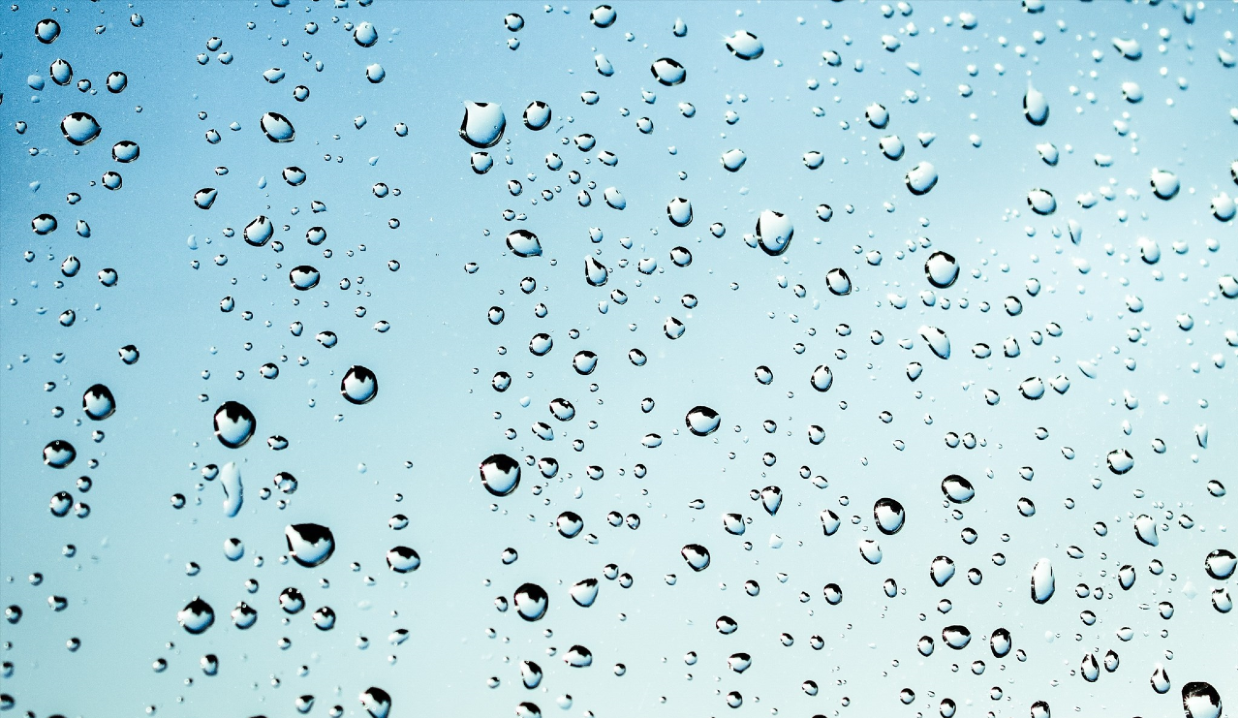
\includegraphics[width=\paperwidth]{Water3.png}};

\node[inner sep=0pt] (background) at (current page.north east) {
\includegraphics[scale=0.5, angle=-90]{BassettCTCLogo1.png}};
\node[inner sep=0pt] (background) at (8.1,-1) {
\includegraphics[scale=0.03, angle=0]{waterdrop.jpg}};

\draw (current page.center)node [fill=blue!1!white!10,fill opacity=.3,text opacity=1,inner sep=2cm]at (7,2){ \Huge\centering\bfseries\sffamily\parbox[c][][t]{\paperwidth}{\centering \textcolor{Bittersweet}{} \\\vspace{3cm}\textcolor{BurntOrange}{Drinking Water Treatment \& Distribution}\\[15pt] % Book title
% {\Large A Profound Subtitle}\\[20pt] % Subtitle
{}}}; % Author name
\end{tikzpicture}
%\begin{center}
%
\includegraphics[scale=1, angle=-90]{BassettCTCLogo1.png} 
%\end{center}












%\begin{tikzpicture}[]
%\path[help lines,step=.2] (0,0) grid (16,6);
%\path[help lines,line width=.6pt,step=1] (0,0) grid (16,6);
%
%\node[inner sep=0pt] (background) at (current page.center) {\includegraphics[width=\paperwidth]{WaterBackground1.png}};
%\draw (current page.center)node [fill=blue!1!white!10,fill opacity=.3,text opacity=1,inner sep=2cm] { \Huge\centering\bfseries\sffamily\parbox[c][][t]{\paperwidth}{\centering \textcolor{Bittersweet}{October 2022} \\\textcolor{BurntOrange}{Drinking Water Treatment}\\[15pt]
%
%  \pgftext{
\includegraphics[width=300pt, angle =-90]{BassettCTCLogo1.png}} at (16,5);
%%  \pgftext{\includegraphics[width=150pt]{pic2.png}} at (0,0);
%\end{tikzpicture}
\vfill
\endgroup

%----------------------------------------------------------------------------------------
%	COPYRIGHT PAGE
%----------------------------------------------------------------------------------------

\newpage
~\vfill
\thispagestyle{empty}

\noindent Copyright \copyright\ 2022 Shabbir Basrai\\ % Copyright notice
%
%\noindent \textsc{Published by Publisher}\\ % Publisher
%
%\noindent \textsc{book-website.com}\\ % URL
%
%\noindent Licensed under the Creative Commons Attribution-NonCommercial 3.0 Unported License (the ``License''). You may not use this file except in compliance with the License. You may obtain a copy of the License at \url{http://creativecommons.org/licenses/by-nc/3.0}. Unless required by applicable law or agreed to in writing, software distributed under the License is distributed on an \textsc{``as is'' basis, without warranties or conditions of any kind}, either express or implied. See the License for the specific language governing permissions and limitations under the License.\\ % License information, replace this with your own license (if any)

\noindent \textit{Revision Date: October 2022} % Printing/edition date

%----------------------------------------------------------------------------------------
%	TABLE OF CONTENTS
%----------------------------------------------------------------------------------------

%\usechapterimagefalse % If you don't want to include a chapter image, use this to toggle images off - it can be enabled later with \usechapterimagetrue

\chapterimage{WaterChapterImage} % Table of contents heading image

\pagestyle{empty} % Disable headers and footers for the following pages

\tableofcontents % Print the table of contents itself
\listoffigures
\listoftables
\cleardoublepage % Forces the first chapter to start on an odd page so it's on the right side of the book

\pagestyle{fancy} % Enable headers and footers again

%----------------------------------------------------------------------------------------
%	PART
%----------------------------------------------------------------------------------------



%----------------------------------------------------------------------------------------
%	CHAPTER 1
%----------------------------------------------------------------------------------------

% \chapterimage{chapter_head_2.pdf} % Chapter heading image

% \chapter{Text Chapter}

% \section{Paragraphs of Text}\index{Paragraphs of Text}



% \lipsum[1-7] % Dummy text
% 
%------------------------------------------------

%\section{Citation}\index{Citation}
%
%This statement requires citation \cite{article_key}; this one is more specific \cite[162]{book_key}.

%------------------------------------------------

%\section{Lists}\index{Lists}
%
%Lists are useful to present information in a concise and/or ordered way\footnote{Footnote example...}.
%
%\subsection{Numbered List}\index{Lists!Numbered List}
%
%\begin{enumerate}
%\item The first item
%\item The second item
%\item The third item
%\end{enumerate}
%
%\subsection{Bullet Points}\index{Lists!Bullet Points}
%
%\begin{itemize}
%\item The first item
%\item The second item
%\item The third item
%\end{itemize}
%
%\subsection{Descriptions and Definitions}\index{Lists!Descriptions and Definitions}
%
%\begin{description}
%\item[Name] Description
%\item[Word] Definition
%\item[Comment] Elaboration
%\end{description}


%----------------------------------------------------------------------------------------
%	PART 2
%----------------------------------------------------------------------------------------


%----------------------------------------------------------------------------------------
%	CHAPTER 1
%----------------------------------------------------------------------------------------

%\chapter{Wastewater Math}
%
\part{Module 1}
\chapterimage{CertificationCover}
\chapter{Water Systems Operator Certifications}\index{Operator license!Water systems operator certifications}
\section{Operator certification background}\index{Operator certification background}
\begin{itemize}
\item Federal law requires operators at water treatment plants for drinking water, wastewater, and recycled water, as well as those involved in the distribution of drinking water, to be State certified.  

\item For drinking water, California's State Water Resources Control Board's (SWRCB's) Drinking Water Operator Certification Program (DWOPCP) under its Drinking Water Operator Certification Program (DWOCP), is responsible for the testing and certification of water treatment and water distribution operators throughout the state of California.

\item For wastewater, the SWRCB's Wastewater Operator Certification program (WWOCP) administers Wastewater Treatment Plant Certification examinations, certifications (Grades I to V), and certification renewals.

\item The CA-NV AWWA currently offers voluntary Advanced Water Treatment Operator (AWTO) certifications for water and wastewater operators to meet the high demand for highly skilled and certified advanced water treatment operators.

\end{itemize}

\section{Operational activities}\index{Operator!Operational activities}
California laws stipulate that water systems shall utilize only certified operators to make decisions addressing the following operational activities:\\
\subsection{Drinking water treatment:}\index{Operator!Operational activities!Treatment}
Water treatment operators work in water treatment plants where water from wells, rivers, streams, and reservoirs is treated and distributed to customers. Water treatment plant operators typically do the following:
\begin{itemize}
\item Add chemicals, such as ammonia, chlorine, or lime, to disinfect water or other liquids.
\item Inspect equipment on a regular basis.
\item Monitor operating conditions, meters, and gauges.
\item Collect and test water and sewage samples.
\item Record meter and gauge readings, and operational data.
\item Operate equipment to purify and clarify water, or to process or dispose of sewage.
\item Clean and maintain equipment, tanks, filter beds, and other work areas.
\item Stay current on environmental laws and regulations.
\item Ensure safety standards are met.
\end{itemize}
\subsection{Water distribution:}\index{Operator!Operational activities!Distribution}
\begin{itemize}
\item Water distribution operators are responsible for the safe and efficient operation of water pumps, valves, and other equipment. They monitor gauges and meters to ensure that water is being distributed in a timely manner and at appropriate pressures.

\item Water distribution operators may also be tasked with maintaining or repairing any equipment that breaks down during their shift. This could include anything from replacing parts on pumps to fixing leaks in pipes or hoses.
\item Water distribution operators typically do the following:
\begin{itemize}
\item Install, tap, re-line, disinfect, test and connect water mains and appurtenances.
\item Shutdown, repair, disinfect and test broken water mains.
\item Oversee the flushing, cleaning, and pigging of existing water mains.
\item Pull, reset, rehabilitate, disinfect and test domestic water wells.
\item Stand-by emergency response duties for after hours distribution system operational emergencies.
\item Drain, clean, disinfect, and maintain distribution reservoirs.
\end{itemize}
\end{itemize}
Water systems shall utilize either certified distribution operators or treatment operators that have been trained to make decisions addressing the following operational activities:\\
\begin{itemize}
\item Operate pumps and related flow and pressure control and storage facilities manually or by using a system control and data acquisition (SCADA) system.
\item Maintain and/or adjust system flow and pressure requirements, control flows to meet consumer demands.
\item Determine and control proper chemical dosage rates for wellhead disinfection and distribution residual maintenance.
\item Investigate water quality problems in the distribution system.
\end{itemize}


\subsection{Wastewater treatment:}\index{Operator!Operational activities!Wastewater}
Wastewater operators typically do the following as part of their job responsibilities:
\begin{itemize}
\item Operate and maintain the wastewater treatment plant and collection systems.
\item Operate and adjust controls on treatment plant equipment and machinery, such as valves, pumps, and motors. 
\item Read and interpret meters and gauges.
\item Regulate plant effluent.
\item Monitor, repair, and maintain wastewater system lift stations; remove debris; disassemble and clean pumps; perform minor repairs when necessary. Locate problems and operate sewer cleaning equipment to clear blockages.
\item Performs routine maintenance and minor repairs on plant equipment, system equipment,
facilities, distribution system, and collection system.
\item Maintaining plant records and preparing monthly and quarterly reports.
\item Perform all aspects of sampling, monitoring, and testing required to maintain compliance with Federal, State, and Local regulations governing the wastewater treatment process, stormwater, and sludge management.
\end{itemize}

\subsection{Advanced treatment/water reuse:}\index{Operator!Operational activities!Advanced treatment/water reuse}
The Advanced Water Treatment Operators (AWTO) perform a full range of duties associated with operating and maintaining water treatment systems and equipment used for Advanced Water Treatment for water reuse.
AWTO typically do the following as part of their job responsibilities:\\
\begin{itemize}
\item Operate, monitor, and maintain AWT processes, such as membrane systems and advanced oxidation.
\item AWTOs have an advanced understanding of technologies and regulations pertinent to the end uses of treated water; such as recycled water, potable water, and potable water reuse.
\item At the supervisor and management level, maintain regular communication with regulatory agencies and ensure permit compliance. 
\item Responsibility for preparing and submitting regulatory reports.
\end{itemize}
\newpage
\section{Qualifications and eligibility}\index{Operator license!Qualifications and eligibility}
\subsection{Treatment}
\begin{table}[H]
\captionsetup{justification=centering}
\scriptsize

\begin{tabular}{|c|p{7.1cm}|p{7cm}|}
\hline
\thead{Grade} & \thead{Minimum Qualifications for Examination                                                                                                                                                                                                                                                                                     } & \thead{Eligibility Criteria for Certification                                                                                                                                                                                                                                                                                                                                                                                                                                                                                                } \\
\hline
T1    & High School Diploma / GED Equivalency*.                                                                                                                                                                                                                                                                                     & Successful completion of the Grade   T1 examination within the three years prior to   submitting certification application.                                                                                                                                                                                                                                                                                                                                                                                                            \\
\hline
T2    & \makecell[l]{High School Diploma / GED Equivalency*\\AND\\One 3-unit (or 36-hour) course of specialized training covering\\the fundamentals of drinking water treatment.} & \makecell[l]{Successful completion of the Grade T2 examination within\\the three years prior to submitting certification application.                                                                                                                                                                                                                                                                                                                                                                                                           } \\
\hline
T3    & \makecell[l]{High School Diploma / GED Equivalency*\\AND\\Two 3-unit (or 36-hour) courses of specialized training\\that include at least one course in drinking water treatment and a \\second course in either drinking water treatment, distribution,\\or wastewater treatment.}& \makecell[l]{Successful completion of the Grade T3 examination within the\\three years prior to   submitting certification application\\AND\\At least one year of operator experience working as a   certified\\T2 operator at a T2 facility or higher. This may be substituted\\with (3) below.\\AND\\      At least one additional year of operator experience working as a\\certified treatment operator. This may be substituted with\\(1), (2), or (4) below.}\\  
\hline                               
T4    & \makecell[l]{Current T3 certification\\AND\\Three 3-unit (or 36-hour) courses of specialized training that\\include at least two courses in the fundamentals of drinking\\water treatment and a third course in either\\drinking water treatment, distribution, or wastewater treatment.} & \makecell[l]{Successful completion of the Grade T4 examination within the\\three years prior to submitting the certification application\\AND\\At least one year of operator experience working as shift\\or chief operator, while a certified T3 operator at a T3\\facility or   higher. This may be substituted with (3) below.\\AND\\At least three additional years of operator experience\\working as a certified treatment operator. This may be\\substituted with (1) or (4) below.}\\
\hline
T5    & \makecell[l]{Current T4 certification\\AND\\Four 3-unit (or 36-hour) courses of specialized training that\\include\\at least two courses in drinking water treatment and two \\additional   courses in either drinking water treatment, \\distribution,or wastewater   treatment.}              & \makecell[l]{Successful completion of the Grade T5 examination within the\\three years prior to   submitting the application for certification\\AND\\At least two years of operator experience working as a   shift or\\chief operator, while a certified T4 operator at a T4 facility or \\ higher. There are no substitutions.\\AND\\At least three additional years of operator experience working\\ as a  certified treatment operator. This may be substituted with\\(1) or (4) below.} \\ 
\hline      
\end{tabular}
\caption{Water treatment license Exams - qualifications and eligibility}
\end{table}
\begin{tiny}
High School Diploma/GED equivalency for Grades 1 and 2 ONLY can be fulfilled with either successful completion of Basic Small Water Systems Operations course provided by the Department
OR 1 year as an operator of a facility that required an understanding of a chemical feeds, hydraulic systems, and pumps."\\			
Experience substitutions for certification, as referenced above.
\begin{enumerate}
\item A relevant degree earned at an accredited academic institution may be substituted as follows:
\begin{enumerate}[label=\alph*)]
\item Associate’s Degree or Certificate in Water or Wastewater Technology that includes at least 15 units of physical, chemical, or biological science may be used to fulfill 1 year of operator experience.
\item Bachelor’s Degree in engineering or in physical, chemical, or biological sciences (e.g Biology, Chemical Engineering, Chemistry, Civil Engineering, Environmental Engineering, Microbiology, Public Health, or Sanitary Engineering) may be used to fulfill 1.5 years of operator experience.
\item Master’s Degree in the above mentioned fields in (b) may be used to fulfill 2 years of operator experience.
\end{enumerate}
\item A certified operator may substitute, on a day-for-day basis, experience gained while working with lead responsibility for water quality related projects of research.
\item If an applicant has a Bachelor’s or Master’s of Science degree, completion of a comprehensive operator training program, may be substituted for the required experience.
\item Experience gained as a certified wastewater treatment operator may be used to substitute up to 2 years of the experience requirement. Wastewater treatment operator experience is credited on a two-for-one basis (i.e. 2 months in wastewater=1 month in drinking water).		
\end{enumerate}
\end{tiny}
\newpage
\subsection{Distribution}

\begin{table}[H]
\captionsetup{justification=centering}
\scriptsize

%\tiny, \scriptsize, \footnotesize, \small, \normalsize, \large, \Large, \LARGE, \huge, and \Huge.
\begin{tabular}{|c|p{7.1cm}|p{7cm}|}
\hline
\thead{Grade} & \thead{Minimum Qualifications for\\ Examination                                                                                                                                                                                                                                                                                            } & \thead{Eligibility Criteria for\\ Certification                                                                                                                                                                                                                                                                                                                                                                                                                      } \\ \hline


D1    & High School Diploma / GED Equivalency*                                                                                                                                                                                                                                                                                             & \makecell[l]{Successful completion of the Grade   D1 examination within \\the three years prior to\\submitting certification application.                                                                                                                                                                                                                                                                                                                                 } \\ 
\hline


D2    & \makecell[l]{High School Diploma / GED Equivalency*\\ AND\\ One 3-unit (or 36-hour) course of specialized training covering\\the fundamentals of water supply principles.} & \makecell[l]{Successful completion of the Grade D2 examination within \\the three years prior to submitting certification \\application}.                                                                                                                                                                                                                                                                                                                                \\ 
\hline


D3    & \makecell[l]{Current D2 Certification\\AND\\Two 3-unit (or 36-hour) courses of specialized training that\\includes at least one course in the fundamentals of water supply\\ principles and a second course in either drinking water\\distribution, treatment, or   wastewater treatment.} & \makecell[l]{Successful completion of the Grade D3 examination within\\the three years prior to submitting certification application\\AND\\At least one year of operator experience working as a certified\\D2 operator for a D2 system or higher\\AND\\At least one additional year of operator experience working\\as a distribution operator. This may be substituted with (1)\\or (2) below.}\\ 
\hline


D4    & \makecell[l]{Current D3 certification\\ AND \\Three 3-unit (or 36-hour) courses of specialized training\\that includes at least two courses in the fundamentals of water supply\\ principles and a third course in either drinking water distribution,\\treatment, or wastewater treatment.}& \makecell[l]{Successful completion of the Grade   D4 examination within the \\three years prior to submitting the application for certification\\ AND\\ At least one year of operator experience working as a\\certified D3 operator for a D3 system or higher\\ AND\\ At least three additional years of operator experience working\\as a distribution operator. This may be substituted with (1)\\or (2) below.}\\ \hline
D5    & \makecell[l]{Current D4 certification\\AND\\Four 3-unit (or 36-hour) courses of specialized training\\ that includes at least two courses in the fundamentals of water\\supply principles and two additional courses in either\\ drinking water distribution, treatment, or wastewater treatment.} & \makecell[l]{Successful completion of the Grade D5 examination within\\the three years prior to submitting the application for\\certification\\AND\\At least two years of operator experience working as a\\certified D4 operator for a D4 or D5 system\\AND\\At least three additional years of operator experience\\working as a distribution operator. This may be substituted\\with (1) or (2) below.}\\ \hline
\end{tabular}
\caption{Distribution license exams - qualifications and eligibility}
\end{table}

\begin{tiny}

High School Diploma/GED equivalency for Grades 1 and 2 ONLY can be fulfilled with either successful completion of Basic Small Water Systems Operations course provided by the Department OR 1 year as an operator of a facility that required an understanding of a piping system that included pumps, valves, and storage tanks.\\

Experience substitutions for certification, as referenced above.
\begin{enumerate}[]
\item A relevant degree earned at an accredited academic institution may be substituted as follows:
\begin{enumerate}[label=(\alph*)]
\item Associate’s Degree or Certificate in Water or Wastewater Technology that includes at least 15 units of physical, chemical, or biological science may be used to fulfill 1 year of operator experience.
\item Bachelor’s Degree in engineering or in physical, chemical, or biological sciences (e.g. Biology, Chemical Engineering, Chemistry, Civil Engineering, Environmental Engineering, Microbiology, Public Health, or Sanitary Engineering) may be used to fulfill 1.5 years of operator experience.
\item Master’s Degree in the above mentioned fields in (b) may be used to fulfill 2 years of operator experience.
\end{enumerate}
\item A certified operator may substitute, on a day-for-day basis, 1 additional year of operator experience working as a distribution operator with experience gained while working with lead responsibility for water quality or quantity related projects or research.
\end{enumerate}	
\end{tiny}

\newpage
\subsection{Wastewater}
\begin{table}[H]
\captionsetup{justification=centering}
\scriptsize
\begin{tabular}{|l|p{6.5cm}|l|p{6.5cm}|}
\hline

\multicolumn{1}{|c|}{\thead{PATH}} & 
  \multicolumn{1}{|c|}{\thead{EXAMINATION EDUCATION REQUIREMENTS}} & &\multicolumn{1}{|c|}{\thead{CERTIFICATION QUALIFYING EXPERIENCE \\REQUIREMENTS}}\\\hline


%\thead{PATH} & \thead{EXAMINATION EDUCATION REQUIREMENTS}&     &\thead{CERTIFICATION QUALIFYING EXPERIENCE \\REQUIREMENTS}\\ \hline
GRADE I   &                                                                                                                                                                                                                                                                                               &     &                                                                                                 \\ \hline
1         & High  school  diploma or equivalent and 6 educational pts                                                                                                                                                                                                                          & and & 1 year of full-time qualifying experience                                   \\ \hline
GRADE II  &                                                                                                                                                                                                                                                                                               &     &                                                                                                 \\ \hline
1         & High  school  diploma    or  equivalent  and    9 educational pts                                                                                                                                                                                                                          & and & 18   months   of     full-time   qualifying   experience as a Grade I operator                  \\ \hline
2         & High  school  diploma    or  equivalent  and    12 educational pts                                                                                                                                                                                                                         & and & 2    years    of      full-time    qualifying   experience                                      \\ \hline
3         & \makecell[l]{Associate’s  degree,  a    higher  degree,  or  a minimum   of\\   60  college   semester   units, including a minimum of 15\\semester units of science courses                                                                                                                          } & and & 1     year     of       full-time     qualifying   experience                                   \\ \hline
GRADE III &                                                                                                                                                                                                                                                                                               &     &                                                                                                 \\ \hline
1         & High  school  diploma    or  equivalent  and    12 educational pts                                                                                                                                                                                                                         & and & 3    years    of      full-time    qualifying   experience as a Grade II operator               \\ \hline
2         & High  school  diploma    or  equivalent  and    18 educational pts                                                                                                                                                                                                                         & and & 4    years    of      full-time    qualifying   experience                                      \\ \hline
3         & \makecell[l]{Associate’s  degree  or    a  minimum   of     60 college semester\\ units,including a minimum of 15 semester units of\\science courses                                                                                                                                                      } & and & 2    years    of      full-time    qualifying   experience                                      \\ \hline
4         & \makecell[l]{Bachelor’s   degree   or     a   higher   degree, including a\\ minimum of 30 semester   units of science courses                                                                                                                                                                              } & and & 1     year     of       full-time     qualifying   experience                                   \\ \hline
GRADE IV  &                                                                                                                                                                                                                                                                                               &     &                                                                                                 \\ \hline
1         & High  school  diploma    or  equivalent  and    32 educational points                                                                                                                                                                                                                         & and & 6    years    of      full-time    qualifying   experience                                      \\ \hline
2         & \makecell[l]{Associate’s   degree   or     a  minimum   of     60 college semester \\units, including a minimum of 15 semester units of   science\\ courses                                                                                                                                                   } & and & 4    years    of      full-time    qualifying   experience                                      \\ \hline
3         & \makecell[l]{Bachelor’s   degree   or     a   higher   degree, including a minimum\\ of 30 semester   units of science courses                                                                                                                                                                              } & and & 3    years    of      full-time    qualifying   experience                                      \\ \hline
4         &\makecell[l]{ Valid  registration  as    a  chemical,  civil,\\or mechanical     engineer     issued     by the California  Board \\ for    Professional  Engineers and  Land    Surveyors  or  by\\ another  state, territory, or   Indian tribe                                                   } & and & 2    years    of      full-time    qualifying   experience                                      \\ \hline
GRADE V   &                                                                                                                                                                                                                                                                                               &     &                                                                                                 \\ \hline
1         & High  school  diploma    or  equivalent  and    48 educational points                                                                                                                                                                                                                         & and & 10      years      full-time      qualifying experience                                         \\ \hline
2         & \makecell[l]{Associate’s   degree   or     a  minimum   of     60 college semester \\units, including a minimum of 15 semester units of   science\\courses                                                                                                                                                   } & and & 6    years    of      full-time    qualifying   experience                                      \\ \hline
3         & Bachelor’s   degree   or     a   higher   degree, including a minimum of 30 semester   units of science courses                                                                                                                                                                               & and & 5    years    of      full-time    qualifying   experience                                      \\ \hline
4         & \makecell[l]{Valid  registration  as    a  chemical,  civil,    or mechanical\\ engineer issued by the California  Board  for    Professional\\  Engineers and Land    Surveyors or  by another  state,  a \\territory, or an Indian tribe} & and & 4    years    of      full-time    qualifying   experience                                      \\ \hline
\end{tabular}
\caption{Wastewater operator license exams requirements}
\end{table}

\begin{itemize}
\scriptsize
\item 1,800 hours of qualifying experience as an Operator-In-Training (OIT) \index{Operator-in-training (OIT)} at a wastewater treatment plant (WWTP) is required to become a certified operator. The 1,800 OIT hours counts as one year of full-time qualifying experience.
\item OIT applicants must submit a copy of a high school diploma or equivalent and six educational points.
\item Volunteer, part-time, full-time and overtime hours qualify.
\item OIT hours are not grade level specific and OIT experience does NOT expire.
\item OIT certificates are good for three years from the date of issuance and can be renewed.  To renew an OIT certificate, an applicant must have taken and passed a Wastewater Exam within the last four years.
\end{itemize}
\newpage
\subsection{Advanced water treatment or water reuse}
\begin{table}[H]
\captionsetup{justification=centering}
\scriptsize
\begin{tabularx}{\textwidth}{| X | X |}
%{
%|>{\setlength\hsize{1.\hsize}\setlength\linewidth{\hsize}}X|
%>{\setlength\hsize{.5\hsize}\setlength\linewidth{\hsize}}X|
%>{\setlength\hsize{.01\hsize}\setlength\linewidth{\hsize}}X|}

\hline
\multicolumn{2}{|l|}{Grade 3}                                                                                                                                                                                                                                                                                                                                                                                                   \\
\hline
\begin{itemize}
\item Possess a current state issued Drinking Water Treatment Operator Certification or Wastewater Treatment Plant   Operator Certification, Grade III or higher                                                                                                                                                                                             
\end{itemize} & 
\begin{itemize}
\item Successful completion of AWTO Grade 3 Exam (AWT3TM)
\end{itemize} \\
\hline
\multicolumn{2}{|l|}{Grade 4}                                                                                                                                                                                                                                                                                                                                                                                                   \\
\hline
\begin{itemize}
\item Possess a current AWT3 certification
\item 2 years of   experience with one or more AWT processes (see Table 1). Retroactive   experience prior to AWT3 certification may be included 
\end{itemize}
& 
\begin{itemize}
\item Successful   completion of AWTO Grade 4 Exam (AWT4TM) 
\end{itemize}\\
\hline
\multicolumn{2}{|l|}{Grade 5}                                                                                                                                                                                                                                                                                                                                                                                                  \\
\hline
\begin{itemize} 
\item Possess a   current AWT4 certification 
\item 3 years of   experience to include 2 years of experience in at least one AWT process and 1   additional year with at least 2 AWT processes in a single treatment train   (see Table 1). Retroactive experience prior to AWT4 certification may be   included. 
\end{itemize}
&\begin{itemize}
\item Successful completion of AWTO Grade 5 Exam (AWT5TM)
\end{itemize}\\
\hline
\end{tabularx}

\caption{Advanced water treatment certification requirements}
\end{table}
\begin{table}[H]
\captionsetup{justification=centering}
\scriptsize
\begin{center}
\begin{tabular}{|l|p{2cm}|p{2cm}|p{2cm}|}
\hline
 & \begin{center}  {Exam Fee} \end{center} & \begin{center}{Reexamination Fee}  \end{center} & \begin{center}{Application Fee}  \end{center}\\
\hline
D1 \& T1 & \multicolumn{1}{|c|}{\$50} & \multicolumn{1}{|c|}{ \$30} & \multicolumn{1}{|c|}{\$70}\\
\hline
D2 \& T2  & \multicolumn{1}{|c|}{\$65} & \multicolumn{1}{|c|}{\$45} & \multicolumn{1}{|c|}{\$80}\\
\hline
D3 \& T3 & \multicolumn{1}{|c|}{\$100} & \multicolumn{1}{|c|}{\$70} & \multicolumn{1}{|c|}{\$120}\\
\hline
D4 \& T4 & \multicolumn{1}{|c|}{\$130}& \multicolumn{1}{|c|}{\$95}& \multicolumn{1}{|c|}{\$140}\\
\hline
D5 \& T5 & \multicolumn{1}{|c|}{\$155}& \multicolumn{1}{|c|}{\$120}& \multicolumn{1}{|c|}{\$140}\\
\hline
WW Grade I & \multicolumn{1}{|c|}{\$50} & \multicolumn{1}{|c|}{ \$30} & \multicolumn{1}{|c|}{\$95}\\
\hline
WW Grade II  & \multicolumn{1}{|c|}{\$65} & \multicolumn{1}{|c|}{\$45} & \multicolumn{1}{|c|}{\$125}\\
\hline
WW Grade III  & \multicolumn{1}{|c|}{\$100} & \multicolumn{1}{|c|}{\$70} & \multicolumn{1}{|c|}{\$170}\\
\hline
WW Grade IV & \multicolumn{1}{|c|}{\$130}& \multicolumn{1}{|c|}{\$95}& \multicolumn{1}{|c|}{\$190}\\
\hline
WW Grade V  & \multicolumn{1}{|c|}{\$155}& \multicolumn{1}{|c|}{\$120}& \multicolumn{1}{|c|}{\$190}\\
\hline
\multirow{2}{*}{AWWA - AWTO Grades III - V} & \multicolumn{3}{|l|}{\$250 - for Members of CA-NV AWWA, CWEA or both} \\
&\multicolumn{3}{|l|}{\$350 - for Non-Members of either association}\\
\hline
\end{tabular}
\caption{Exam and application fees}
\end{center}
\end{table}
\section{Expected range of knowledge}
\subsection{Treatment}
The Expected Range of Knowledge for Drinking Water Treatment Exam is provided in Appendix \ref{appendix:Treatment Exam - ROK}.\\
\subsection{Distribution}
The Expected Range of Knowledge for Drinking Water Distribution Exam is provided in Appendix \ref{appendix:Distribution Exam - ROK}.\\
\subsection{Wastewater}
Details for each of the Grades I-V Wastewater Operator License Exams is provided in Appendix \ref{appendix:Wastewater Exams}.\\
\section{Certification requirements}\index{Water Operator!certification requirements}
\subsection{Treatment}
\begin{itemize} 
\item Treatment systems are classified as T1-T5, according to a point system that takes into account various source water characteristics, maximum capacity and treatment techniques. Appendix \ref{appendix:Water Treatment Facilities Classification} provides details on the classification of water treatment facilities.\\
\begin{table}[H]
\begin{center}
\captionsetup{justification=centering}
\begin{tabular}{|l|c|}
\hline
Total Points & Class\\
\hline
Less than 20 & T1\\
\hline
20 through 39 & T2\\
\hline
40 through 59&  T3\\
\hline
60 through 79 & T4\\
\hline
80 or more & T5\\
\hline
\end{tabular}
\caption{Water treatment facility class designations}
\end{center}
\end{table}

\item Any person operating a water treatment plant is required to possess a valid, unexpired water treatment operator certificate of appropriate grade.

\item The certification requirements of the Chief Treatment Plant Operator and that of the Shift Operator - persons  in responsible charge of the water treatment plant,  are required to possess a valid, unexpired water treatment operator certificate equal to or greater than the classification of the water treatment plant.

\begin{table}[H]
\begin{center}
\begin{tabular}{|c|c|c|}
\hline
\begin{tabular}{c}
Total Points \\
Class \\
\end{tabular} & \begin{tabular}{c}
Minimum Certification of \\
Chief Operator \\
\end{tabular} & \begin{tabular}{c}
Minimum Certification \\
of Shift Operator \\
\end{tabular} \\
\hline
T1 & T1 & T1 \\
\hline
T2 & T2 & T1 \\
\hline
T3 & T3 & T2 \\
\hline
T4 & T4 & T3 \\
\hline
T5 & T5 & T3 \\
\hline
\end{tabular}
\caption{Minimum certification requirements for Chief and Shift Operators}\index{Minimum certification requirements for treatment plants' chief and shift operators}
\end{center}
\end{table}
\end{itemize}
\newpage
\subsection{Distribution}
\begin{itemize}
\item Distribution systems are classified as D1 to D5 by population served and system complexity. The population categories are:\\
\begin{table}[H]
\begin{center}
\captionsetup{justification=centering}
\begin{tabular}{|l|c|}
\hline
\textbf{Class} & \textbf{Population Served} \\
\hline
D1 & $\leq$1,000\\
\hline
D2 & 1,001 - 10,000\\
\hline
D3 &  10,001 - 50,000\\
\hline
D4 & 50,001 - 5 million\\
\hline
D5 & $\geq$5 million\\
\hline
\end{tabular}
\caption{Distribution systems class designations}
\end{center}
\end{table} 
\item Distribution systems can be upgraded one level due to complexity, using a point system which takes into account: number of pressure zones, storage reservoirs and uncovered storage reservoirs, treatment, the size of the largest pump utilized, and customers with a nonpotable water supply connection. 
\item A person who operates a water distribution system shall possess a valid, unexpired water distribution operator certificate of the appropriate grade in accordance with the regulations.
\item  A person who is in responsible charge of the water distribution system shall possess a valid, unexpired water distribution operator certificate equal to or greater than the classification of the water distribution system.
\end{itemize}
\begin{table}[H]
\begin{center}
\begin{tabular}{|c|c|c|}
\hline
\begin{tabular}{c}
\textbf{Distribution System} \\
\textbf{Classification} \\
\end{tabular} & \begin{tabular}{c}
\textbf{Minimum Certification of} \\
\textbf{Chief Operator} \\
\end{tabular} & \begin{tabular}{c}
\textbf{Minimum Certification} \\
\textbf{of Shift Operator} \\
\end{tabular} \\
\hline
D1 & D1 & D1 \\
\hline
D2 & D2 & D1 \\
\hline
D3 & D3 & D2 \\
\hline
D4 & D4 & D3 \\
\hline
D5 & D5 & D3 \\
\hline
\end{tabular}
\caption{Minimum certification requirements for Chief and Shift Operators}\index{Minimum certification requirements for distribution systems' chief and shift operators}
\end{center}
\end{table}
\newpage
\subsection{Wastewater}
\begin{itemize}
\item All wastewater plant operators are required to possess at least a valid Grade I certificate, a valid provisional operator certificate, or a valid operator-in-training certificate.
\item Wastewater treatment plants are classified as Class I to V based upon the plant design flow and treatment process. 
\begin{table}[H]
\begin{center}
\begin{tabular}{|c|l|l|}
\hline
{\textbf{Class} }                    & \multicolumn{1}{c|}{ \textbf{Treatment Process}} & \multicolumn{1}{c|}{\textbf{Design Flow (MGD)}} \\ \hline
\multirow{2}{*}{I}                       & Pond                                                  & All                                                   \\ \cline{2-3} 
                                         & Primary                                               & 1 or less                                           \\ \hline
\multirow{3}{*}{II}                      & Primary                                               & Greater than 1 through 5                          \\ \cline{2-3} 
                                         & Biofiltration                                         & 1 or less                                           \\ \cline{2-3} 
                                         & Extended Aeration                                     & All                                                   \\ \hline
\multirow{4}{*}{III}                     & Primary                                               & Greater than 5 through 20                         \\ \cline{2-3} 
                                         & Biofiltration                                         & Greater than 1 through 10                         \\ \cline{2-3} 
                                         & Activated Sludge                                      & 5 or less                                           \\ \cline{2-3} 
                                         & Tertiary                                              & 1 or less                                           \\ \hline
\multirow{4}{*}{IV}                      & Primary                                               & Greater than 20                                     \\ \cline{2-3} 
                                         & Biofiltration                                         & Greater than 10 through 30                        \\ \cline{2-3} 
                                         & Activated Sludge                                      & Greater than 5 through 20                         \\ \cline{2-3} 
                                         & Tertiary                                              & Greater than 1 through 10                         \\ \hline
\multicolumn{1}{|l|}{\multirow{3}{*}{V}} & Biofiltration                                         & Greater than 30                                     \\ \cline{2-3} 
\multicolumn{1}{|l|}{}                   & Activated Sludge                                      & Greater than 20                                     \\ \cline{2-3} 
\multicolumn{1}{|l|}{}                   & Tertiary                                              & Greater than 10                                     \\ \hline
\end{tabular}
\caption{Wastewater treatment plant classification}\label{Wastewater treatment plant classification}\index{Wastewater treatment plant classification}
\end{center}
\end{table}
\item For each plant class, WWOCP sipulates that the Chief plant operator and designated operator-in- charge shall possess a valid operator certificate at a grade level at least equivalent as provided to the following: 
\end{itemize}
\begin{table}[H]
\begin{center}
\begin{tabular}{|c|c|c|}
\hline
\begin{tabular}{c}
Wastewater \\
Treatment Plant \\
Classification \\
\end{tabular} & \begin{tabular}{c}
Minimum Grade Level of \\
Chief Plant Operator \\
\end{tabular} & \begin{tabular}{c}
Minimum Grade Level of \\
Designated Operator-in-Charge \\
\end{tabular} \\
\hline
I & I & I \\
\hline
II & II & I \\
\hline
III & III & II \\
\hline
IV & IV & III \\
\hline
\end{tabular}
\end{center}
\end{table}
\newpage
\subsection{Advanced water treatment}
\begin{itemize}
\item Per California laws, a water treatment plant operator may operate a water recycling treatment plant at a grade level appropriate for the class of wastewater treatment plant being operated.
 \begin{table}[H]
\begin{center}
\begin{tabular}{|c|c|c|}
\hline
\begin{tabular}{c}
Wastewater Treatment \\
Plant Classification \\
\end{tabular} & \begin{tabular}{c}
Water Treatment Plant \\
Operator Certificate \\
\end{tabular} & \begin{tabular}{c}
Wastewater Treatment Plant \\
Operator Certificate \\
\end{tabular} \\
\hline
I & T1 & Grade I \\
\hline
II & T2 & Grade II \\
\hline
III & T3 & Grade III \\
\hline
IV & T4 & Grade IV \\
\hline
V & T5 & Grade V \\
\hline
\end{tabular}
\caption{Certificate requirements for water recycling treatment plants}
\end{center}
\end{table}
\end{itemize}
\section{Certification renewal}\index{Water Operator!Certification renewal}
\begin{itemize}
\item Certification must be renewed every 3 years, or at least 120 days, but not more than 180 days, before the expiration date. 
\item Operators are expected to complete required number of continuing education contact hours during their renewal period. The continuing education requirements to renew a California water operator certificate are as follows:  \\
\item Continuing education are courses, classes or seminars that present “information related to the operation of a drinking water treatment facility and/or distribution system.”  Continuing education hours can be earned by attending water industry 
meetings, conferences, workshops, in-­house training, college courses, correspondence 
courses and internet classes.
\item There are no continuing education requirements for wastewater operator certification renewal. 
\end{itemize}
\begin{table}[H]
\begin{center}
\begin{tabular}{|p{2cm}|p{8cm}|}
\hline

\begin{center}{\textbf{Exam}}\end{center} & \begin{center}{\textbf{Required Continuing Education Contact Hours}}\end{center}\\
\hline
D1, T1 & 12 hours\\
\hline
D2, T2 & 16 hours\\
\hline
D3, T3 & 24 hours\\
\hline
D4, T4 & 36 hours\\
\hline
D5, T5 & 36 hours\\
\hline
\multicolumn{2}{|l|}{Up to 25\% of contact hours can be fulfilled by completing safety training.}\\
\hline
\end{tabular}
\caption{Certificate renewal contact hours requirements}
\end{center}
\end{table}
\newpage
\begin{table}[ht!]
\captionsetup{justification=centering}
\scriptsize
\begin{center}
\begin{tabular}{|c|p{2cm}|p{2cm}|}
\hline
 & \begin{center}{Triennial renewal}\end{center} & \begin{center}{Discounted certification and renewal}\end{center}\\
\hline
D1 \& T1 & \multicolumn{1}{|c|}{\$70} & \multicolumn{1}{|c|}{\$55$^1$}\\
\hline
D2 \& T2  & \multicolumn{1}{|c|}{\$80} & \multicolumn{1}{|c|}{\$60$^1$}\\
\hline
D3 \& T3 & \multicolumn{1}{|c|}{\$120} & \multicolumn{1}{|c|}{\$90$^1$}\\
\hline
D4 \& T4 & \multicolumn{1}{|c|}{\$140}& \multicolumn{1}{|c|}{\$105$^1$}\\
\hline
D5 \& T5 &  \multicolumn{1}{|c|}{\$140}& \multicolumn{1}{|c|}{\$105$^1$}\\
\hline
WW Grades I - V & \multicolumn{1}{|c|}{\$150}& \multicolumn{1}{|c|}{\$115$^2$}\\
\hline
\multicolumn{3}{|l|}{$^1$ For operators with both a water treatment and water }\\ \multicolumn{3}{|l|}{ \hspace{0.27cm}distribution certificates}\\
\multicolumn{3}{|l|}{$^2$ For operators with both a wastewater and water}\\ \multicolumn{3}{|l|}{   \hspace{0.27cm}treatment/distribution certificate}\\
\hline

\end{tabular}
\caption{Certificate renewal fees}
\end{center}
\end{table}






\part{Module 2}
\chapterimage{ChapterImageLaboratory.png} % Chapter heading image

\chapter{Water Quality \& Laboratory Procedures}





% Please add the following required packages to your document preamble:
% \usepackage[normalem]{ulem}
% \useunder{\uline}{\ul}{}
% Please add the following required packages to your document preamble:
% \usepackage[normalem]{ulem}
% \useunder{\uline}{\ul}{}
\begin{table}[H]
\begin{tabular}{| m{1cm} | m{15cm} |}
\hline
\multicolumn{2}{|l|}{\textbf{Expected   Range of Knowledge for Water Properties and Sources}}                                                                          \\ \hline
\multicolumn{2}{|l|}{\textit{Water   Distribution System Operator License Exams}}                                                                                      \\ \hline

D1 & Ability to read   a graduated cylinder                                                            \\ \hline
D1 & Ability to interpret   coliform test results                                                      \\ \hline
D1 & Knowledge of coliform   analysis methods                                                          \\ \hline
D1 & Knowledge of coliform   bacteria types                                                            \\ \hline
D1 & Knowledge of the   definition of pathogenic organisms                                             \\ \hline
D1 & Knowledge of holding   times (e.g. preservatives)                                                 \\ \hline
D1 & Knowledge of water   sampling techniques for bacteriological, organic, and inorganic constituents \\ \hline
D2 & Knowledge of the use   of coliform as a surrogate                                                 \\ \hline
D2 & Ability to   distinguish between presumptive and confirmed results                                \\ \hline
D2 & Knowledge of nitrate   formation in a distribution system                                         \\ \hline
D2 & Knowledge of   potential waterborne diseases                                                      \\ \hline
D2 & Knowledge of the   effects of abnormal pH levels in a distribution system                         \\ \hline
D2 & Knowledge of the   effects of hardness in a distribution system                                   \\ \hline
D2 & Knowledge of the   effects of heterotrophic bacteria in a distribution system                     \\ \hline
D3 & Knowledge of the   galvanic series                                                                \\ \hline
D3 & Knowledge of the   Langelier Index                                                                \\ \hline
D3 & Knowledge of common   inorganic contaminant compounds pH, Conductivity, Hardness, and Turbidity   \\ \hline
D3 & Knowledge of common   organic contaminant compounds                                               \\ \hline
D3 & Knowledge of sources   of inorganic contaminants in a distribution system                         \\ \hline
D3 & Knowledge of sources   of organic contaminants in a distribution system                           \\ \hline
D4 & Ability to interpret a Langelier Index                                                            \\ \hline

\end{tabular}
\end{table}


\newpage



\begin{table}[H]
\begin{tabular}{| m{1cm} |m{15cm} |}
\hline
\multicolumn{2}{|l|}{\textbf{Expected   Range of Knowledge for Water Properties and Sources}}                                                                      \\ \hline
\multicolumn{2}{|l|}{\textit{Water   Treatment Operator License Exams}}                                                                  \\ \hline
T1 & Ability to recognize   abnormal chemical characteristics of water                                 \\ \hline
T1 & Ability to recognize   abnormal odors or colors                                                   \\ \hline
T1 & Knowledge of   chemicals that contribute alkalinity and hardness to water                         \\ \hline
T1 & Knowledge of common   chemical and microbial contaminants in raw water                            \\ \hline
T1 & Knowledge of problems   caused by hard water                                                      \\ \hline
T1 & Knowledge of the   chemical components of groundwater and surface water                           \\ \hline
T1 & Ability to interpret   turbidity information                                                      \\ \hline
T1 & Knowledge of   turbidity causing matter                                                           \\ \hline
T1 & Knowledge of   chemicals that contribute hardness to water                                        \\ \hline
T1 & Ability to recognize   corrosion problems                                                         \\ \hline
T1 & Knowledge of pH   adjustment procedures                                                           \\ \hline
T1 & Knowledge of   corrosion causes                                                                   \\ \hline
T1 & Knowledge of abnormal   taste and odors                                                           \\ \hline
T1 & Knowledge of   chemicals that contribute taste and odor                                           \\ \hline
T1 & Knowledge of taste   and odor treatment processes                                                 \\ \hline
T1 & Ability to recognize   an iron and manganese problem                                              \\ \hline
T1 & Knowledge of health   effects of lead and copper                                                  \\ \hline
T1 & Knowledge of adverse   health effects caused by common contaminants                               \\ \hline
T1 & Ability to collect a   water sample                                                               \\ \hline
T1 & Ability to determine   a proper sampling site                                                     \\ \hline
T1 & Ability to follow   chain of custody                                                              \\ \hline
T1 & Knowledge of   appropriate sample containers and sample sizes                                     \\ \hline
T1 & Knowledge of maximum   holding times                                                              \\ \hline
T1 & Knowledge of proper   sampling and preservation techniques                                        \\ \hline
T1 & Knowledge of well   sampling techniques                                                           \\ \hline
T1 & Knowledge of chemical   hazards                                                                   \\ \hline
T1 & Ability to analyze a   water sample for free and total chlorine                                   \\ \hline
T1 & Ability to read and   interpret a colorimeter                                                     \\ \hline
T1 & Knowledge of approved   analytical procedures for chlorine analysis                               \\ \hline
T1 & Ability to read and   interpret a pH meter                                                        \\ \hline
T1 & Knowledge of acids   and bases                                                                    \\ \hline
T1 & Knowledge of   acceptable water pH range                                                          \\ \hline
T1 & Knowledge of   chemicals that affect the pH of water                                              \\ \hline
T1 & Knowledge of the   effects of pH on water quality                                                 \\ \hline
T1 & Knowledge of the pH   scale                                                                       \\ \hline
T1 & Ability to analyze a   water sample for pH                                                        \\ \hline
T1 & Ability to analyze a   water sample for turbidity                                                 \\ \hline
T1 & Ability to read and   interpret a turbidimeter                                                    \\ \hline
T1 & Knowledge of the   Nephelometric Turbidity Unit (NTU) scale                                       \\ \hline
T1 & Knowledge of   turbidimeter instrumentation                                                       \\ \hline
T1 & Knowledge of   turbidity level requirements                                                       \\ \hline
T1 & Ability to identify   an objectionable taste or odor in water                                     \\ \hline
T1 & Knowledge of   chemicals that contribute taste and odor to water                                  \\ \hline
T1 & Knowledge of the   presence/absence test method                                                   \\ \hline
T1 & Knowledge of approved   analytical procedures for coliform analysis                               \\ \hline
T1 & Knowledge of common   microbial contaminants in raw water                                         \\ \hline
T1 & Ability to interpret   water quality characteristics (hardness, turbidity, pH )                   \\ \hline
\end{tabular}
\end{table}
\newpage



\begin{table}[H]
\begin{tabular}{| m{1cm} |m{15cm} |}
\hline
\multicolumn{2}{|l|}{\textbf{Expected   Range of Knowledge for Water Properties and Sources}}                                                                      \\ \hline
\multicolumn{2}{|l|}{\textit{Water   Treatment System Operator License Exams (Continued)}}                                                                  \\ \hline
T1 & Ability to recognize   abnormal chemical characteristics of water                                 \\ \hline
T2 & Ability to prepare   and calibrate turbidimeter with Primary Standard (Formazin)                  \\ \hline
T2 & Ability to analyze a   water sample for water hardness                                            \\ \hline
T2 & Ability to recognize   abnormal colors in water                                                   \\ \hline
T2 & Knowledge of   Heterotrophic Plate Count (HPC)                                                    \\ \hline
T3 & Knowledge of the   Langelier Index                                                                \\ \hline
T3 & Knowledge of   corrosion control chemical reactions                                               \\ \hline
T3 & Knowledge of iron and   manganese oxidation chemistry                                             \\ \hline
T3 & Knowledge of   chemicals that contribute alkalinity to water                                      \\ \hline
T3 & Ability to use a   titrator                                                                       \\ \hline
T3 & Ability to recognize   a titration endpoint                                                       \\ \hline
T3 & Knowledge of abnormal   alkalinity levels                                                         \\ \hline
T3 & Ability to analyze a   water sample for specific conductance                                      \\ \hline
T3 & Ability to read and   interpret a specific conductance meter                                      \\ \hline
T3 & Knowledge of abnormal   color levels                                                              \\ \hline
T3 & Ability to   distinguish between presumptive and confirmed coliform results                       \\ \hline
T3 & Knowledge of the   multiple tube fermentation method                                              \\ \hline
T3 & Knowledge of the   membrane filtration method                                                     \\ \hline
T4 & Knowledge of the   health effects of fluoride                                                     \\ \hline
T4 & Ability to calculate   a TDS value from a specific conductance reading                            \\ \hline
T4 & Knowledge of EC/TDS   ratio                                                                       \\ \hline
T4 & Ability to calibrate   a specific conductance meter                                               \\ \hline
T4 & Ability to operate an   Ion Specific Electrode (ISE)                                              \\ \hline
T4 & Knowledge of optimal   fluoride level range                                                       \\ \hline
T4 & Knowledge of color   analysis scale                                                               \\ \hline
T4 & Knowledge of true and   apparent color                                                            \\ \hline
T4 & Knowledge of odor   analysis protocol                                                             \\ \hline
\end{tabular}
\end{table}

\newpage
Water occurring in nature will have other elements dissolved or suspended in it. A "contaminant" is a physical, chemical, biological, or radiological substance or matter, in water.  The type and amount of these contaminants will affect the property and safety of that water, if it is to be used as drinking water.  Some drinking water contaminants may be harmful if consumed at certain levels in drinking water while others may be harmless. The presence of contaminants does not necessarily indicate that the water poses a health risk.\\

Contaminants in drinking water can be broadly categorized as:
\begin{itemize}
\item \ul{Chemical contaminants} \index{Chemical contaminants} which may be naturally occurring or man-made elements or compounds. Examples of chemical contaminants include nitrogen, bleach, salts, pesticides, metals, and human or animal drugs.
\item \ul{Biological contaminants} \index{Biological contaminants} which are also refered as micorbes or microbiological contaminants which include bacteria, viruses, protozoa and parasites.
organisms
\item \ul{Radiological contaminants} \index{Radiological contaminants} which are chemical compounds or elements which contain unstable atoms that emit ionizing radiation.  Example of radiological contaminants include, cesium, plutonium and uranium.
\end{itemize}

\section{Organics}\index{Organics}
\begin{itemize}
\item Organics – are carbon based material can originate from lifeforms or can be man-made.
\item Only few carbon compounds such as carbonates, cyanides are not classified as organic.
\item In water they originate from decaying plant and animal life and wastes.
\item Amount present in natural waters is usually low. 
\item Many organic compounds are soluble in water, and surface waters are more prone to contamination by natural organic compounds than are groundwaters.
\item Synthetic organic compounds, such as polychlorinated biphenyls (PCBs), dioxin, and dichlorodiphenyl-trichloroethane (DDT), all of which are toxic, often persist and accumulate because they do not readily break down in natural ecosystems. 
\item Many of the organic compounds found in water are known to cause cancer and birth defects in people. 
\item Organic matter in water is responsible for:
\begin{itemize}
\item Color formation
\item Taste and odor problems
\item Oxygen depletion in streams
\item Interference with water treatment processes, and
\item Formation of halogenated compounds when chlorine is added to disinfect water.
\end{itemize}
\item The quantity of oxygen-consuming organics in water is usually determined by measuring its biochemical oxygen demand (BOD)\index{Organics!Quantification!Biochemical oxygen demand (BOD)}
\item BOD is the amount of dissolved oxygen required by aerobic decomposers to break down the organic materials in a given volume of water over a 5-day incubation period at 20\degree{C} (68\degree{F}).
\end{itemize}

\section{Inorganics} \index{Inorganics}
Inorganic elements do not contain carbon and are not derived from living material. The inorganics include metals, acids, bases, salts, oxides, sulfate, phosphates, etc.
\subsection{Metals}\index{Metals}
\begin{itemize}
\item Iron and Manganese:\\
\begin{itemize}
\item Although iron and manganese are most commonly found metals in groundwaters, surfacewaters may also contain significant amounts at times. 
\item Non-pathogenic bacteria feed on iron and manganese in water to form red-brown (iron) or black-brown (manganese) slime which accumulates on spouts and inside toilet tanks.
\item Iron is a secondary or aesthetic contaminant and dissolved iron gives water a disagreeable metallic taste.
\item An iron concentration of 0.3 mg/l can cause water to turn a reddish brown color and leave reddish brown stains which are very hard to remove.
\end{itemize}
\item Calcium and magnesium: \index{Calcium} \index{Magnesium}\\
\begin{itemize}
\item The metals most often found in the highest concentrations in natural waters are calcium and magnesium. These are usually associated with a carbonate anion and come from the dissolution of limestone rock.
\item Calcium and magnesium are nontoxic and normally absorbed by living organisms more readily than the other metals; therefore, if the water is hard, the toxicity of a given concentration of a toxic metal is reduced. 
\item Conversely, in soft, acidic water, the same concentrations of metals may be more toxic. 
\item In natural water systems, other nontoxic metals are generally found in very small quantities. Most of these will cause taste problems well before they reach toxic levels.
\end{itemize}
\item Heavy metals:\\
\begin{itemize}
\item Even in small quantities, toxic metals including: arsenic, barium, cadmium,chromium, lead, mercury, and silver in drinking water are harmful to humans and other organisms. Arsenic, cadmium, lead and mercury, all cumulative toxins, are particularly hazardous.These particular metals are concentrated by the food chain, thereby posing the greatest danger to organisms near the top of the chain.
\end{itemize}
\end{itemize}
\begin{figure}[]
\begin{center}
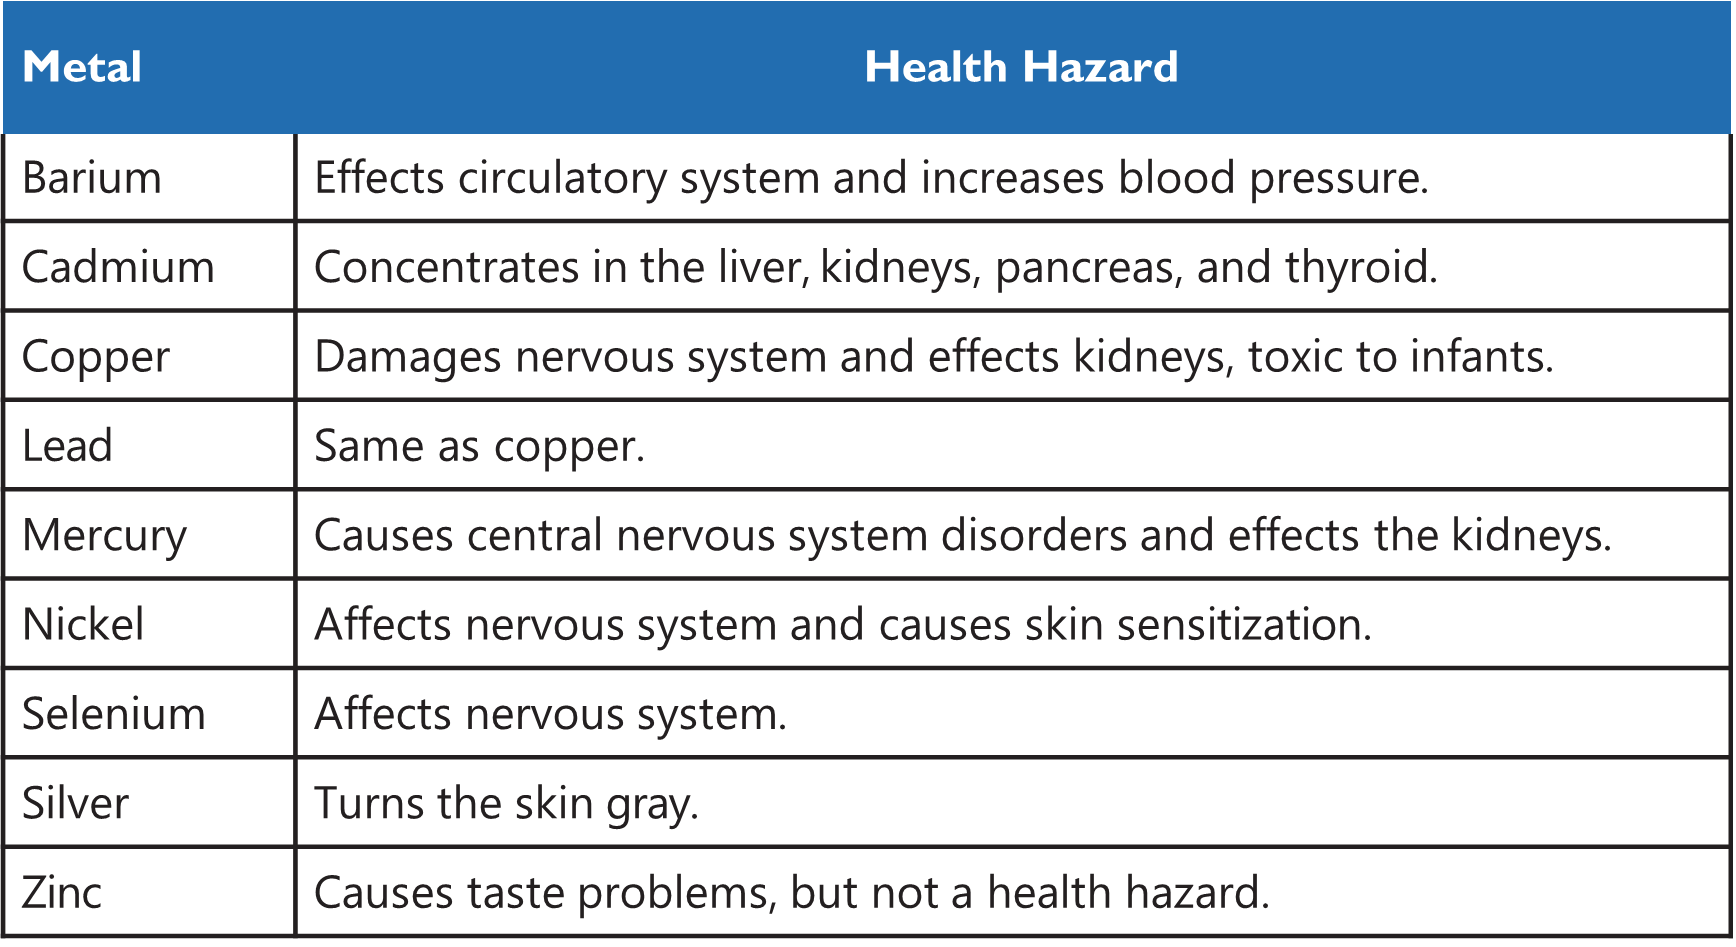
\includegraphics[scale=0.75]{MetalHealthHazard}
\caption{Metals in drinking water - health hazards}\index{Metals!Health hazards}
\end{center}
\end{figure}
\subsection{Salts}\index{Salts}
\begin{itemize}
\item A salt is formed when a metal ion (cation - because it has a positive charge) combines with a nonmetal ion (anion - because it has a negative charge). For instance, when a metal like sodium combines with a non-metal ion like chloride to form sodium chloride, NaCl, or table salt. \index{Anion} \index{Cation}

\item Common metal anions and cations that combine to form salts which are commonly found in drinking water supplies or used in Water treatment are listed in the table below.
\end{itemize}

\begin{table}[h!]    
\begin{center}
     \begin{tabular}{ | m{5cm}  m{5cm} |}
     \hline
           \multicolumn{1}{|c}{} & \multicolumn{1}{c|}{} \\
      \multicolumn{1}{|c}{\textbf{METAL ION (CATION)}} & \multicolumn{1}{c|}{\textbf{NON-METAL ION (ANION)}} \\
            \multicolumn{1}{|c}{} & \multicolumn{1}{c|}{}\\
      Calcium - Ca$^{+2}$ & Carbonate - CO$_3^{\enspace -1}$\\
      Magnesium - Mg$^{+2}$ & Bicarbonate - HCO$_3^{\enspace -1}$\\
      Manganese - Mn$^{+2}$ & Hydroxide - OH$^{-1}$\\
      Iron - Fe$^{+2/+3}$ & Sulfate - SO$_4^{\enspace -2}$\\
      Aluminum - Al$^{+3}$ & Chloride - Cl$^{-1}$\\
      Sodium - Na$^{+1}$ & \\
      Copper - Cu$^{+2/+3}$ & \\
          \hline
                    \end{tabular}
     \caption{Salts constituents}
     \label{Salts constituents}\index{Salts constituents}
     
\end{center}
     \end{table}

\begin{table}[h!]    
\begin{center}
     \begin{tabular}{ | m{5cm}  m{4cm}  m{4cm} |}
     \hline
           \multicolumn{1}{|c}{} & \multicolumn{1}{c}{} & \multicolumn{1}{c|}{}\\
      \multicolumn{1}{|c}{\textbf{CHEMICAL NAME}} & \multicolumn{1}{c}{\textbf{FORMULA}} & \multicolumn{1}{c|}{\textbf{COMMON NAME}}\\
            \multicolumn{1}{|c}{} & \multicolumn{1}{c}{} & \multicolumn{1}{c|}{}\\
      Aluminum sulfate & Al$_2$(SO$_4$)$_3$ & Alum\\
      Calcium oxide & Ca$ $O$ $ $ $ & Quicklime\\
      Calcium hydroxide & Ca$ $(OH$ $)$_2$ & Slaked/hydrated lime\\
      Calcium carbonate & Ca$ $CO$_3$ $ $ & Limestone\\
      Calcium hydroxide & Ca$ $(OH$ $)$_2$ & Slaked/hydrated lime\\
      Magnesium carbonate & Mg$ $(CO$_3$)$_2$ & \\
      Magnesium bicarbonate & Mg$ $(HCO$_3$)$_2$ & \\
      Sodium hydroxide & Na$ $OH$ $ $ $ & Caustic soda\\
      Sodium carbonate & Na$_2$CO$_3$ $ $ & Soda ash\\
      Ferrous sulfate & Fe$ $SO$_4$ $ $ & Copperas \\
      Ferric chloride & Fe$ $Cl$_3$ $ $ & \\
      Ferrous chloride & Fe$ $Cl$_2$ $ $ & \\
      Copper sulfate & Cu$ $SO$_4$ $ $ &\\

          \hline
                    \end{tabular}
     \caption{Salts found in water and/or used in water treatment}
     \label{Salts found in water and/or used in water treatment}\index{Salts found in water and/or used in water treatment}
     
\end{center}
     \end{table}

\subsection{Nutrients}\index{Nutrients}
\begin{itemize}
\item Plant nutrients - nitrogen and phosphorous\index{Nutrients!Nitrogen and phosphorous}, present in water promote growth of plant and algal matter in the receiving waters causing destruction of the normal aquatic life mainly due to oxygen depletion - eutrophication\index{Eutrophication}.
\item Major sources of nitrogen include runoff from animal feedlots, fertilizer runoff from agricultural lands, municipal wastewater discharges, and certain bacteria and blue-green algae than can obtain nitrogen directly from the atmosphere In addition,certain forms of acid rain can also contribute nitrogen to surface waters. Nitrogen in water is commonly found in the form of nitrate (NO$_3^{\enspace-}$) \index{Nitrates}
\item Nitrate in drinking water can lead to serious problems, specifically nitrate poisoning which can lead to death. Bacteria commonly found in the intestinal tract of infants can convert nitrate to highly toxic nitrites (NO$_2^{\enspace-}$). Nitrite can replace oxygen in the bloodstream and result in oxygen starvation, which causes a bluish discoloration of the infant known as infant methemoglobinemia or blue-baby syndrome \index{Infant methemoglobinemia or blue-baby syndrome}.  High nitrate levels may also affect the oxygen-carrying ability of the blood of pregnant women.
\item Nitrifying bacteria present in biological slime in the distribution system convert ammonia and other nitrogen compounds into nitrite (NO$_2$ $^-$) and then nitrate (NO$_3^{\enspace-}$).  This process is called nitrification. \index{Nitrification}
\item Major sources of phosphorous include phosphates in detergents, fertilizers and feedlot runoff, as well as municipal wastewater discharges.
\item Phosphate is added as part of the water treatment for corrosion control and for improving taste and odor by sequestering iron and magnesium.

\end{itemize}

\section{Trace constituents} \index{Trace constituents}
\begin{itemize}
\item Trace Constituents are chemicals found in extremely low concentrations.
\item Trace constituents include:
\begin{itemize}
\item B - Boron
\item Miscellaneous metals
\item Hormones
\item EDCs - Endocrine-disrupting compounds are synthetic and natural compounds that mimic, block, stimulate, or inhibit natural hormones in the endocrine systems of animals, including humans. The origins include pesticides, pharmaceutically active chemicals (PhACs), personal care products (PCPs), herbicides, industrial chemicals, and disinfection byproducts (DBPs).
\item PCPs - Personal Care Products are products such as shampoo, hair conditioner, deodorants, and body lotion.
\item Pharmaceuticals - aspirin, ibuprofen, caffeine, etc.
\item CECs - Constituents of Emerging Concern is a general term applied to constituents that have relatively recently become known as a potential concern and likely have little to no information available to fully comprehend and establish safe and realistic standards, such as PFAS/PFOA \index{PFAS/PFOA}.
\index{Trace constituents!Boron, hormones, EDCs, PCPs, CECs, PFAS/PFOA}
\end{itemize}
\end{itemize}

\section{Radionuclides}\index{Radionuclides}
\begin{itemize}
\item Radioactive materials, also called radionuclides, are both naturally occurring and human-made.

\item Radionuclides such as radium, radon and uranium can get into groundwater and surface waters from natural sources and also potentially from human sources such as active nuclear power plants or other facilities that make or use radioactive substances.

\item When radionuclides break down (decay), they emit radioactive particles such as alpha-particles, beta-particles and gamma-rays radiation which could present a risk to human health.

\item Most water systems have no detectable radionuclide activities, some areas of the United
States have significantly higher levels than the national averages.

\item People who are exposed to relatively high levels of radionuclides in drinking water for long periods may develop serious health problems, such as cancer, anemia, osteoporosis, cataracts, bone growths, kidney disease, liver disease and impaired immune systems.

\item The health risks associated with radionuclides are normally small compared with the risks from microorganisms and chemicals that may be present in drinking-water. 

\item The amount of radionuclides in drinking water is quantified and regulated under the EPA's Radionuclide Rule, by standards based upon both, the radioactivity levels as measured by the radiation of alpha and beta particles and the amount of commonly found radioactive elements - radium and uranium, quantified in terms of their radioactivity.
\item For drinking water, radiation/radioactivity levels is measured as pCi/L (picocuries per liter)\index{Radionuclides!Measurement!picocuries per liter (pCi/L)}
\end{itemize}



\section{Microbial contaminants}\index{Microbial contaminants}
\begin{itemize}
\item Many types of \textbf{pathogenic} - disease-causing germs can be found in contaminated drinking water, including bacteria, viruses and parasites.

\item Common virus in drinking water \index{Pathogens!Viruses} source and their associated diseases include:
\begin{itemize}
\item Adenoviruses - tonsillitis, conjunctivitis, the common cold and other illnesses. 
\item Reoviruses - colds, flu, diarrhea, chicken pox, measles and mumps.
\item polioviruses - polio
\item hepatitis A virus
\end{itemize}

\item Some of the water borne pathogenic bacteria \index{Pathogens!Bacteria} and their associated disease include:
\begin{itemize}
\item Salmonella typhi - Typhoid fever
\item Vibrio cholerae - cholera
\item Yersinia enterocolitica - gastroenteritis
\end{itemize}

\item Common intestinal parasites and their associated disease include \index{Pathogens!Parasites}:
\begin{itemize}
\item Entamoeba histolytica - Amoebic Dysentery.
\item Giardial lamblia (Giardiasis) \index{Pathogens!Parasites!Giardia}.
\item Ascaris lumbricoides (Giant Roundworm).
\item Cryptosporidium (Cryptosporidiosis) \index{Pathogens!Parasites!Cryptosporidium}.
\end{itemize}


\end{itemize}
 



\section{Physicochemical tests} \index{Physicochemical tests}

\begin{itemize}
\item The aesthetic quality \index{Aesthetic quality} aspects of drinking water include: taste, odor, color, turbidity, hardness, and temperature.
\item The aesthetics are generally not health-related. However, consumers can easily detect them, so they can have significant effects on perceptions of water quality and acceptability.
\item These attributes are the source of most complaints to water suppliers and frequently lead consumers to choose home treatment or bottled water.
\end{itemize}
\subsection{Turbidity}\index{Turbidity}
\begin{itemize}
\item Measures cloudiness of water due to suspended particles.
\item Higher turbidity levels are often associated with higher levels of disease-causing microorganisms.
\item Turbidity affects both the acceptability of water to consumers
\item Harmful pollutants such as heavy metals and pesticides are easily absorbed by suspended solids
\item Turbidity affects disinfection as suspended particles in water act as a protective shield for micro-organisms and provide an excellent substrate for bacteria growth.  Higher disinfection doses or contact times are required to ensure adequate treatment.
\item Suspended solids represent a risk for the main water distribution systems, pumps and other equipment where tend to deposit and block pipes and nozzles.
\item Turbidity is an optical measurement of water's ability to scatter and absorb light rather than transmit it in straight lines.  It is commonly measured in the unit of Nephelometric Turbidity Units (\textbf{NTU}). \index{Nephelometric Turbidity Units (NTU)}
\item "Crystal-clear” water has a turbidity of <1 NTU; at 4 NTU and above, water becomes visibly cloudy at 25 NTU it is murky.
\item An average person is able to see turbidity with the naked eye at NTU level of 5 and above.
\item Sources of turbidity:
\begin{enumerate}
\item In source water, turbidity can be attributed to:
\begin{itemize}
\item Inorganic particles released by weathering of rocks, soils and clays
\item Human, livestock and industrial wastes
\item Biological growth (e.g. algae, zooplankton and cyanobacteria) in source waters
\item Natural organic matter including decomposing plant material
\end{itemize}
\item Introduction of turbidity during treatment can be due to:
\begin{itemize}
\item Poor control of treatment chemical dosing (e.g. coagulants, settling aids and pH adjustment chemicals)
\item Precipitates from insoluble components of treatment chemicals, or formed during processes such as pH correction
\item Oxidation products of natural chemicals such as arsenic, iron and manganese
\end{itemize}
\item Turbidity can also be introduced in the distribution system by: \index{Turbidity}
\begin{itemize} 
\item Intrusion of soils and sewage through mains breaks
\item External contamination from backflow or cross connections
\item Resuspension of accumulated silts and sediments, or detachment of corrosion chemicals and scales and detachment of biofilms
\end{itemize}
\end{enumerate}
\item Formazin \index{Formazin} - a chemical, is used for preparing solutions of known turbidities.
\end{itemize}

\subsection{Color}\index{Color}
\begin{itemize}
\item Color may affect the turbidity value but is distinct from turbidity as color is due to organic material that has dissolved into solution, while turbidity consists of tiny particles suspended in the water column.
\end{itemize}

\subsection{Taste and odor}\index{Taste and odor}
\begin{itemize}
\item Odor and taste are useful indicators of water quality even though odor and taste-free water is not necessarily safe to drink nor water with some odors or taste is necessarily harmful.
\item Taste and odors are often grouped with odor because of their common origin factors. 
\item The cause of taste and odor issues can be from water fixtures, plumbing materials, water heaters, water treatment, pressure tanks and/or the source (the well).
\item Taste and odors are generally attributed to the presence of organic and some inorganic chemicals which come from the decaying organic matter, runoffs, industrial wastes, and municipal sewage discharges. 
\item Geosmin and methyl-isoborneol (MIB) are often the cause of earthy-musty odors occurring in fall due to the turnover of lakes and reservoirs.  They are produced by bacteria, particularly actinomycetes and cause odor issues at a very low concentrations.
\item In the groundwater, the tastes and odors can be due to iron, manganese, and hydrogen sulfide (H$_2$S).
\item Often, identifying the exact origin of taste and odor is usually very expensive and often impossible, and removal of the causative substance is even harder.
\item Current methods of measuring taste and odor are still fairly subjective.  Standards related to odor and taste: Chloride, Copper, Foaming Agents, Iron, Manganese pH, Sulfate, Threshold Odor Number (\textbf{TON})\index{Threshold odor number (TON)} which is the greatest dilution of a sample with odor-free water that still yields a just-detectable odor.
\end{itemize}

\subsection{Temperature}\index{Temperature}
\begin{itemize}
\item Temperature affects the solubility of oxygen in water, the rate of bacterial activity, and the rate at which gases are transferred to and from the water.
\item Cool water is generally more palatable than warm water, and temperature will have an impact on the acceptability of a number of other inorganic constituents and chemical contaminants that may affect taste. 
\item High water temperature enhances the growth of microorganisms and may increase problems related to taste, odor, color and corrosion.
\item Water temperature determines, in part, how efficiently certain water treatment processes operate. For example, temperature has an effect on the rate at which chemicals dissolve and react. When water is cold, more chemicals are required for efficient coagulation and flocculation to take place. When water temperature is high, the result may be a higher chlorine demand because of the increased reactivity, as well as an increased level of algae and other organic matter in raw water.
\item Heat is added to surface and groundwater from natural and man-made sources.  Surface waters in particular  are potentially subject to great temperature variations. 
\item Other sources of increased temperatures in running water result from forest clearing and return of irrigation flows to a body of running water.
\end{itemize}

\subsection{Total dissolved solids}\index{Total dissolved solids}
\begin{itemize}
\item Total dissolved solids (\textbf{TDS}) is a part of total solids (\textbf{TS}) in water and are the material remaining in water after filtration.
\item Components of water TDS include:
\begin{itemize}
\item Minerals from rocks and soil as water passes over and through them.
\item Pesticides and herbicides from agricultural runoff
\item Lead and copper from plumbing pipes
\item Chemicals added during water treatment
\item Human and animal wastes
\item Biological decay products
\end{itemize}
\item Water has an equilibrium state with respect to dissolved portion; thus, if water is under saturated, it will aggressively dissolve materials it comes into contact with. Because of this problem, certain soluble substances, typically calcium and magnesium based substances are added post water treatment to minimize its corrosivity effects in the distribution system.
\item Dissolved solids can be removed from water by distillation, electro-dialysis, reverse osmosis, or ion exchange.
\item TDS is measured in mg/L or ppm.  
\item As water will conduct electricity due to the presence of dissolved inorganic ions, higher the concentration of these ions, the higher is the conductivity. Thus, specific conductance \index{Specific conductance} - conductivity measurement, provides a good estimate of the water's TDS.
\item The terms “specific conductance,” “specific electrical conductance,” and
“electrical conductivity” are used interchangeably and its unit of measurement is in Siemens per centimeter (S/cm) or mhos per centimeter (mhos/cm) \index{mhos per centimeter (mhos/cm)} \index{Siemens per centimeter (S/cm)}.
\item The TDS concentration is considered a Secondary Drinking Water Standard, which means that it is not a health hazard.
\item EPA has established a Secondary Drinking Water Standard of a maximum concentration of 500 mg/l of TDS \index{Total dissolved solids!Secondary standard}in drinking water and  recommends treatment when TDS concentrations exceed 500 mg/L, or 500 parts per million (ppm). 
\end{itemize} 

\subsection{pH}\index{pH}	
			pH is a measure of the hydrogen ion (H$^+$) content or the acidity or basicity of a solution.  pH impacts the chemical and microbiological elements of water treatment processes and thus pH measurement and control is critical.
			\begin{itemize}
				\item Pure water dissociates into equal concentration of hydrogen ions and hydroxide ions:\\ 
				      $H_2O \rightarrow H^+ + OH^-$.
				\item The H$^+$ are responsible for acidic properties and the OH$^-$ ions for the basic properties.  
				\item pH is the inverse of H$^+$ concentration; pH increases when the concentration of H$^+$ decreases relative to the concentration of OH-. 
				\item pH scale ranges from 0 – 14. When the concentration of both H$^+$ and OH$^-$ are equal, as in pure water, it is considered neutral and its pH is 7.0.  \item If the pH of a sample solution is below 7.0, the sample is termed acidic and is alkaline or basic if its pH is above 7.0. 
				\item Each change of 1 pH unit represents a 10 fold change in concentration.  For example, a sample with a pH of 2.0 is 1000 times more acidic than a sample with a pH of 5.0.
				
				\item The affects of drinking water pH include:
				\begin{itemize}
				\item Taste and odor impacts.
				\item Solubility and biological availability of chemical constituents such as nutrients - phosphorus, nitrogen, and carbon.
				\item Solubility and toxicity of heavy metals.  Metals tend to be more toxic at lower pH because they are more soluble.
				\end{itemize} 
				\item pH is measured by an electrode that is sensitive only to H$^+$ or using a pH strip which is essentially an adsorbent paper which is pre-impregnated with chemicals which change color under different H$^+$ concentrations.
						
\item \index{pH!pH measurement}It is important to measure pH at the same time as chlorine residual since the efficacy of disinfection with chlorine is highly pH-dependent; where the pH exceeds 8.0, disinfection is less effective. To check that the pH is in the optimal range for disinfection with chlorine (less than 8.0), simple tests may be conducted in the field using comparators such as that used for chlorine residual. With some chlorine comparators, it is possible to measure pH and chlorine residual simultaneously.

\item Alternatively, portable pH electrodes and meters are available. If these are used in the laboratory, they must be calibrated against fresh pH standards at least daily; for field use, they should be calibrated immediately before each test. Results may be inaccurate if the water has a low buffering capacity.
\end{itemize}

\subsection{Alkalinity}\index{Alkalinity}
\begin{itemize}
\item Alkalinity is a measure of the ability of water to neutralize acid, or an expression of its buffering capacity.
\item Constituents of alkalinity are: Bicarbonate – HCO$_3$, Carbonate - CO$_3$ , Hydroxide - OH$^-$
\item Measured in equivalent of mg/L CaCO$_3$
\item Alkalinity levels can be classified as:
\begin{itemize}
\item Low Alkalinity - < 20 mg CaCO$_3$/L
\item Moderate Alkalinity - 20 to 160 mg CaCO$_3$/L
\item High Alkalinity - > 160 mg CaCO$_3$/L
\end{itemize}
\item High alkalinity indicates the scaling (deposit forming) potential and salty taste
\item Low alkalinity implies undersaturation of water (absence of dissolved content) and thus would exhibit higher corrosion potential - tendency to dissolve metals.
\item Alkalinity originates naturally as water moves through rocks dissolving minerals.
\item Alkalinity is important for fish and aquatic life because it protects or buffers against rapid pH changes. In addition, alkalinity levels affect the efficiency of certain water treatment processes, especially the coagulation process.
\end{itemize}


\subsection{Hardness}\index{Hardness}
\begin{itemize}
\item Hardness is due to the presence of multivalent metal ions, which come from minerals dissolved in water.  The dissolution of these minerals is aided by the carbonic acid formed by the dissolution of naturally occurring carbon dioxide in water. 
\item Domestic use of hard water is marked by lack of foam formation with soap solutions due to the formation of a white precipitate (soap scum) instead of producing lather and formation of noticeable limescale in kettles and water heaters.
\item Calcium (Ca) and Magnesium (Mg) \index{Calcium} \index{Magnesium} are the two metals that dissolve the most easily in water. They are considered to be the main cause of hardness.
\item Hardness causing compounds are broken into two groups:\\
\begin{itemize}
\item \ul{Carbonate hardness or temporary hardness} \index{Carbonate hardness or temporary hardness}which is the hardness that can be removed by boiling water.
\begin{itemize}
\item Carbonate hardness is formed when calcium or magnesium combines with a form of alkalinity (carbonate, bicarbonates, or hydroxides.) 
\end{itemize}
\item \ul{Non-carbonate hardness} \index{Hardness!Carbonate hardness} cannot be removed by boiling water.
\begin{itemize}
\item Non-carbonate hardness \index{Hardness!Non-carbonate hardness}is formed when calcium and magnesium combine with anything other than alkalinity. Chlorides and sulfates are the two most common forms of non-carbonate hardness.
\end{itemize}
\end{itemize}
\item Hard water when used in industrial applications forms deposits - scale composed mainly of calcium carbonate (CaCO$_3$), magnesium hydroxide (Mg(OH)$_2$), and calcium sulfate (CaSO$_4$)on the inside surfaces of pipes and heat exchangers. The scale formed restricts the flow of water, heat transfer causing metal boiler components to overheat.
\item Water hardness has not be found to cause adverse health effects in humans.  
\item Generally speaking, groundwaters are harder than surface waters.  In freshwater, the primary ions are calcium and magnesium; however, iron and manganese may also contribute. 
\item Hardness is classified as carbonate hardness or non carbonate hardness. Carbonate hardness is equal to alkalinity but a non-carbonate fraction may include nitrates and chlorides.
\item Hardness of water is determined by titrating with a standard solution of ethylene diamine tetra acetic acid (\textbf{EDTA}) \index{EDTA} which is a complexing agent \index{Hardness!Testing}.
\item Hardness values are expressed as an equivalent amount or equivalent weight of calcium carbonate in mg/l. 
\item Water with a hardness of less than 50 ppm is soft. Above 200 ppm, domestic supplies are usually blended to reduce the hardness value.
\item The \textbf{grain per gallon} \index{grain per gallon} is a unit of water hardness defined as 1 grain (64.8 milligrams) of calcium carbonate dissolved in 1 gallon of water. It translates into 17.1 parts per million (ppm).
\end{itemize}
\textit{Note: Alkalinity and hardness can be seen as two sides of the same coin.  Typical minerals found in water include - CaCO$_3$, Ca(HCO$_3$)$_2$, CaSO$_4$, MgCO$_3$, Mg(HCO$_3$)$_2$ - the cations of these minerals - Ca$^{+2}$ and Mg$^{+2}$ contribute to hardness while the anions - CO$_{3}^{-2}$,SO$_{4}^{-2}$ HCO$_{3}^{-}$ contribute to the alkalinity.  These dissolved minerals are measured as part of the TDS.  Thus, in natural waters - TDS, alkalinity and hardness are typically correlated.}




\subsection{Langelier index}\index{Langelier index}
\begin{itemize}
\item The Langelier Index is an approximate indicator of the degree of saturation of calcium carbonate in water. 
\item It is calculated using the pH, alkalinity, calcium concentration, total dissolved solids, and water temperature of a water sample collected at the tap.
\item The sign and magnitude of the Langelier index show the water’s tendency to form or dissolve scale and thus to inhibit or encourage corrosion:
\begin{itemize}
\item A negative Langelier Index indicates calcium carbonate under-saturation and water will have a higher corrosion potential.
\item Positive Langelier Index indicates  calcium carbonate over-saturation and indicates scaling potential of that water.
\item Water with a Langelier Index of close to zero, indicates water which is not corrosive nor scale forming.
\end{itemize}
\item Langelier index can be utilized to identify the water supply systems' leakage potential.
\end{itemize}

\subsection{Chlorine residual}\index{Chlorine residual}
\begin{itemize}
\item  Chlorine in one form or another is the principal disinfecting agent employed. 
\item An important additional advantage over some other disinfectants is that chlorine leaves a disinfectant residual that assists in preventing recontamination during distribution, transport, and household storage of water. 
\item The absence of a chlorine residual in the distribution system may, in certain circumstances, indicate the possibility of post-treatment contamination.
\item Three types of chlorine residual may be measured: 
\begin{enumerate}
\item \textbf{Free chlorine} \index{Chlorine disinfection!Free chlorine} - the most reactive form, which is the chlorine present as hypochlorite (OCl$^-$), hypochlorous (HOCl) or a combination of the two.  
\item \textbf{Combined chlorine} - the less reactive but more persistent form, consisting of chlorine that is combined with ammonia, nitrogen, or nitrogenous compounds (chloramines). This is the amount of chlorine that has reacted with nitrates and is unavailable for disinfection. 
\item \textbf{Total chlorine}\index{Chlorine disinfection!Total chlorine} - which is the sum of the free and combined chlorine residuals.
\end{enumerate}
\item Free chlorine is unstable in aqueous solution, and the chlorine content of water samples may decrease rapidly, particularly at warm temperatures. Also, exposure to strong light or agitation will accelerate the rate of loss of free chlorine. \textbf{Water samples should be analyzed for free chlorine immediately on sampling and not stored for later testing.}
\item \textbf{DPD} - N,N-diethyl-p-phenylenediamine \index{Chlorine disinfection!Chlorine measurement!DPD}, is a commonly used method of measuring the chlorine residual in water. DPD reacts directly with disinfectants (e.g. chlorine, chloramines etc.) to produce a pink colored solution. The intensity of this colored solution is proportional to the concentration of disinfectant in the sample.
\item Residual chlorine analysis of a water sample is preferably to be conducted immediately, but must be done within 15 minutes of sampling. 
\item Amperometric sensors \index{Chlorine disinfection!Chlorine measurement!Amperometric} are also used for chlorine measurements.  
\item Advantages of amperometric method include:
\begin{itemize}
\item Chemical reagents are not required
\item Sensors are relatively free from interference from color, turbidity, and interference from iron, manganese, nitrate and chromates present in the sample.
\end{itemize}
\end{itemize}

\subsection{Density}\index{Density}
\begin{itemize}
\item Density is defined as the weight of a substance per a unit of its volume. 
\item Density is typically measured in units of lb/ft$^3$, lb/gal, or mg/L. 
\item Density of water = 62.4 lb/ft$^3$ or 8.34 lb/gal.
\end{itemize}

\subsection{Specific gravity}\index{Specific gravity}
\begin{itemize}
\item Specific gravity is a relationship of the density of a particular liquid or solid to water. 
\item Specific gravity for any substance is calculated by dividing the weight of a certain volume of that substance to the weight of the same volume of  water.
\item A substance that is heavier than water will have a specific gravity greater than one and it will sink in water; if the specific gravity is less than one, it will float.
\item Specific gravity has no units. 
\item Specific gravity of water = 1.0 
\end{itemize}

\begin{table}[]
\centering
\begin{tabular}{|l|l|l|}
\hline
\multicolumn{1}{|c|}{\textbf{Substance}} & \multicolumn{1}{|c|}{\textbf{Density} }& \multicolumn{1}{|c|}{\textbf{Specific Gravity}}\\ \hline
Alum (8\% @60°F)                         & 11.1 lbs/gal     & \multicolumn{1}{|c|}{1.33 }                     \\ \hline
Hydrogen peroxide (35\%)                 & 9 lbs/gal        & \multicolumn{1}{|c|}{1.13 }                    \\ \hline
Concrete                                 & 130 lbs/ft$^3$      & \multicolumn{1}{|c|}{2.08 }                      \\ \hline
Iron                                     & 491 lbs/ft$^3$      & \multicolumn{1}{|c|}{7.85 }                     \\ \hline
\end{tabular}
\caption{Density and specific gravity examples}
\end{table}
\section{Microbial testing}\index{Microbial testing}
\begin{itemize}
\item It is not practical to monitor for every pathogen that may potentially be present in drinking water source, thus an “indicator organism approach” to assess the microbiological quality of drinking water is adopted.

\item “Coliform” bacteria-particularly Escherichia coli (better known as E. coli) are used as the indicator organisms.\index{Coliform bacteria}

\item These coliform bacteria originate from feces and indicate fecal contamination and thus serve as an indicator organisms for pathogens of wastewater origin
			\item They are also abundant, potentially less harmful, and easy to detect
\item The methods for water bacteriological tests include:  multiple-tube fermentation (MTF) technique, membrane filtration (\textbf{MF}), Presence - Absence Method,  and quanti-tray testing.  \item When using the MTF and MF methods, it is not possible to exactly quantify the number of bacteria present, a statistical based - Most Probable Number (\textbf{MPN}) approach is utilized\\
\end{itemize}
\subsection{Multiple-tube fermentation (MTF)}\index{Microbial testing!Multiple-tube fermentation (MTF)}
\begin{enumerate}[label={\bfseries Stage \arabic*}]
\item Presumptive Test:
\begin{enumerate}[Step 1.]
\item Multiple-Tube Fermentation (\textbf{MTF}) technique involves adding three volumes – 10 ml, 1 ml and 0.1 ml of the sample, each to a set of five tubes containing Lauryl Tryptose broth and an inverted tube (Durham tube), 
\item The tubes are incubated for 24 hours and after incubation the tubes are checked for positive results.  The Lauryl Tryptose broth produces color and/or turbidity change due to the growth of the target bacteria and the inverted tube collects the gas produced by the bacterial respiration.  
\end{enumerate}
\item Confirmed Test:
\begin{enumerate}[Step 1.]
\item Each positive is innoculated into bacteria specific broth and observed for positive results after incubating the innoculated samples for 24 hours.
\item The number of tubes showing bacterial growth are counted for each volume of sample and using this information the concentrations of organisms in the original sample are established using Statistical Tables.
\end{enumerate}
\item Completed Test:
\begin{enumerate}[Step 1.]
\item An innoculum from the Confirmed positive is streaked on agar plates and incubated
\item The colonies from the agar plate are innoculated on an agar slant and nutrient broth and incubated.
\item The above incubated samples are observed for positive results.
\end{enumerate}
\end{enumerate}
% \begin{landscape}
% \begin{center}
%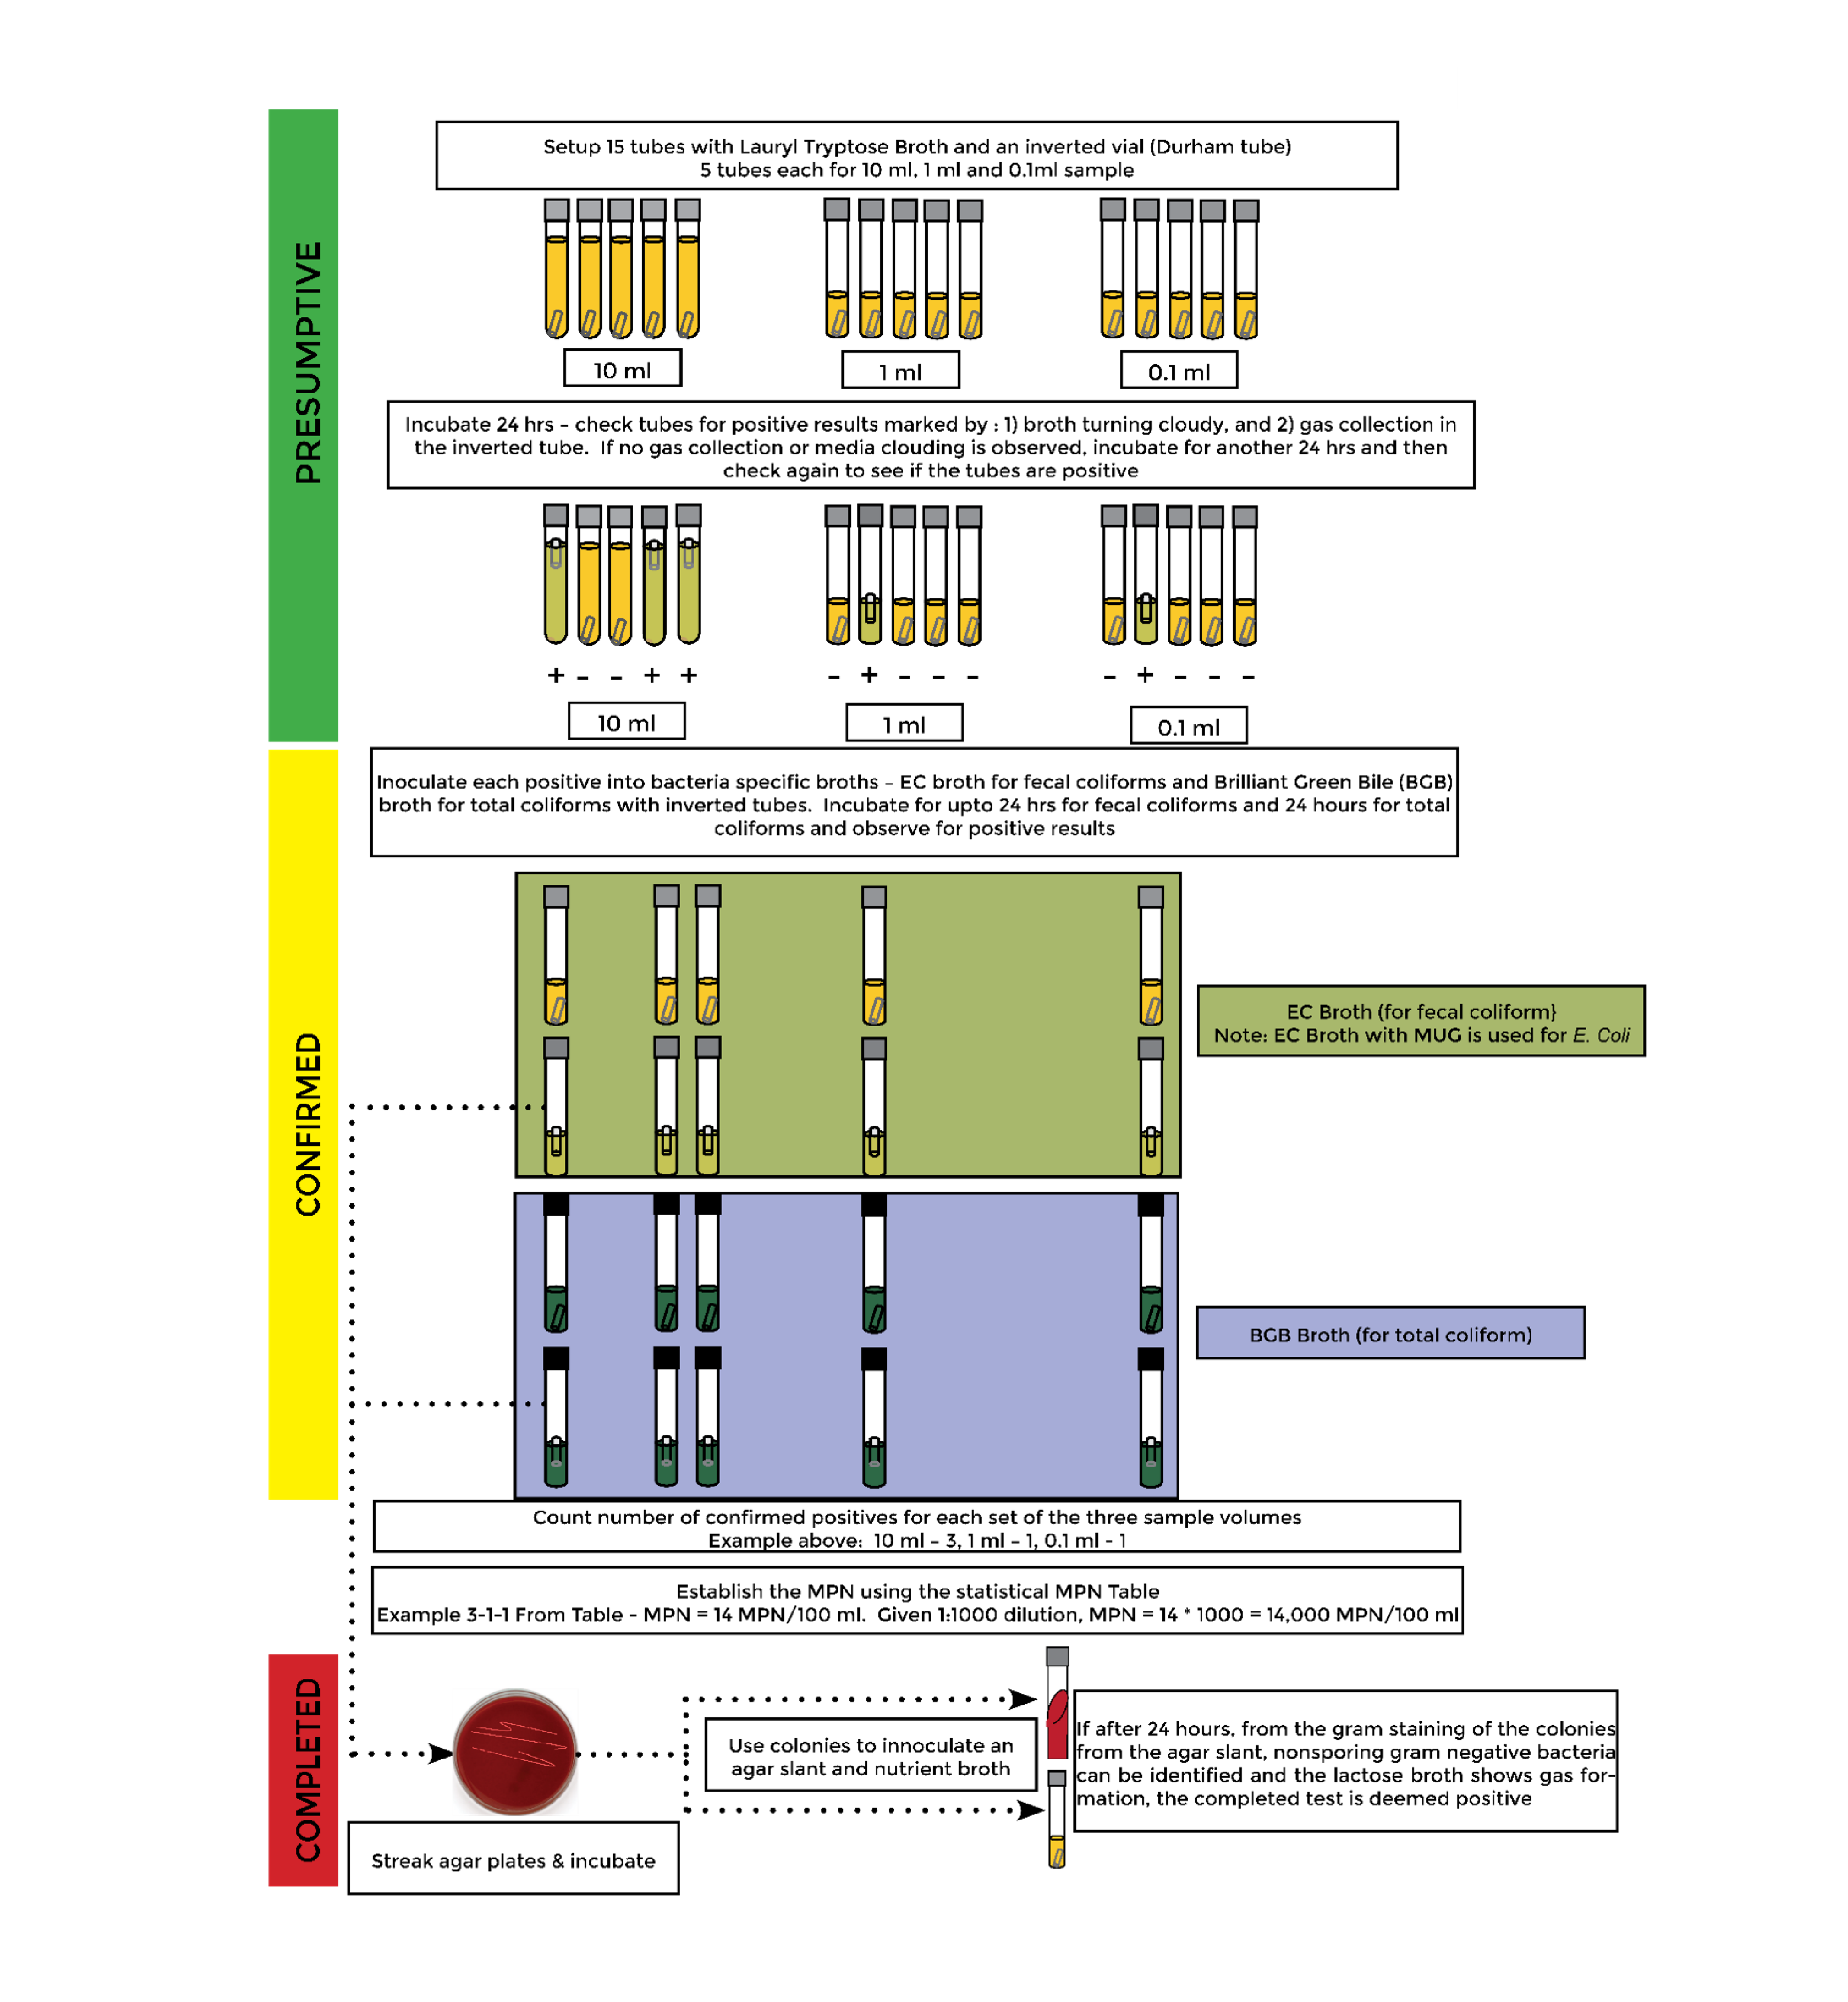
\includepdf[]{WaterMTF.pdf}
%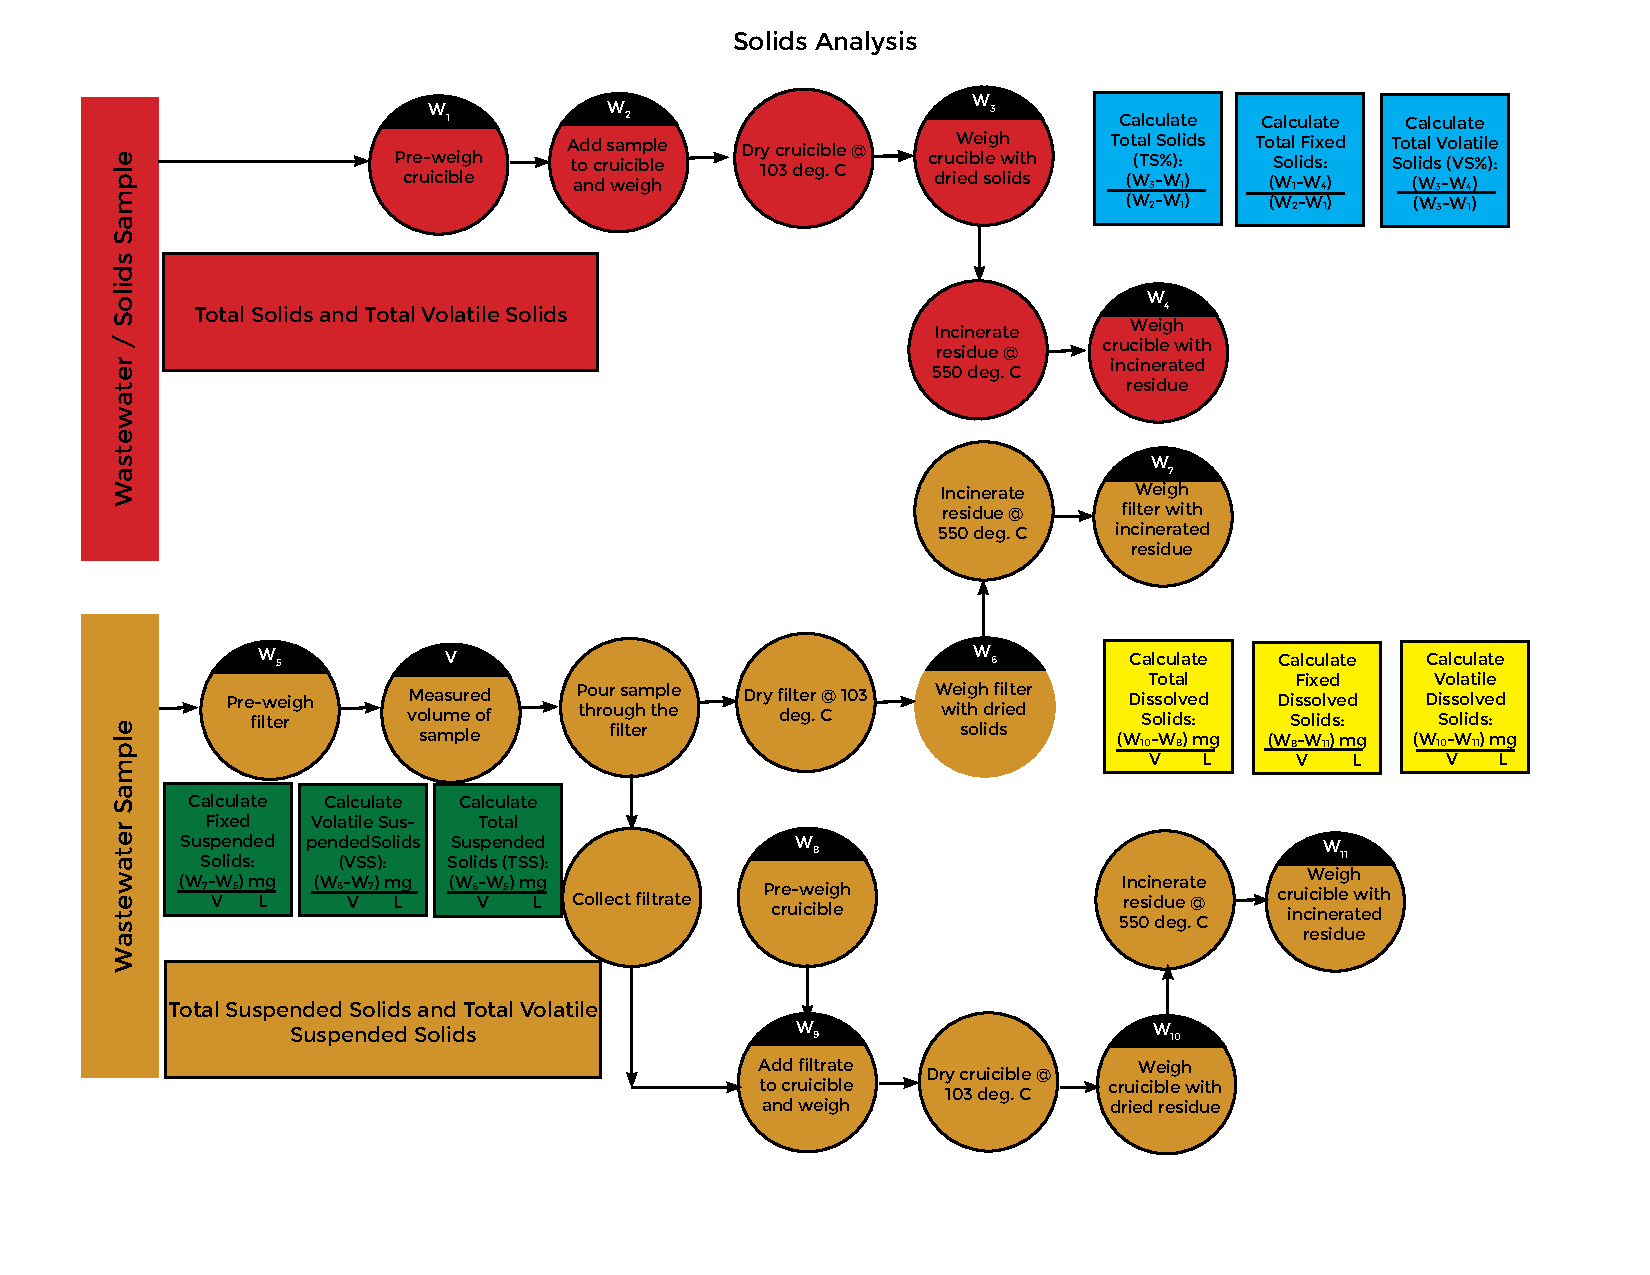
\includegraphics[scale=0.69]{LaboratorySolidsAnalysis4_01.pdf}
% \end{center}
% \end{landscape}
\begin{figure}[H]
\begin{center}
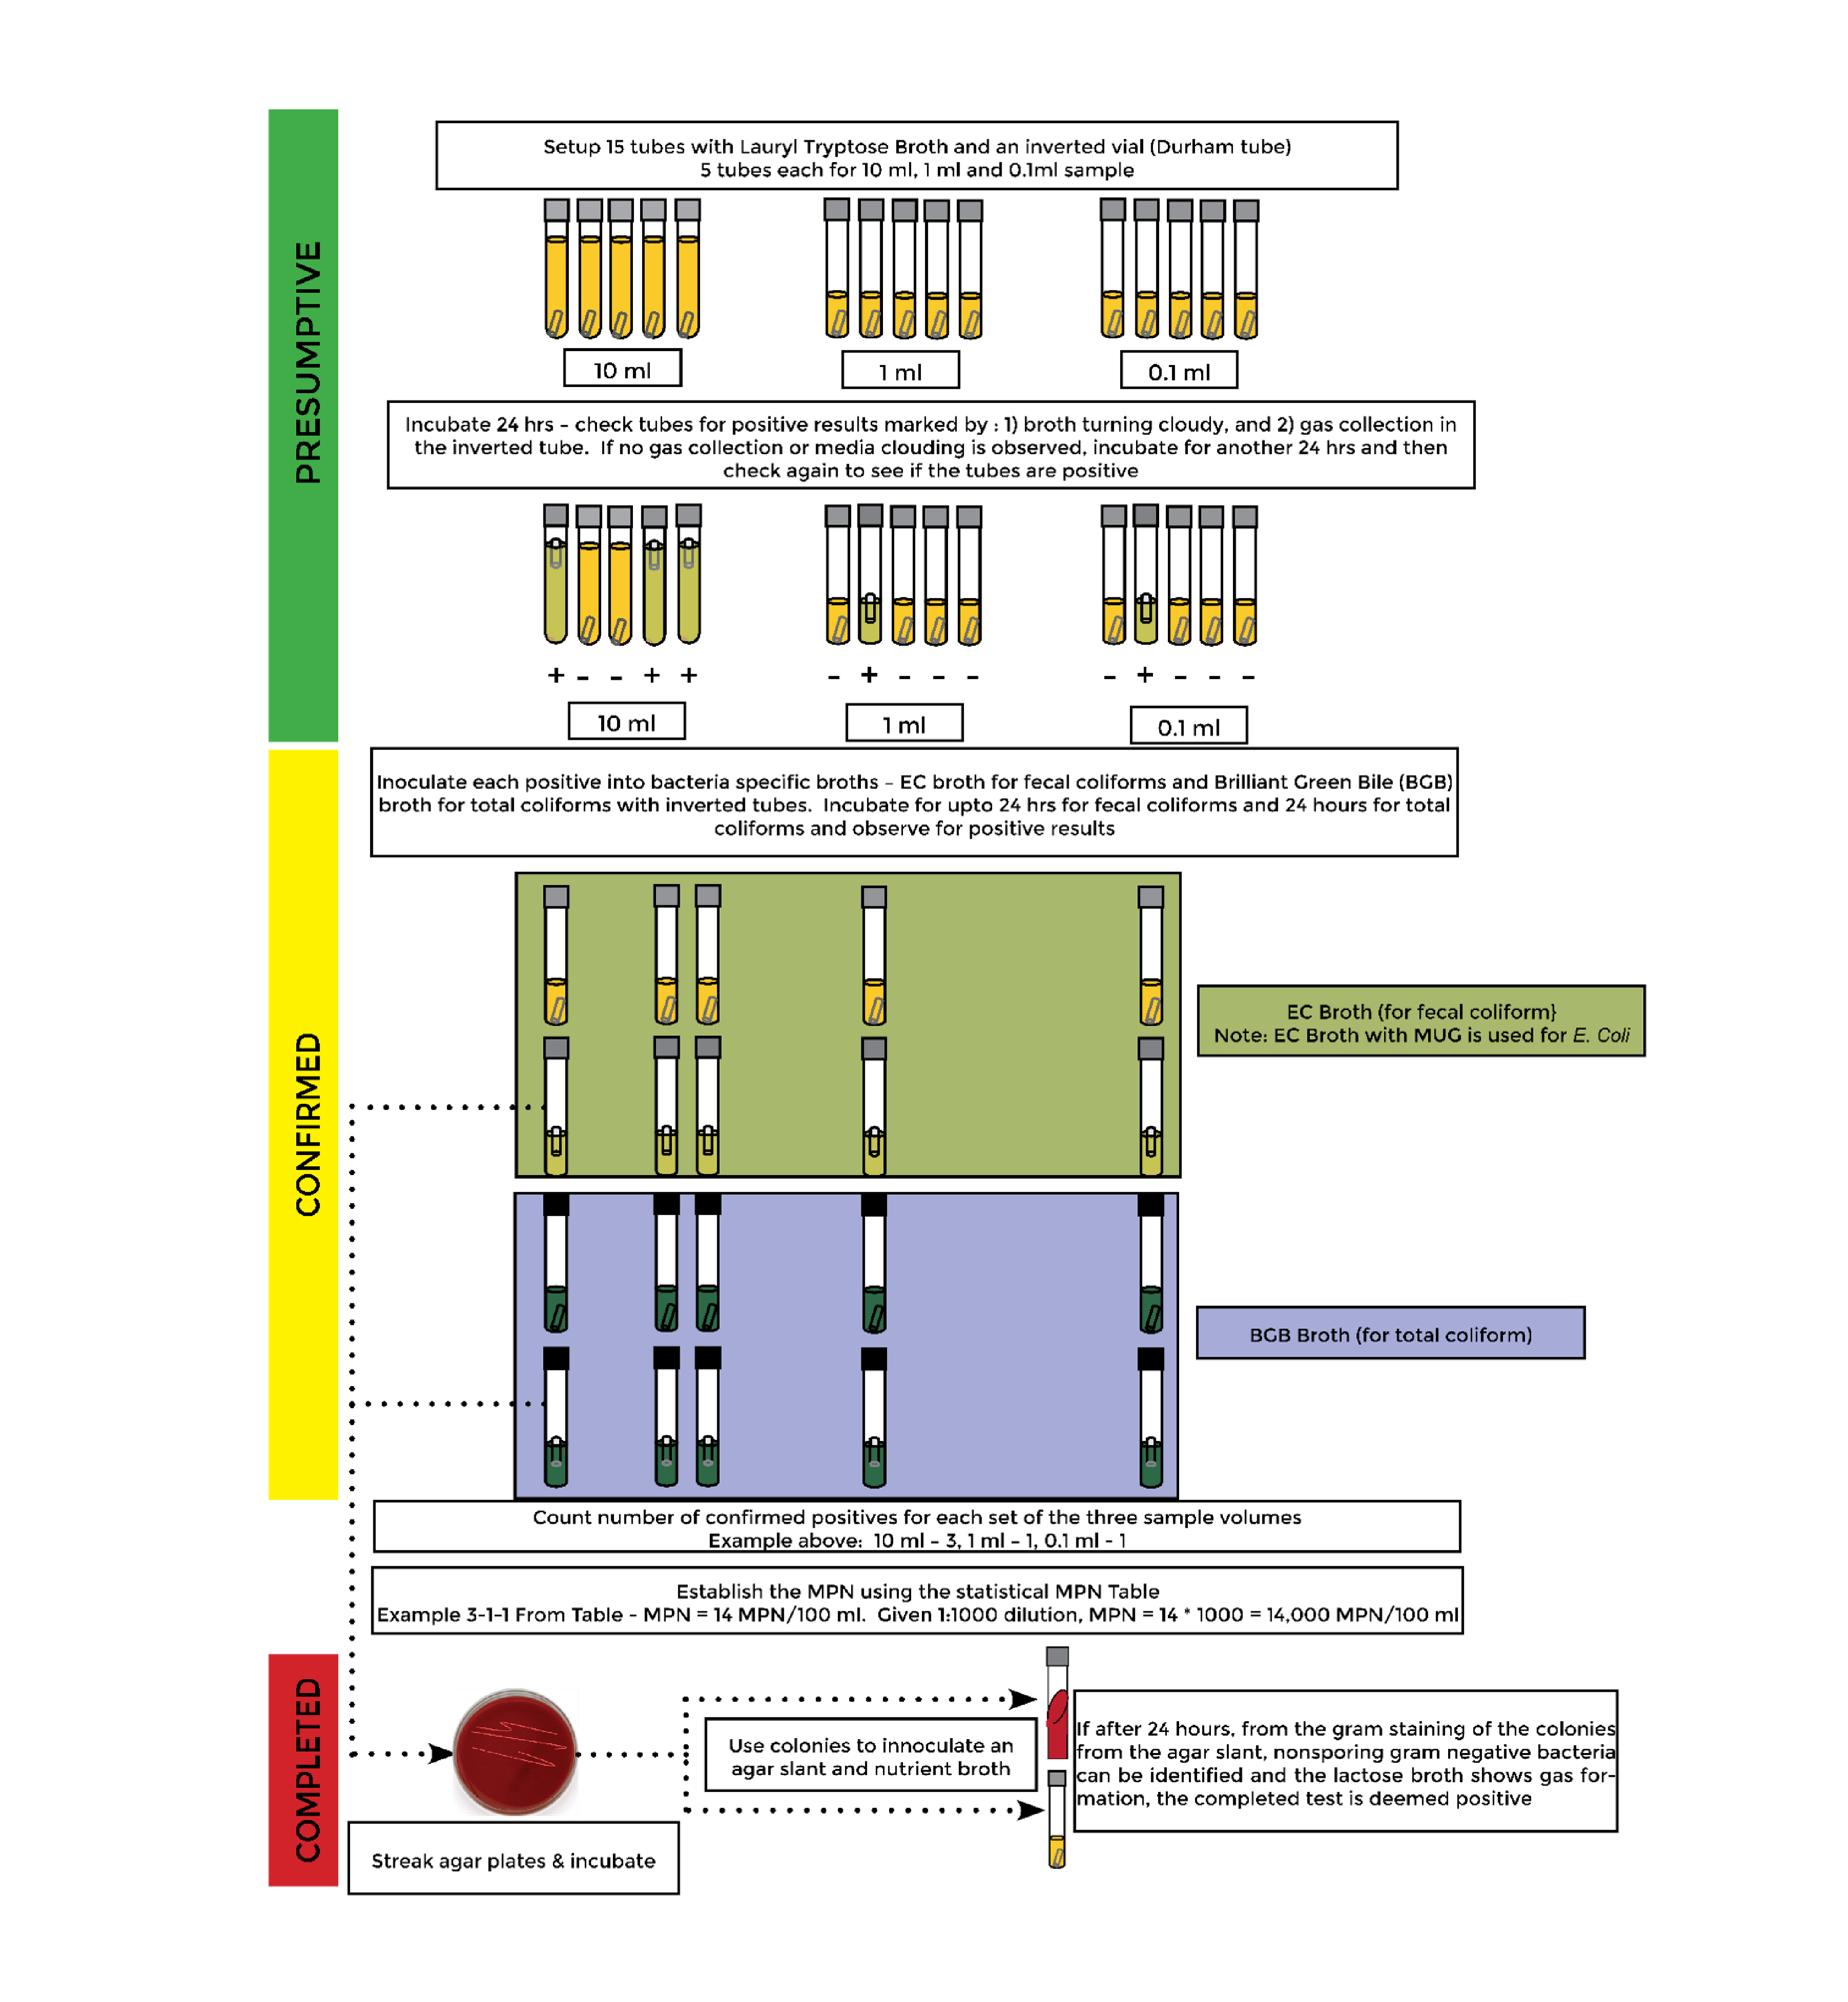
\includegraphics[scale=0.25]{WaterMTF}
\caption{Multiple tube fermentation}
\end{center}
\end{figure}
%\begin{figure}
%\begin{center}
%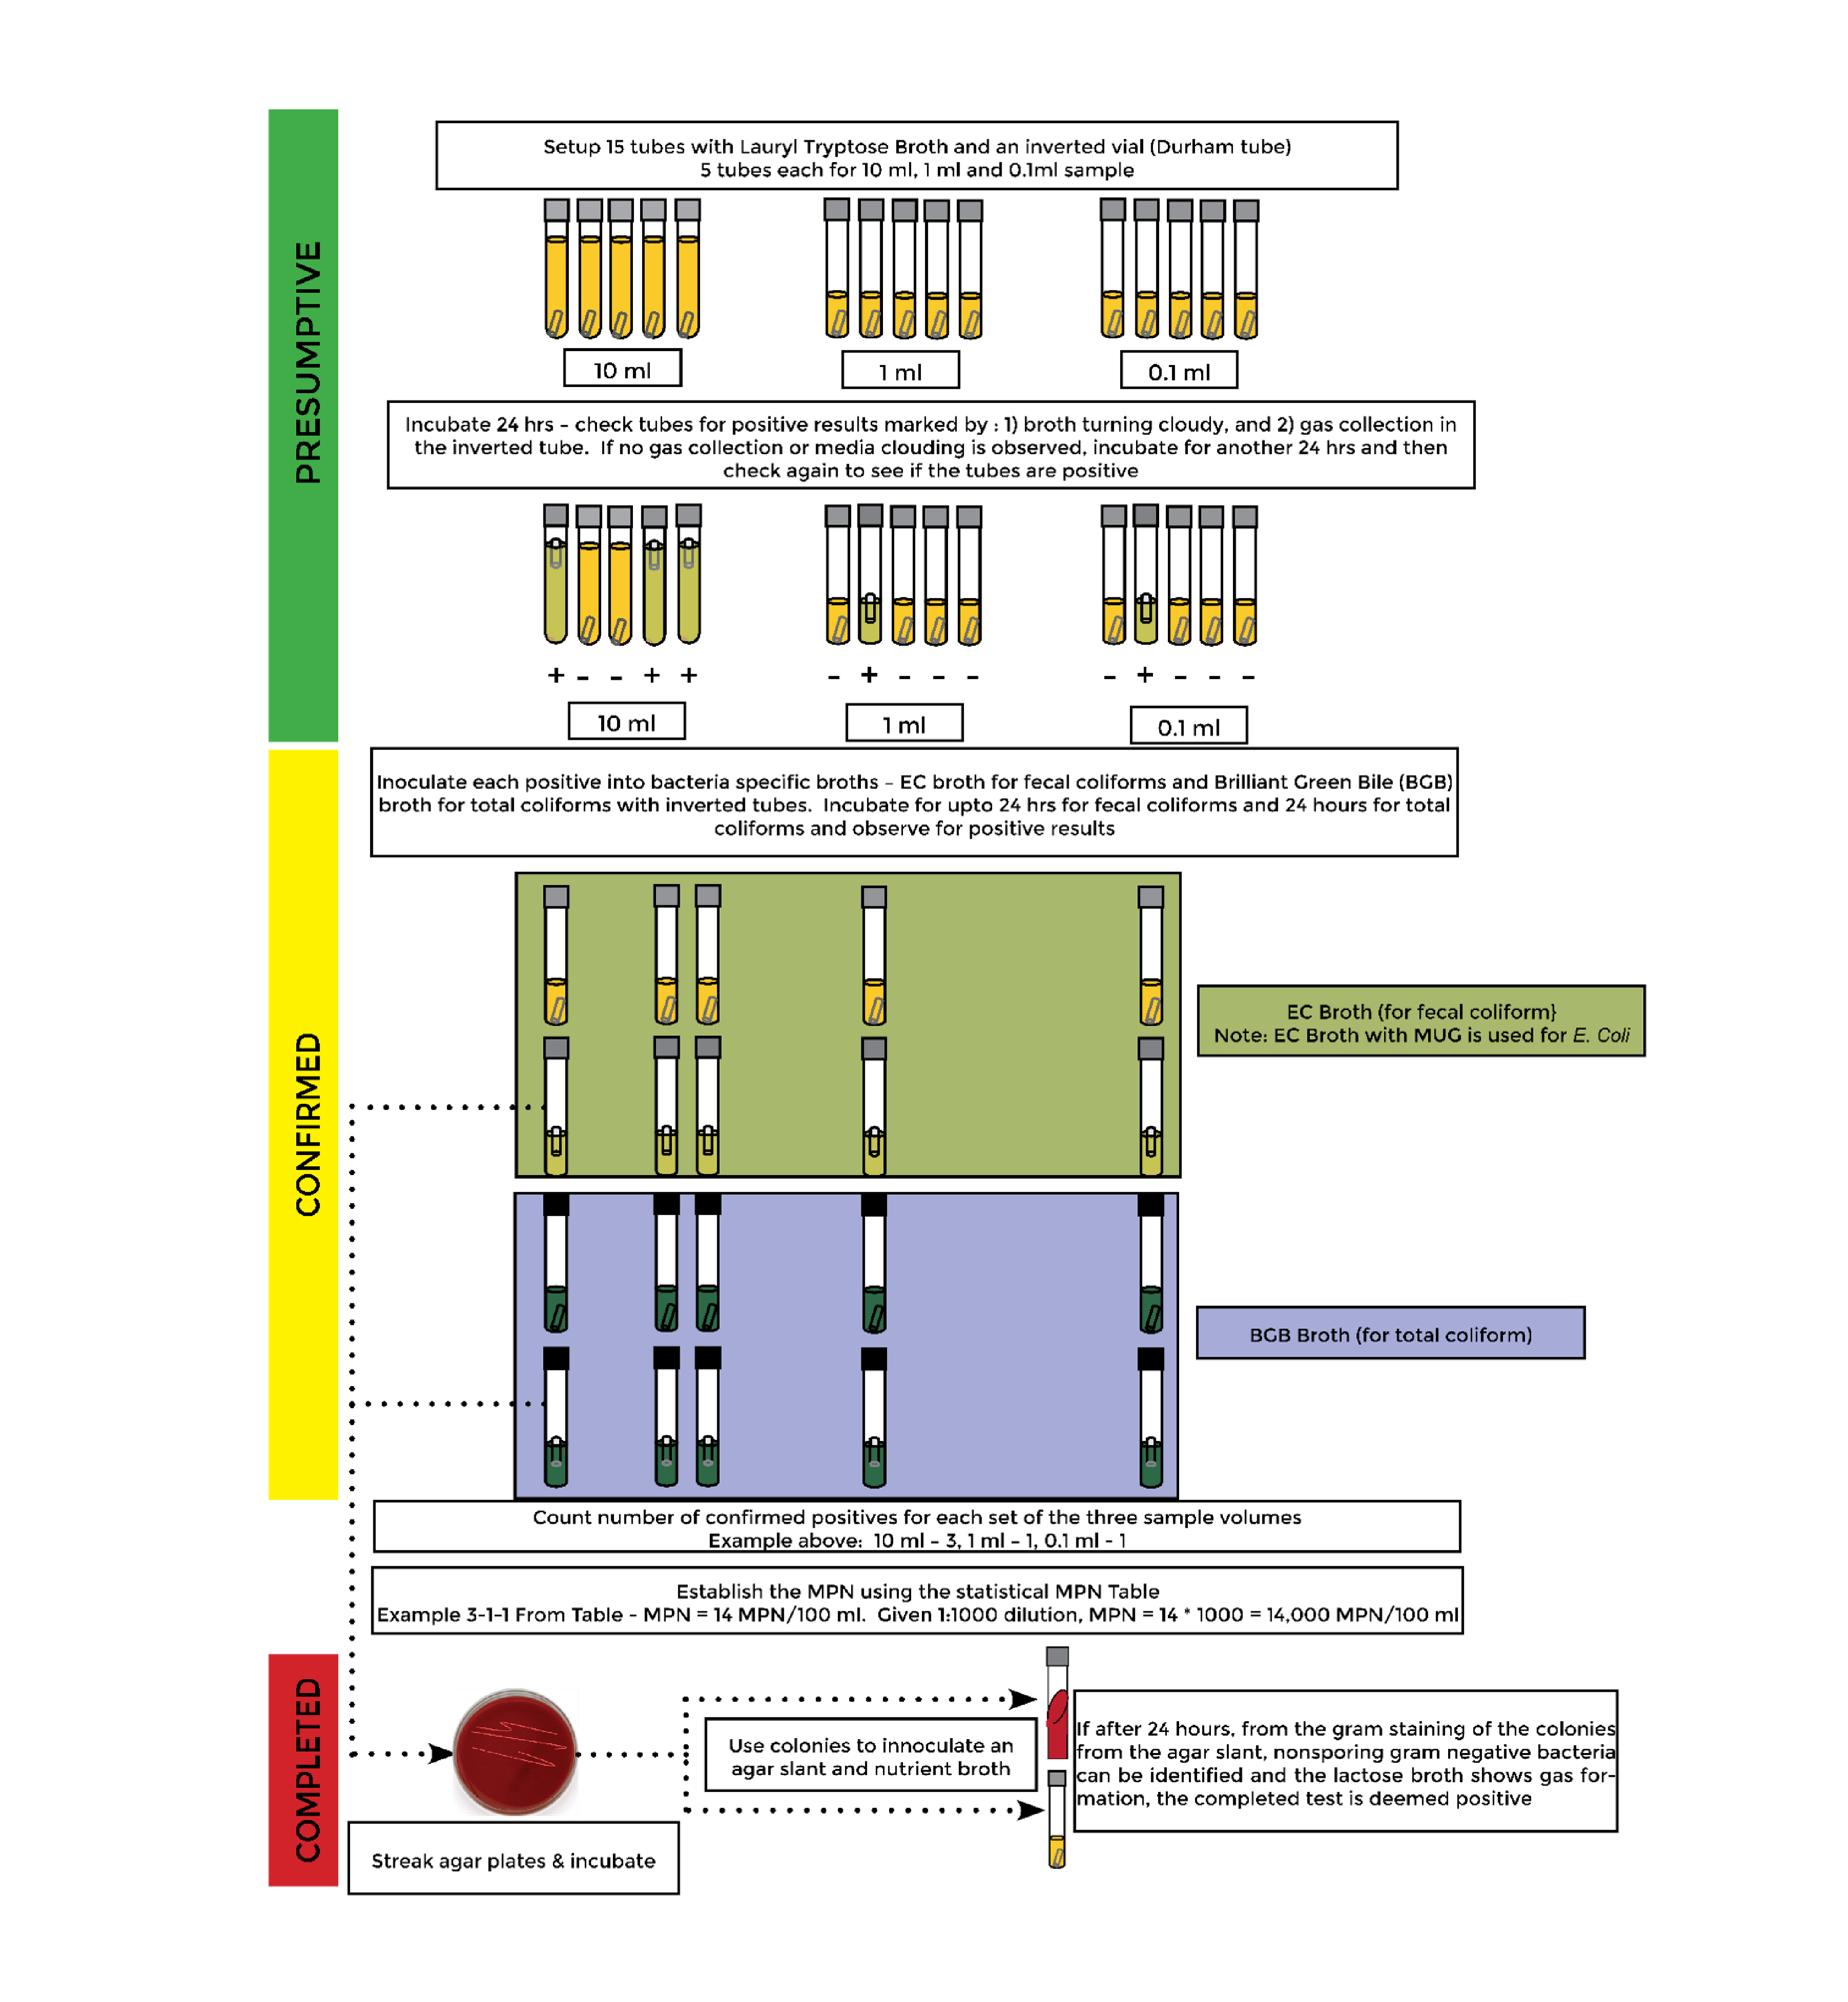
\includegraphics[scale=0.3]{WaterMTF}
%\end{center}
%\end{figure}
\thispagestyle{empty}
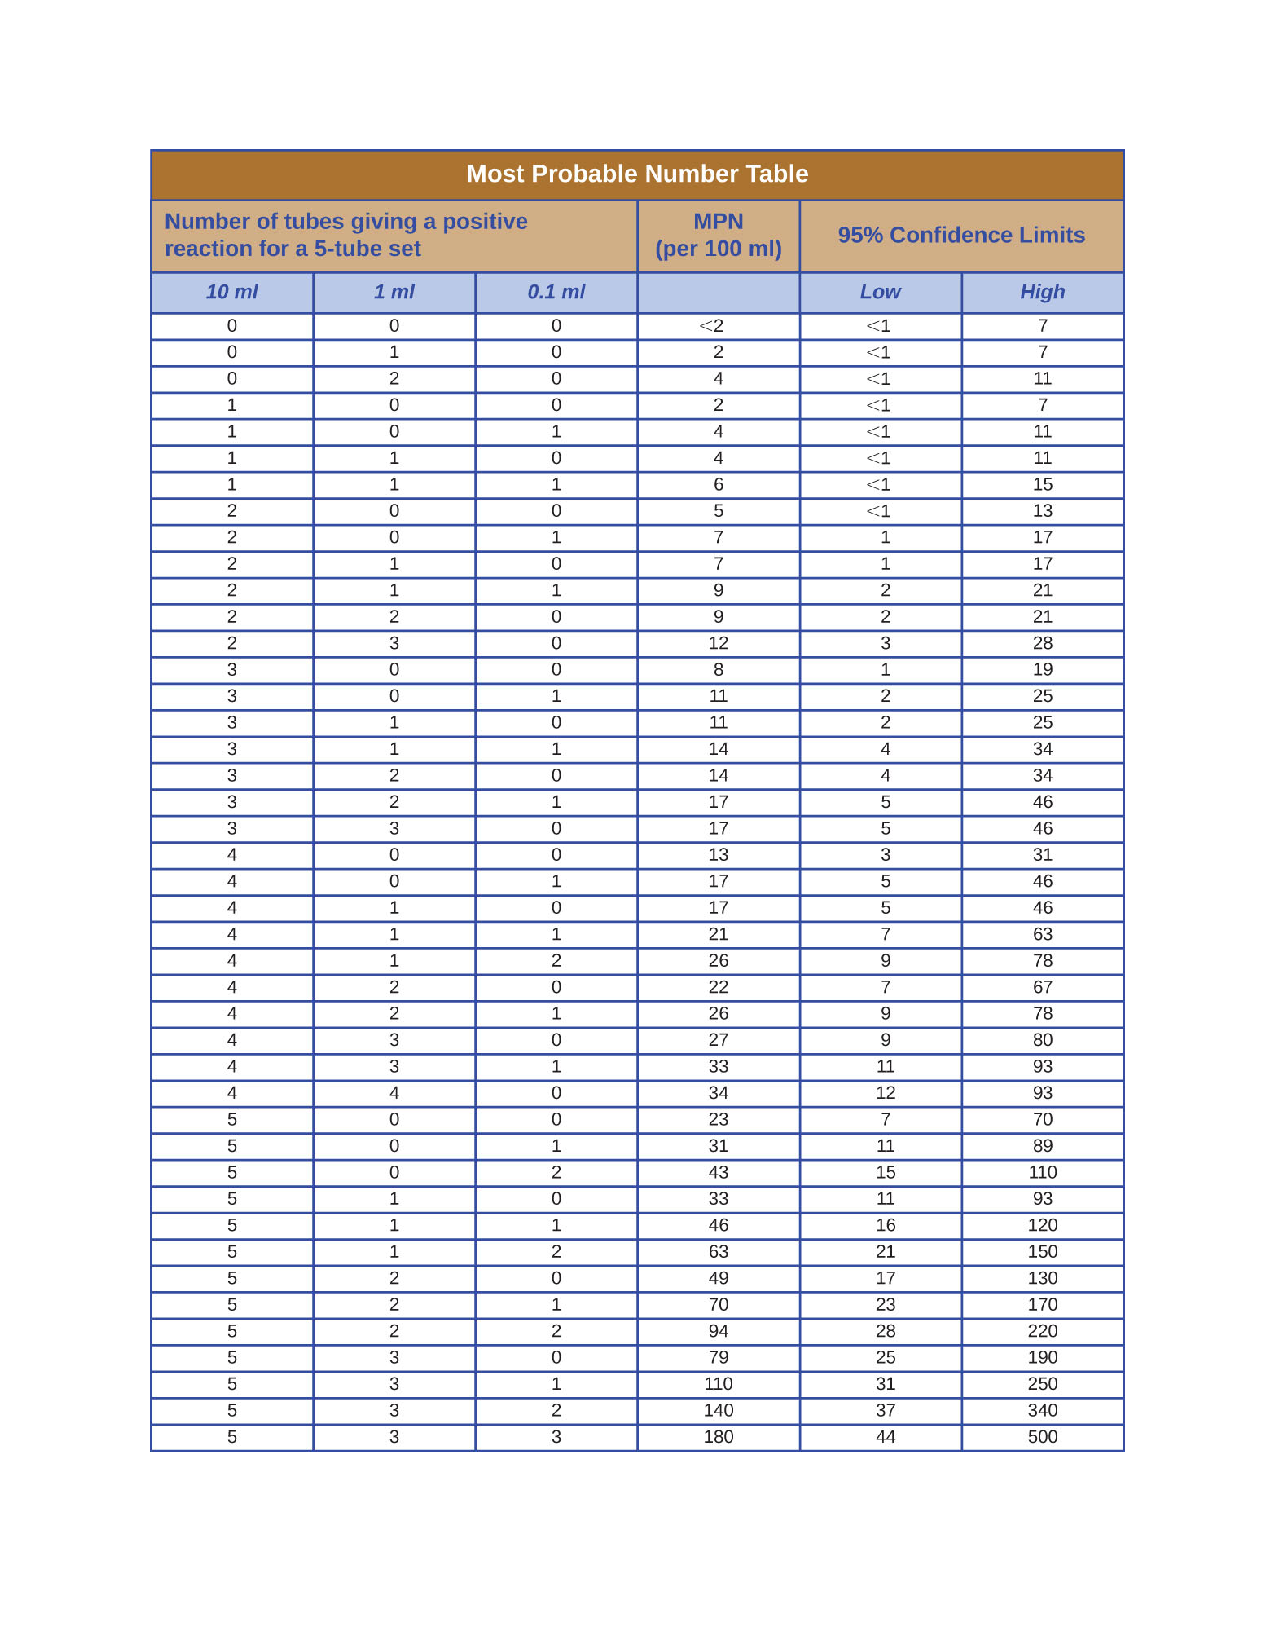
\includepdf[]{MTFTable.pdf}


\newpage

\subsection{Presence - absence (P-A) method}\index{Microbial testing!Presence-absence (P-A) method}
\begin{itemize}
\item Presence - Absence Method below is to assess the presence or absence of bacteria as required by the Revised Total Coliform Rule.
\item The Presence - Absence (P-A) Method for total coliform is based on two premises:
\begin{enumerate}
\item No coliform bacteria should be present in 100 mL of drinking water, and
\item If one viable cell is present it will multiply to give a population of cells that will ferment lactose to produce acid and gas.
\end{enumerate}

\item P-A Method is a simple modification of the multiple tube (MPN) method. P-A broth contains lactose and a pH indicator, which will change from purple to yellow if lactose is fermented and acid is produced. To this P-A broth, the compound \textbf{MUG} has been added. This initially colorless compound can be hydrolyzed by the E. coli to form a compound that fluoresces under long UV light (336 nm). Observing for fluorescence emission using a long-wave (e.g., 365 nm) UV lamp is a sensitive way to confirm the presence of E. coli in water samples.
 
\item The procedure involves addition of 100 ml of sample to 50 ml of sterile P-A broth and then incubating the inoculated broth at 35\degree{C} and inspected after 24 and 48 hours. Upon incubation, a positive result is indicated by the formation of a distinct yellow coloration of the media and/or gas formation which is indicated by foaming of the media upon gentle shaking of the bottle. 

\item Besides the P-A broth, the Colilert test enzymes (used in the above Quanti-Tray test) can be used to test for the Presence-Absence of coliforms.  The colilert enzyme is added to 100 ml water sample in a sterile, non-fluorescing vessel and incubated at 35\degree{C} for 24 h. The results are read at 24 h (before 28 h) and compared against the comparator. If no yellow color, the test is negative, If the sample has a yellow color equal to or greater than the comparator, the presence of total coliforms is confirmed. If yellow, check for blue fluorescence by placing a 6W, 365 nm UV light within 5 inches of the sample. If blue fluorescence is greater or equal to the fluorescence of the comparator the presence of E. coli is confirmed. 
\end{itemize}

\subsection{Heterotrophic plate count (HPC) }\index{Microbial testing!Heterotrophic plate count (HPC)}
\begin{itemize}
\item HPC test - also known as Standard Plate Count is used to measure the overall bacteriological quality of drinking water.
\item  It measures colony formation of heterotrophic bacteria present on culture media. HPC testing indicates the culturable organisms present, which could be as low as 1\% of the total bacteria present. 
\item Heterotrophs are a group of microorganisms including bacteria, molds and yeasts, that use organic carbon sources to grow and can be found in all types of water. Majority of bacteria found in drinking water systems are considered heterotrophs.
\item As all heterotrophic organisms are not pathogens and all pathogens are not heterotrophic, HPC results are not an indicator of water safety.
\item There is no maximum acceptable concentration of HPC in drinking water. However, increases in HPC concentrations above baseline levels are considered undesirable.

\item High HPC counts indicate ideal conditions for bacterial regrowth and should be corrected. Bacterial regrowth can lead to pipe corrosion, encourage slime growth, increase the need for disinfectants, cause foul-tasting water, and harbor secondary respiratory pathogens (ex. Legionella). Thus, HPC can be used as a marker for the underlying causes of some aesthetic problems

\item Methods used for routine testing of heterotrophic bacteria are
\begin{enumerate}
\item Pour plate method: \index{Microbial testing!Heterotrophic plate count (HPC)!Pour plate method}In this method, the liquid sample is poured into the petri dish before the solidification of the agar medium. After solidification, colonies grow both inside and on the surface of the medium.
\item Spread plate method \index{Microbial testing!Heterotrophic plate count (HPC)!Spread plate method}: Here the water sample is spread evenly over the surface of an agar plate medium.  A successful spread plate will have a countable number of isolated bacterial colonies evenly distributed on the plate.
\item Membrane filtration method \index{Microbial testing!Heterotrophic plate count (HPC)!Membrane filtration method}: This test uses a membrane filter is used to capture the bacteria as the water sample is filtered through it.  The filter is placed on an absorbent pad (in a petridish) saturated with a culture medium suitable for heterotrophe growth.
\end{enumerate}

\end{itemize}

\subsection{Other coliform quantification tests}
\ul{Membrane Filtration Method}\index{Microbial testing!Membrane filtration}
Membrane filtration (\textbf{MF}) is a faster way to estimate bacterial populations in water.  In this method, an appropriate sample volume is passed through a membrane filter with a pore size small enough (0.45 micron) to retain the bacteria present. The filter is placed on an absorbent pad (in a petri dish) saturated with a culture medium that is selective for coliform growth. The petri dish containing the filter and pad is incubated, upside down, for 24 hours at the appropriate temperature. After incubation, the colonies that have grown are identified and counted using a low power microscope. A MUG medium is used for E- Coli.  If E. Coli is present, it will make the MUG fluorescent when viewed in UV light. 


\begin{figure}[!htb]
    \centering
       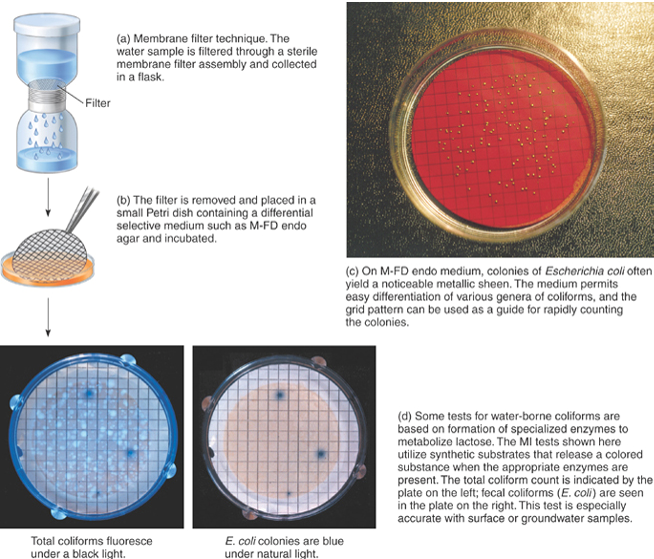
\includegraphics[width=\linewidth]{LaboratoryMembraneFiltration}
        \caption{Multiple tube fermentation}
    \end{figure}
    
\ul{Quanti-trays tests}\index{Microbial testing!Quanti-trays tests}

This test used for the detection and quantification of specific microorganisms is being used increasingly mainly because it is a quicker test than the MTF.  Colilert and Enterolert \index{Microbial testing!Colilert} are the quanti tray based tests for E. Coli and Enterococcus.  This method involve the use of specific enzymes and overcomes the drawbacks of the MTF which include false positives and negatives due to the more generic nature of the media used.
\begin{figure}[!htb]
    \centering
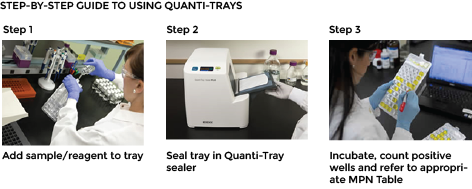
\includegraphics[width=\linewidth]{LaboratoryQuantiTray}
\caption{Quanti-trays test}
\end{figure}

\section{Sampling}\index{Sampling}

		\begin{itemize}
			\item Field or laboratory measurement of a certain parameter is critical in water treatment and distribution operations to obtain information about characteristics of water.
			\item A sample is a small part of the whole representing the whole.  Thus, a sample needs to be such that it truly represents the entire population – which could be either a treatment process stream or what is provided to the end user.
			\item As not all water is analyzed, a sample obtained for analysis must “represent” varying:
			\begin{itemize}
			\item Locations:  Locations should be representative of the majority of their portion of the Distribution System. Unusual locations should be avoided, as they are not indicative of the system as a whole.  Such locations are often monitored, but not as part of the routine plan.

			\item Time periods: Time period samples include:
			\begin{itemize}
			\item Grab: \index{Sampling!Grab} Sample taken in a single moment of time.
			\item Composite: \index{Sampling!Composite} Several portions collected over time and/or space.
			\item Continuous

			\end{itemize}
		\end{itemize}
		\end{itemize}


\subsection{Sampling methods}\index{Sampling!Sampling methods}

\subsubsection{Grab samples}\index{Sampling!Grab samples}
				\begin{itemize}
					\item A grab sample is a sample collected at a specific spot at a site over a short period of time.  
					\item Grab sampling allows for instantaneous analysis of parameters such as pH, dissolved oxygen, chlorine residual, temperature and other parameters which change rapidly with time.
					\item A grab sample represents a snapshot of space and time of a process stream.
					\end{itemize}

\subsubsection{Composite Samples}\index{Sampling!Composite Samples}
				\begin{itemize}
					\item A composite sample is a collection of discrete samples are combined over a certain period or space and therefore represent the average performance of a treatment plant or a process during the collection period.\\  
					\item Composite sampling can be either based on:
					      
					      1. constant time interval (time-proportioned sampling)\index{Sampling!Composite!time-proportioned sampling}\\
					      2. constant volume interval (flow-proportioned sampling), \index{Sampling!Composite!flow-proportioned sampling}and\\
					      3. treatment process space - includes samples taken at different depths \index{Sampling!Composite!depth sampling}\\
					      
					\item Composite samples are typically collected using automated samplers which can be programmed to collect samples at preset time intervals – for time proportional sampling.
					\item Time and space composite samples are collected by adding equal volumes of samples collected from different times or locations.  
					\item Flow proportional composite samples comprise of volume of each subsample based on flow.\\  
				\end{itemize}
	\begin{figure}			
			\begin{center}
				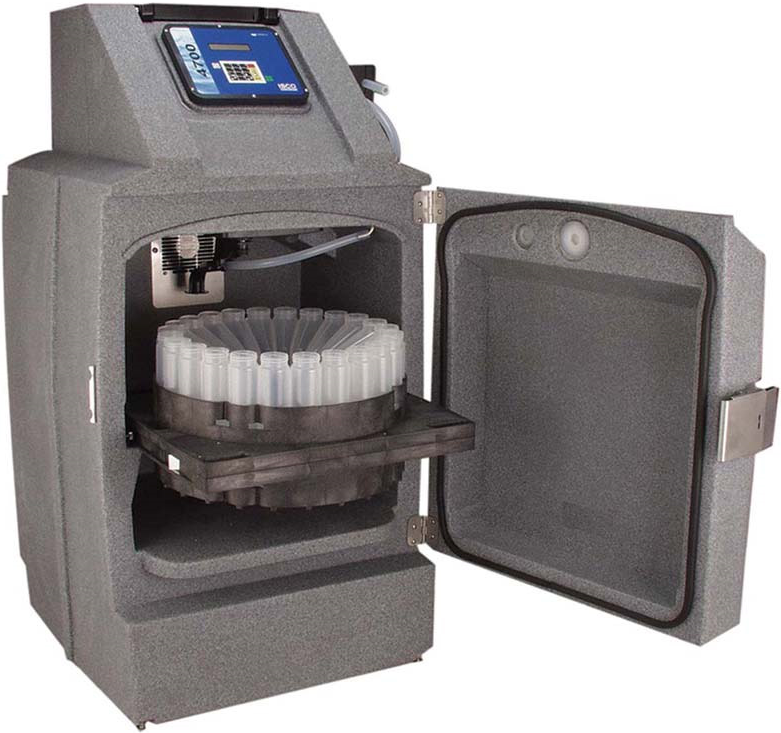
\includegraphics[scale=0.2]{Autosampler} \hspace{2cm} 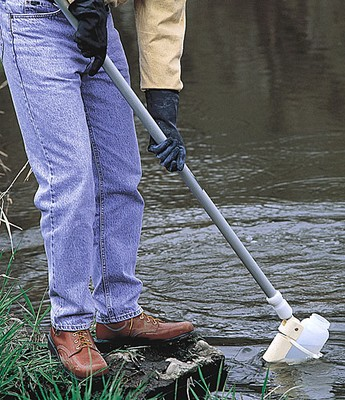
\includegraphics[scale=0.37]{Grabsampler}\\
			\end{center}
			\hspace{2.3cm} Automated Sampler \hspace{2.0cm} \parbox{\textwidth}{Grab Sampling Using a Long Handle Dipper}\\
\end{figure}
\subsection{Sampling precautions and protocols}\index{Sampling!Precautions and protocols}
			\begin{itemize}
				\item Samples should represent the major portion of the process or the process stream and should be taken from places where the mixing is thorough, avoiding dead spots and areas of heavier or lighter loadings. 
				\item The collected sample is invariably exposed to conditions very different from the original source and is subject to change due to chemical and microbiological activity.  
				\item Thus, in order to ensure integrity of sample, sample preservation techniques specific to the analysis to be performed is needed.  
				      \begin{itemize}
				      	\item The preservation technique should not only allow for stabilizing the parameter to be analyzed, it should also not interfere with the analyses.  
				      	\item The common preservation techniques involve use of proper containers, temperature control, addition of chemical preservatives, and observance of the recommended maximum sample holding time.
				      \end{itemize}
				      \item Samples cannot be held indefinitely prior to lab analysis
\item  Laboratories used for testing must be approved by Environmental Laboratory Accreditation Program {ELAP} \index{Environmental Laboratory Accreditation Program (ELAP)} and must use Standard Methods.
\item Chain-of-custody \index{Chain-of-custody}ensures sample integrity from collection to data reporting Important for sample control when litigation is involved Must be under a person’s physical possession, within sight, or secured in a restricted area Receipt and logging of sample at lab Complete documentation from collection to report
\item Sample Containers:
\begin{itemize}
\item Typically plastic or glass
\item Use proper material for analysis
\item Use glass for all organic and odor analyses
\item Use plastic for metals
\item Bacteriological sample containers must be sterile
\end{itemize}
\end{itemize}

\subsection{Microbial sampling}\index{Sampling!Microbial sampling}
\begin{itemize}
\item Always collected as a grab.
\item The sample is obtained from a steady, pencil-width stream from a cold water fixture, only after it has been in a wide open setting and  water to run a minimum of five minutes to flush out the bacteria from the surface. 
\item A clean, sterile borosilicate glass or plastic bottle containing sodium thiosulfate is used. Sodium thiosulfate is added to remove residual chlorine which will kill the microorganisms during transit. If the sample is not preserved or maintained under proper conditions until the test is conducted in the laboratory, the test would provide erroneous results
\item Samples must be refrigerated if they cannot be analyzed within 1 hour of collection
\item Samples must be handled with care to prevent contamination and adverse conditions such as prolonged exposure to direct sunlight
\item Maximum holding time for state or federal permit reporting purposes is 6 hours
\item Number of samples collected depends on number of customers served/and is according to the approved sample siting plan.
\item The volume for coliform compliance sample must be at least 100ml and no more than 120ml. 
\item Sealed and sterilized sampling bottles - typically, 120 ml with 100 ml marked to provide space for air is used.
\item Sodium thiosulfate or some other de-chlorinator \index{Chlorine disinfection!Dechlorination}is pre-added to the sampling bottle. A dechlorinator is critical to ensure any chlorine residual is removed from the sample collected.
\item The faucet is opened to obtain a continuous flow of the size of a pencil, the faucet should not be opened under a strong flow as  that could potentially dislodge loose particles/slime growth in the mains.
\item When the cap is opened to collect the sample, care needs to be taken to ensure the cap is not contaminated.
\item Fill the bottle to the marked fill-line leaving an air gap - do not overfill.
\item The capped bottle should be placed in an iced container and transported to the laboratory as soon as possible.
\item Follow chain-of-custody \index{Chain-of-custody}and send the bottles to the lab with paperwork.
\item In the laboratory, the samples must be kept at 4\degree{C} or 39\degree{F} and must be analyzed preferably within 8 hours and never to exceeding 24 hours.
\item The analytical results shall be reported in terms of the presence or absence of total coliforms and E. coli, in the sample, whichever is appropriate.
\item Monthly sampling results must be submitted to the regulatory agency per established scheduled.
\item Records of bacteriological sampling must be kept for five years \index{Bacteriological sampling records}.
\item Repeat sampling:  If the result is positive a minimum three samples need to be taken, one from the original point, one up-stream and one from downstream of the original sample collection site within 24 hours after the result notification from the laboratory.
\item False positive means that the sample when tested is found to be contaminated but
actually the water is safe.
\item False negative means samples are found to be safe; even though the water is
- unsafe to drink. This can lead to outbreak of diseases and cause customers to lose confidence in their drinking water supplier. This harms the customer. \index{False negative/positive}
\end{itemize}
\newpage
\subsection{Summary of sampling requirements}\index{Sampling!Summary of sampling requirements}\index{Sampling!Preservative}\index{Sampling!Holding time}
\begin{table}[h!]
\begin{tabular}{|p{4cm}|p{3cm}|p{4cm}|p{3cm}|}
\hline
\multicolumn{1}{|c|}{\textbf{Parameter}}                                                   & \multicolumn{1}{c|}{\textbf{Container}}                                            & \multicolumn{1}{c|}{\textbf{Preservative}}                                                                                                                   & \multicolumn{1}{c|}{\textbf{Holding Time}}                          \\ \hline
\begin{tabular}[c]{@{}l@{}}Coliform, total or fecal,\\      in chlorinated water\end{tabular} & \begin{tabular}[c]{@{}l@{}}Sterile container    w/\\      thiosulfate\end{tabular} & Cool   to \textless{}10 °C.  Do not freeze                                                                                                                    & 8   hrs for source water compliance and 30 hours for drinking water \\ \hline
Giardia and   Cryptosporidium                                                              & 10   L plastic container                                                           & Cool   to \textless{}10  °C .  Do not freeze                                                                                                                    & 96   hours                                                          \\ \hline
Alkalinity, turbidity, solids                                                             , fluoride & Plastic or Glass                                                                   & Cool   to \textless{} 4 °C                                                                                                                                             & Method   dependent                                                  \\ \hline
Metals, general                                                                            & Plastic or Glass, Rinsed w/ 1:1 HNO$_3$                                               & Nitric   acid to pH \textless 2                                                                                                                              & 6 Months                                                            \\ \hline
Hardness                                                                           & Plastic or Glass                                                                   & Nitric   acid to pH \textless 2                                                                                                                              & 6 Months                                                            \\ \hline
pH                                                                                         & Plastic or Glass                                                                   & None                                                                                                                                                         & Analyze in 15 min                                                    \\ \hline
Nitrogen and   phosphorous compounds                                                       & Plastic or Glass                                                                   & Sulfuric acid to   pH\textless{}2                                                                                                                            & 28 days                                                             \\ \hline
VOCs, TTHMs                                                                                & Glass bottle                                                                       & Sodium thiosulfate or   ascorbic acid if sample is chlorinated and hydrochloric acid (HCl) to pH \textless 2  and cool to  \textless 4 °C  but do not freeze & 14 days                                                             \\ \hline
\end{tabular}
\caption{Summary of sampling requirements for key parameters}\index{Sampling!Summary of requirements}
\end{table}






\part{Module 3}
\input{Math1.tex}
\part{Module 4}
\chapterimage{Water1}
\chapter{Water Properties and Sources}





\begin{table}[H]
\begin{tabular}{| m{1cm} | m{15cm} |}
\hline
\multicolumn{2}{|l|}{\textbf{Expected   Range of Knowledge for Water Properties and Sources}}                                                                          \\ \hline
\multicolumn{2}{|l|}{\textit{Water   Distribution System Operator License Exams}}                                                                                      \\ \hline
D1 & Ability to measure   well depth                                                                                                   \\ \hline
D1 & Ability to recognize   potential sources of contamination                                                                         \\ \hline
D1 & Knowledge of the   hydrologic cycle                                                                                               \\ \hline
D1 & Knowledge of security   procedures/measures                                                                                       \\ \hline
D1 & Ability to calculate   draw down                                                                                                  \\ \hline
D1 & Ability to recognize   abnormal pH levels of water in a distribution system                                                       \\ \hline
D1 & Ability to recognize   abnormal turbidity levels in a distribution system                                                         \\ \hline
D1 & Knowledge of normal   pH range in drinking water                                                                                  \\ \hline
D1 & Knowledge of the   impacts of high nitrate concentrations in a distribution system                                                \\ \hline
D1 & Knowledge of the   meaning of high levels of turbidity in a distribution system                                                   \\ \hline
D1 & Knowledge of   contamination sources in a well                                                                                    \\ \hline
D1 & Knowledge of water   storage contamination sources                                                                                \\ \hline
D1 & Ability to measure   the water depth in a well                                                                                    \\ \hline
D1 & Knowledge of water   depth measurement techniques                                                                                 \\ \hline
D2 & Knowledge of cone of   depression                                                                                                 \\ \hline
D2 & Knowledge of recovery   time                                                                                                      \\ \hline
D2 & Knowledge of static   and pumping water level                                                                                     \\ \hline
D2 & Knowledge of water   table fluctuations                                                                                           \\ \hline
D2 & Knowledge of well   components and terms                                                                                          \\ \hline
D2 & Knowledge of well   protection                                                                                                    \\ \hline
D2 & Knowledge of zone of   influence                                                                                                  \\ \hline
D2 & Knowledge of proper   installation of a sanitary seal on a well                                                                   \\ \hline
D3 & Knowledge of the   vulnerability assessment                                                                                       \\ \hline
D3 & Knowledge of well   location requirements                                                                                         \\ \hline
D3 & Knowledge of the   chemical components of groundwater                                                                             \\ \hline
D3 & Ability to calculate   specific yield                                                                                             \\ \hline
\end{tabular}
\end{table}

\newpage



\begin{table}[H]
\begin{tabular}{| m{1cm} |m{15cm} |}
\hline
\multicolumn{2}{|l|}{\textbf{Expected   Range of Knowledge for Water Properties and Sources}}                                                                      \\ \hline
\multicolumn{2}{|l|}{\textit{Water   Distribution System Operator License Exams (Continued)}}                                                                  \\ \hline
D4 & Knowledge of long-term water availability                                                                                         \\ \hline
D4 & Knowledge of sanitary survey requirements                                                                                         \\ \hline
D4 & Knowledge of the characteristics of   aquifers                                                                                    \\ \hline
D4 & Knowledge of proper gravel packing and   screen depth                                                                             \\ \hline
D4 & Knowledge of well abandonment procedures and   permit requirements                                                                \\ \hline
D4 & Ability to estimate future water needs                                                                                            \\ \hline
D4 & Knowledge of capital improvement/capital   replacement requirements                                                               \\ \hline
D5 & Knowledge of permit   requirements                                                                                                \\ \hline
\multicolumn{2}{|l|}{\textit{Water   Treatment System Operator License Exams}}                                                                  \\ \hline
T1 & Ability to recognize   abnormal well operations                                                                                   \\ \hline
T1 & Ability to recognize   potential security risks                                                                                   \\ \hline
T1 & Ability to recognize   potential sources of contamination in surface water                                                        \\ \hline
T1 & Ability to recognize   the influence of surface water on a groundwater source                                                     \\ \hline
T1 & Knowledge of flow   measurement devices                                                                                           \\ \hline
T1 & Knowledge of   potential microbial and chemical contamination sources in groundwater and   surface water                          \\ \hline
T1 & Knowledge of the   characteristics of aquifers                                                                                    \\ \hline
T1 & Knowledge of the   hydrologic cycle                                                                                               \\ \hline
T1 & Knowledge of visual   signs of contamination in a surface water reservoir                                                         \\ \hline
T1 & Knowledge of well   components                                                                                                    \\ \hline
T1 & Knowledge of well   depth measurement procedures                                                                                  \\ \hline
T1 & Knowledge of well   disinfection procedures                                                                                       \\ \hline
T1 & Knowledge of well   drawdown measurement techniques                                                                               \\ \hline
T1 & Knowledge of   waterborne pathogens                                                                                               \\ \hline
T1 & Ability to interpret   water quality reports                                                                                      \\ \hline
T2 & Ability to   discriminate between normal and abnormal conditions of a surface water   reservoir                                   \\ \hline
T2 & Ability to recognize   hydrological changes                                                                                       \\ \hline
T2 & Knowledge of how   reservoir intake level effects water quality                                                                   \\ \hline
T2 & Knowledge of the   effects of seasonal changes on water reservoirs                                                                \\ \hline
T3 & Knowledge of surface   water reservoir stratification                                                                             \\ \hline
T3 & Ability to recognize   head loss across an intake screen                                                                          \\ \hline
T3 & Knowledge of   groundwater treatment procedures                                                                                   \\ \hline

T4 & Ability to interpret historical water use data                                                                                   \\ \hline
\end{tabular}
\end{table}

\newpage







































\section{Properties of water}\index{Properties of water}
\begin{itemize}
\item Water is one of the most abundant and common materials on earth. It covers 70 percent of the surface of the earth as water and ice.
\item Water makes up 60-75\% of human body weight. A loss of just 4\% of total body water leads to dehydration, and a loss of 15\% can be fatal.
\item A person could survive a month without food but would not survive 3 days without water \index{Human body component}.
\item Even though most other planets have water in some form, the earth is the only planet in the solar system that contains water in all its common forms (gas, liquid, solid).  Others have ice, but only the earth has an abundance of this miraculous substance in the proper temperature range to support life.
\item Its chemical formula, H$_2$O, indicates that each of its molecules contains one oxygen and two hydrogen atoms.  
\item The much larger oxygen atom is connected by covalent bonds to each of the two hydrogen atome. The hydrogen atoms are attached to the oxygen atom at an angle of 104.45\si{\degree}.
\item Even though the water molecule is overall neutral, its bent shape results in the accumulation of positive charge near the oxygen end and negative charge near the hydrogen.  This differential in charges makes the water molecule \textbf{polar} \index{Polar} - like a magnet and bestows it unique properties. 
\item The polarity and molecule size of water imparts it a unique property of being able to dissolve a very wide range of minerals, chemicals and gases which makes it indispensable for the existence of lifeforms and a very critical element of our day-to-day life.  However, many of the substances dissolved in water must be removed during treatment to make water safe to drink.
\item Nonpolar substances such as oils, fats, and many organic compounds do not dissolve as easily in water.
\begin{figure}[h]
\begin{center}
        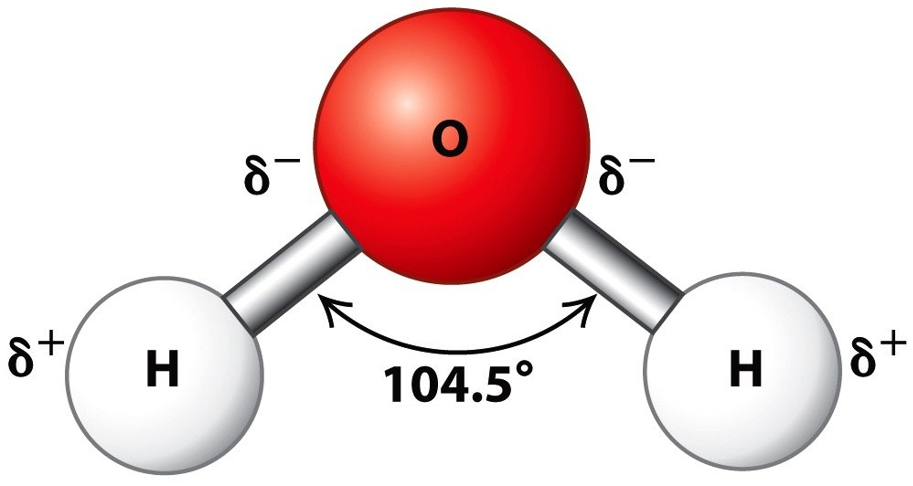
\includegraphics[scale=0.25]{WaterMolecule}
        \caption{Water molecule}
        \label{Water molecule}
\end{center}
\end{figure}
\vspace{0.5cm}

\item Pure water will not conduct electrical current. But when soluble salts such as sodium chloride (NaCl), calcium carbonate (CaCO$_3$) are present in water, water will conduct electricity as these salts ionize - break into its constituent positive and negative charged particles the water, and the charged ions make water to conduct electrical current.
$$NaCl \leftrightarrow Na^+ + Cl^-$$
\item The more ions there are in a solution, the more easily the current flows. The ability to conduct electrical current is called conductivity and can be used to indirectly estimate the amount of total dissolved solids in the water.\\
\item The boiling of water - 100\si{\degree}C or 212\si{\degree}F and its melting/freezing point - 0\si{\degree}C or 32\si{\degree}F is very high  compared to similar molecules and it is the only natural substance found in all three physical states at the temperatures that naturally occur on Earth.
\item Most other substances become more dense as they cool.  However, ice is less dense than water which makes ice float on water.
\item Ice on the water surface insulates the water below preventing it from freezing and allowing for fish and other life form to survive and allows for the movement of animals who live in these cold habitats.
\item As water cools, its density increases upto 4\si{\degree}C after which it gets less dense as it is cooled further.
\item The changing density of water is responsible for turnover of a lake during fall.  When the surface water cools, the cold water becomes more dense than the warm water below so the cold water sinks to the bottom and warm water rises to the top.  When lakes are used as the source water for water treatment plants, turnover can cause abrupt changes in the quality of raw water.
\item It needs a lot of energy to make the water warmer or cooler (high Specific Heat) which allows for keeping the temperature of water bodies such as oceans, rivers, ponds more or less constant despite the heat from the sun.
\item Water molecules stick together well because of its high surface tension - which allows for water to rise up in tubes through capillary action.  This capillary action allows for plants to draw water along with nutrients from the ground.
\end{itemize}


\section{Water use}\index{Water use}
\begin{itemize}
\item Besides it being needed for basic sustenance of all living beings, water is vital element for the world economy and sustenance of the human society in various ways including:
\begin{itemize}
\item As a food source - fishing
\item For commerce - shipping, trade and transportation
\item For recreation - swimming, skiing, surfing etc.
\end{itemize}
\item Breakdown of global freshwater use:\\
70\% is used for agriculture\\
19\% is used by industries, and \\
11\% is for municipal use
\end{itemize}

\section{Water supplies}\index{Water supplies}
\begin{itemize}
\item Civilizations have always formed near water sources - on the banks of rivers. Ancient Egyptians - on the Nile, Mesopotamians in the Fertile Crescent on the Tigris/Euphrates rivers, Ancient Chinese on the Yellow River, and the Ancient India on the Indus.
\item The water on our Earth today is the same water that has been here for nearly 5 billion years.\\
\item Water molecules were formed in interstellar space by chemical reactions between hydrogen molecules and oxygen-bearing molecules such as carbon monoxide and the Earth inherited its water from asteroids and comets crashing into it.
\item The only thing that changes is the form that water takes as it travels through the water cycle.
\item On Earth, water is the only substance that can occur naturally in its three states of matter -  gas, liquid and solids, circulates naturally through its five principal realms:
\begin{itemize}
\item Oceans
\item Atmosphere
\item Lakes and rivers
\item Icecaps and glaciers
\item Underground
\end{itemize}
This is the planetary Water Cycle. \index{Water cycle}
\item Elements of the water cycle include:
\begin{itemize}
\item Transpiration - process by which plants lose water as vapor out of their leaves. 
\item Evaporation - conversion of water in oceans, rives and lakes into vapor by the heat from the sun
\item Evapotranspiration is the combined processes of evaporation and transpiration - the movement of water from oceans or land to the atmosphere.
\item Condensation - cooling of water vapor in the upper layer of earths atmosphere into liquid water in the form of clouds
\item Precipitation - discharge of the water bearing clouds as rain, hail, sleet or snow.
\item Infiltration - movement of water from surface to soil.
\end{itemize} 
\item Life on earth is dependent on the Earth's water cycle \index{Water cycle}
\begin{figure}[]
\begin{center}
\includegraphics[scale=0.8]{Watercycle1}\index{Water cycle}
\caption{Water cycle}
\label{Water cycle}
\textit{(Credit:David Cain/NWS)}
\end{center}
\end{figure}
\item A watershed \index{Watershed} is the area of land, where all of the water that falls in it and drains off of it into to a common outlet which could be a one or combination of water bodies such as a river, lake or underlying groundwater.
\item The natural features including - mountains, trees, shrubs, grasses, and man-made features such as urban area, industries, wastes and water discharges affect the quality of the water in or from the watershed.
\item Watersheds are important sources of drinking water, as well as a habitat for many aquatic species. Healthy watersheds with intact native vegetation and wetlands provide important functions such as water purification, flood control, nutrient recycling, and groundwater recharge.
\item Water covers about 71\% of Earth's surface.  The distribution of Earth's water \index{Distribution of earth's water} is provided in the below table.

% Please add the following required packages to your document preamble:
% \usepackage{multirow}
\begin{table}[ht]
\begin{center}
\begin{tabular}{|l|l|llll}
\hline
\multirow{9}{*}{Fresh water} & \multirow{9}{*}{2.50\%} & \multicolumn{1}{l|}{\multirow{7}{*}{Surface water}} & \multicolumn{1}{l|}{\multirow{7}{*}{1.20\%}} & \multicolumn{1}{l|}{Atmosphere}                & \multicolumn{1}{l|}{3.00\%}  \\ \cline{5-6} 
                             &                         & \multicolumn{1}{l|}{}                               & \multicolumn{1}{l|}{}                        & \multicolumn{1}{l|}{Living things}             & \multicolumn{1}{l|}{0.26\%}  \\ \cline{5-6} 
                             &                         & \multicolumn{1}{l|}{}                               & \multicolumn{1}{l|}{}                        & \multicolumn{1}{l|}{Rivers}                    & \multicolumn{1}{l|}{0.49\%}  \\ \cline{5-6} 
                             &                         & \multicolumn{1}{l|}{}                               & \multicolumn{1}{l|}{}                        & \multicolumn{1}{l|}{Swamps, marshes}           & \multicolumn{1}{l|}{2.60\%}  \\ \cline{5-6} 
                             &                         & \multicolumn{1}{l|}{}                               & \multicolumn{1}{l|}{}                        & \multicolumn{1}{l|}{Soil moisture}             & \multicolumn{1}{l|}{3.80\%}  \\ \cline{5-6} 
                             &                         & \multicolumn{1}{l|}{}                               & \multicolumn{1}{l|}{}                        & \multicolumn{1}{l|}{Lakes}                     & \multicolumn{1}{l|}{20.90\%} \\ \cline{5-6} 
                             &                         & \multicolumn{1}{l|}{}                               & \multicolumn{1}{l|}{}                        & \multicolumn{1}{l|}{Ground ice and permafrost} & \multicolumn{1}{l|}{69.00\%} \\ \cline{3-6} 
                             &                         & \multicolumn{1}{l|}{groundwater}                   & \multicolumn{1}{l|}{30.10\%}                 &                                                &                              \\ \cline{3-4}
                             &                         & \multicolumn{1}{l|}{Glaciers and ice caps}          & \multicolumn{1}{l|}{68.70\%}                 &                                                &                              \\ \cline{1-4}
Other saline   water         & 0.90\%                  &                                                     &                                              &                                                &                              \\ \cline{1-2}
Oceans                       & 96.50\%                 &                                                     &                                              &                                                &                              \\ \cline{1-2}
\end{tabular}
\caption{Distribution of earth's water} \index{Earth's water} \label{Earth's water}
\textit{(From:  Igor Shiklomanov's chapter "Worlds fresh water resources" in Peter H. Gleick (editor), \\1993, Water in Crisis: A guide to the world's Fresh water resources)}
\end{center}
\end{table}

\begin{figure}[]
\begin{center}
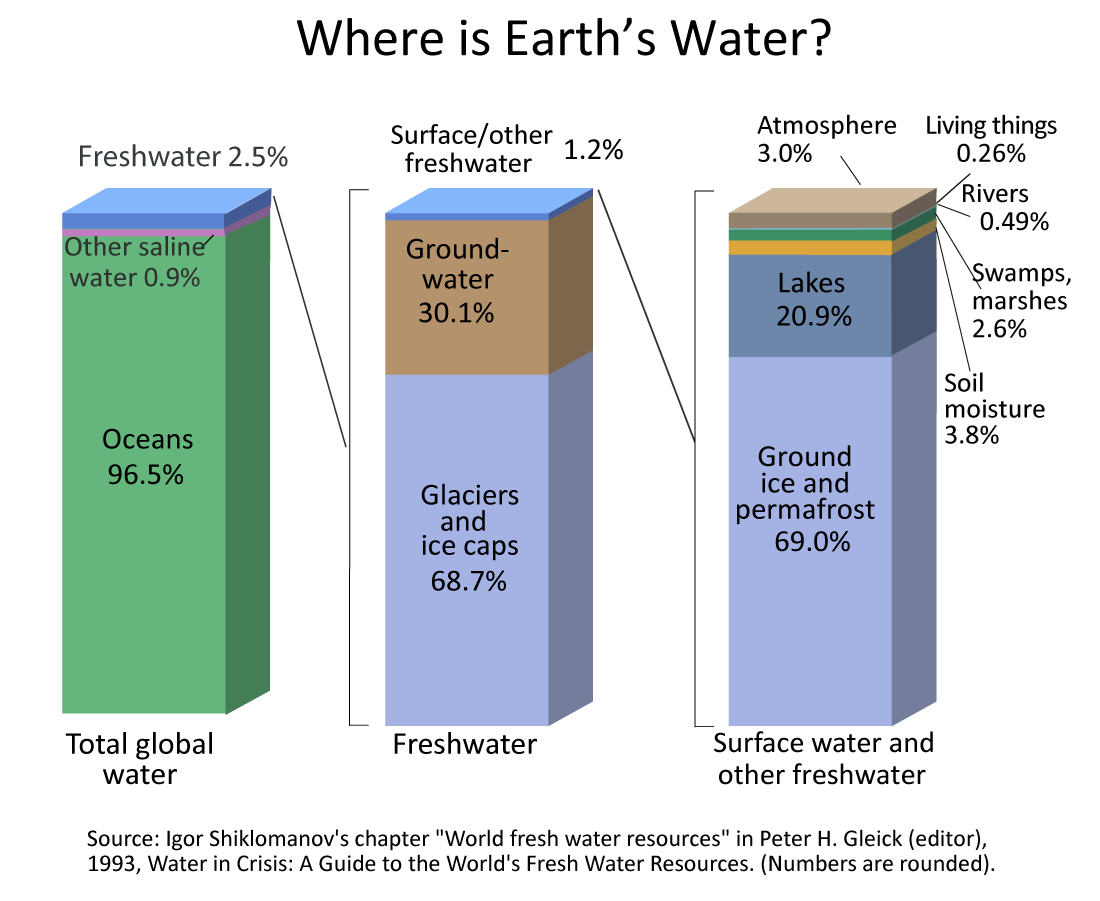
\includegraphics[scale=0.5]{EarthsWater}
\caption{Distribution of earth's water} \index{Distribution of earth's water} \label{Distribution of earth's water}
\textit{(From:  Igor Shiklomanov's chapter "Worlds fresh water resources" in Peter H. Gleick (editor), \\1993, Water in Crisis: A guide to the world's Fresh water resources)}
\end{center}
\end{figure}

\item 97\% of the Earth's water can be found in our ocean and freshwater is only 2.5\% of all the water on earth
\item Most of the fresh water is in form of ice in glaciers, ice caps and permafrost.  
\item A very very small fraction - about 0.006\% of the total water is the freshwater in lakes and rivers.  Most of the remaining freshwater is in groundwater - about 0.75\% of the total water or about 30\% of the total freshwater.
\item Clean water is vital to our health, communities, and economy. 
\item There is no universally accepted definition of “safe drinking water.” Generally speaking, safe drinking water, is defined as the water that does not represent any significant risk to health over a lifetime of consumption.
\item Water scarcity can be caused by a mix of hydrological, infrastructural, political and social issues. 
\item In developing countries, water supply and sanitation related factors cause more than 20 percent of deaths of people under age 14. Nearly
half of all people in developing countries have infections or diseases associated with inadequate water supply and sanitation.
\item Chemical contaminants in drinking water arise including arsenic, fluoride or nitrate, emerging contaminants such as pharmaceuticals, pesticides, per- and polyfluoroalkyl substances (PFASs) and microplastics generate public concern.
\item Microbiologically contaminated drinking water can transmit diseases such as diarrhoea, cholera, dysentery, typhoid and polio and is estimated to cause 485 000 diarrhoeal deaths each year.
\item The amount of water that is available for sustenance including agriculture, sanitation and hygiene is limited in many areas of the world.  Billions of people throughout the world are battling daily against enormous difficulties accessing the most basic services.\\
\item Some 1.1 billion people worldwide lack access to water, and a total of 2.7 billion find water scarce for at least one month of the year.
\item Inadequate sanitation is also a problem for 2.4 billion people.  They are exposed to diseases, such as cholera and typhoid fever, and other water-borne illnesses. Two million people, mostly children, die each year from diarrheal diseases alone.\\
\item Many of the water systems that keep ecosystems thriving and feed a growing human population have become stressed. Rivers, lakes and aquifers are drying up or becoming too polluted to use. More than half the world’s wetlands have disappeared.
\item Climate change is altering patterns of weather and water around the world, causing shortages and droughts in some areas and floods in others, changing large-scale hydrological cycle.\\
\item Historical rates of progress would need to double for the world to achieve universal coverage with basic drinking water services by 2030. 
\item To achieve universal safely managed services, rates would need to quadruple. Climate change, increasing water scarcity, population growth, demographic changes and urbanization already pose challenges for water supply systems. 
\item Re-use of wastewater to recover water, nutrients or energy is becoming an important strategy. 
\item Increasingly countries are using wastewater for irrigation; in developing countries this represents 7\% of irrigated land. While this practice if done inappropriately poses health risks, safe management of wastewater can yield multiple benefits, including increased food production.
\end{itemize}


\section{Water sources}\index{Water sources}
\begin{itemize}
\item Source waters refers to the sources of water - the water bodies or means, which provide water needed for domestic, agricultural and industrial uses.
\begin{figure}[h]
\begin{center}
\includegraphics[scale=0.53]{WaterSources}\\
\captionof{figure}{Water supply sources}%\caption{}
\label{Water supply sources}
\end{center}
\end{figure}
\item Water sources include:
\begin{enumerate}
\item Surface water (for example, a lake, river, or reservoir)
\item Groundwater (for example, an aquifer)
\item Recycled water - also called reused water\\
\end{enumerate}
\end{itemize}
\begin{figure}[h!]
\begin{center}
\includegraphics[scale=0.3]{WaterSupplyIllustration1}\\
\captionof{figure}{Illustration of Southern California water supply systems} \label{Illustration of Southern California water supply systems}
\end{center}
\end{figure}

\begin{figure}[h!]
\begin{center}
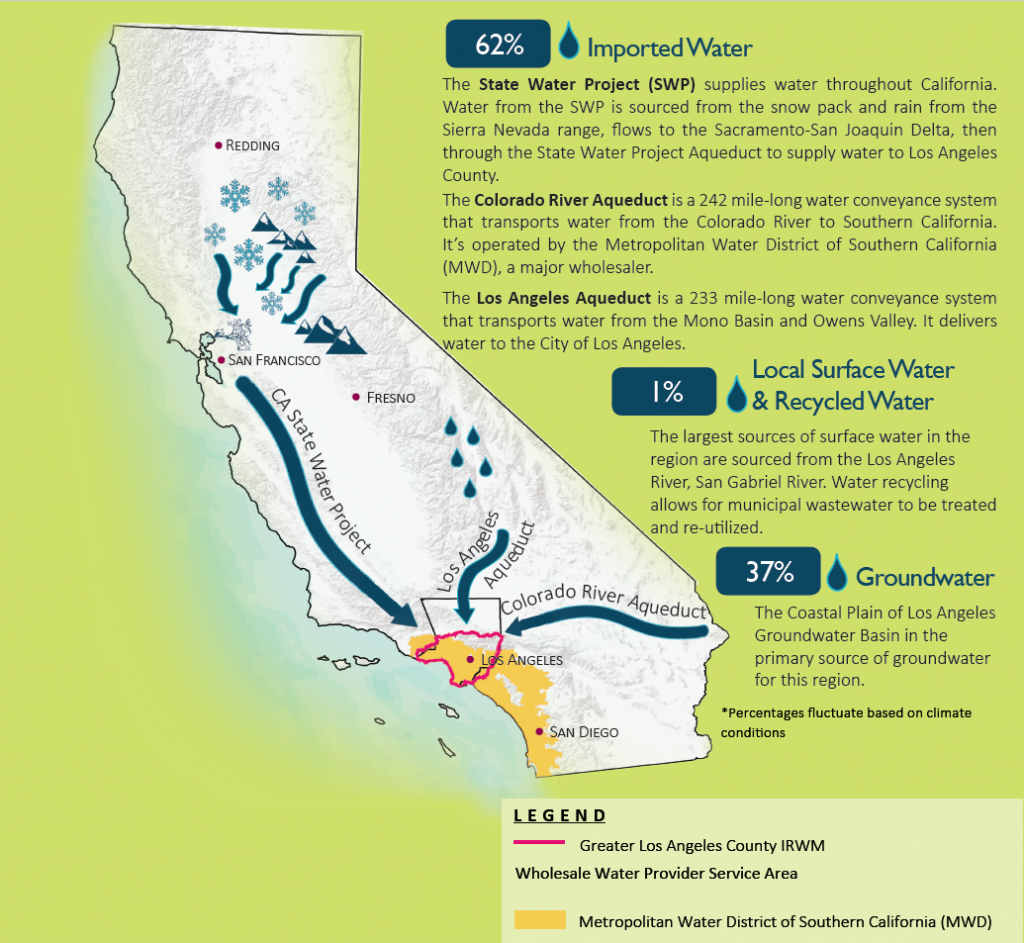
\includegraphics[scale=0.4]{LosAngelesWaterSupply}\\
\captionof{figure}{Los Angeles area source water summary}%\caption{}
\label{Los Angeles area source water summary}
\end{center}
\end{figure}
\subsection{Groundwater}\index{Groundwater}
\begin{itemize}
\item Groundwater is the water found underground in spaces between sand, rock and soil. 
\item Groundwater is stored in aquifers - water-bearing formations underneath the surface that readily transmit water. 
\item \textbf{Aquifers} \index{Aquifer} are underground layers of very porous water-bearing soil or sand with enough groundwater that it can be pumped to the surface and used for drinking water, irrigation, industry, or other uses.
\item Water from precipitation, such as rain or snow, naturally filters through the soil, and is held within the aquifer. 
\item Groundwater can move through the aquifer and resurface through springs and wells.  The rate at which groundwater moves through an aquifer varies depending on the permeability of the layer.
\item Groundwater is extracted from aquifers via well pumping.
\item Groundwater moves from higher elevations to lower elevations and from areas of higher pressure to areas of lower pressure.
\item Groundwater is not stored in huge underground caverns, groundwater fills the pores of the various kinds of rocks that form the earth below us. \textbf{Hydrogeology} is the study of groundwater.
\item The presence of the groundwater depends largely on the geology of a specific area and the variable porosity of the upper portion of the earth’s crust. 

\item Access to groundwater is through:
\begin{enumerate}
\item \textbf{Wells} \index{Wells} - an ordinary well is essentially an a hole in the ground to access the water in the aquifer.
\item \textbf{Artesian Well} - as the groundwater moves in a aquifer, in certain areas of poor permeability, the water is pressurized.  In a well dug in this area, the water level will rise above the top of the aquifer and may even flow onto the land surface - {\textbf{flowing artesian well}}
\item \textbf{Springs} \index{Springs} - which is the flow of groundwater onto the earth's surface through a natural opening.  Springs occur when the contact between an upper aquifer and a lower aquitard intersects the ground surface
\begin{figure}[h]
\begin{tabular}{  m {8 cm}  m {8 cm} } 
\begin{center} \includegraphics[scale=0.6]{GroundWaterSpring} \end{center} & \begin{center}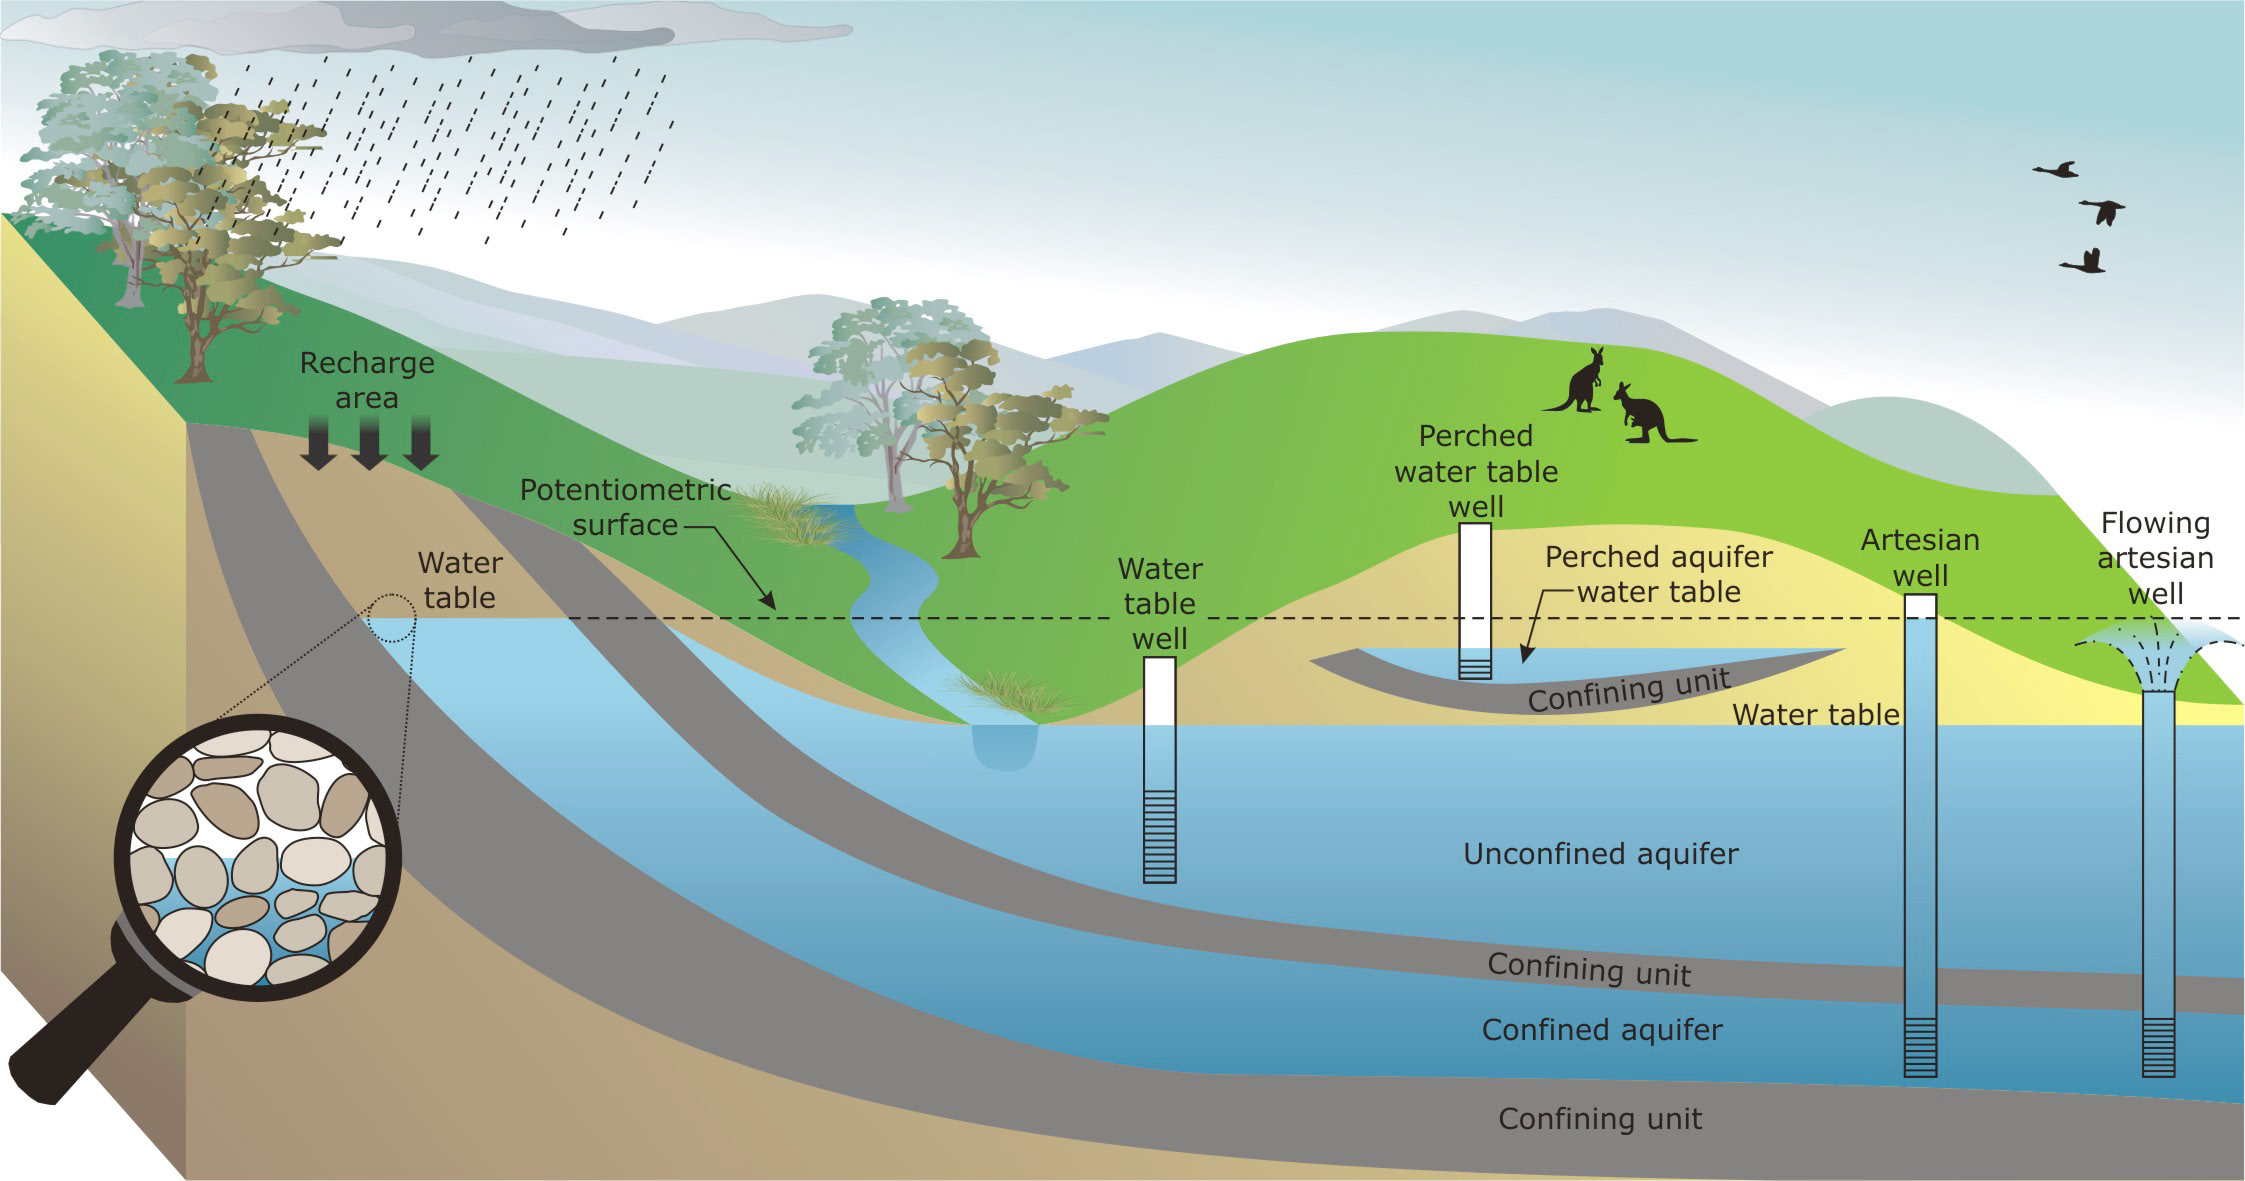
\includegraphics[scale=0.4]{Groundwater1} \end{center}\\
\begin{center} \textbf{Springs} \end{center} & \begin{center}\textbf{Groundwater} \end{center}\\
\end{tabular}\\
\end{figure}
\end{enumerate}
\item There are two general types of aquifers: confined and unconfined. \textbf{Confined Aquifers} \index{Aquifer!Confined and unconfined}have a layer of impenetrable rock or clay above them, while \textbf{Unconfined Aquifers} lie below a permeable layer of soil.
\item The layers of earth which hold the groundwater include a spectrum of layer with porous layer through which the groundwater could through easily in the downward direction, at one end of that spectrum to an \textbf{Aquiclude} which is a geological material through which zero flow occurs.
Then there is the \textbf{Aquitard} \index{Aquifer!Aquiclude, aquitard} in the middle, which is compacted layers of clay, silt or rock that retards the water flow.
\item The replenishment of aquifers by precipitation is called recharging \index{Aquifer!Recharging}. 
\item Aquifers naturally filter groundwater by forcing it to pass through small pores and between sediments, which helps to remove substances from the water. This natural filtration process, however, may not be enough to remove all of the contaminants.
\textbf{Safe yield} \index{Aquifer!Safe yield} is the maximum quantity of water which can be extracted from an aquifer, yet still maintain the supply unimpaired.
\item The \textbf{water table} is the surface of the water level in an unconfined aquifer at which the pressure is atmospheric.  The water table fluctuates due to recharge or outflow from the aquifer,
\item \textbf{Perched water table} is a small water body separated from the main groundwater by a relatively small impermeable stratum.
\item A \textbf{piezometeric surface or a potentiometric surface} \index{Aquifer!Piezometeric surface or potentiometric surface}is an imaginary surface to which the water level would rise if a piezometer - an  instrument used for measuring the pressure of groundwater, is inserted in a well drilled in a confined aquifer.  A piezometeric surface is the water table equivalent of a confined aquifer.
\item Groundwater can become depleted if used at a faster rate than it can be replenished. 
\item Groundwater can become contaminated when an excessive amount of pesticides and herbicides are sprayed on agricultural fields, septic tanks leak, or landfills are improperly lined or managed and toxic materials seep through the soil into the aquifer.
\item Groundwater can be found at nearly every point in the Earth's shallow subsurface to some degree, although aquifers do not necessarily contain fresh water.
\item Most land areas on Earth have some form of aquifer underlying them, sometimes at significant depths. In some cases, these aquifers are rapidly being depleted by the human population.
\item Many parts of the world are heavily dependent on groundwater due to low levels of rainfall.
\item The United States relies on groundwater for 23 percent of its freshwater needs.  In California, that number is significantly higher – groundwater provides nearly 40\% of the water used by California’s farms and cities, and significantly more in dry years.
\end{itemize}

\subsubsection{Water Wells}\index{Water wells}
\textbf{Background}
\begin{itemize}
\item A well is basically a hole in the ground, held open by a pipe (or casing) that extends to an aquifer.
\item A pump draws water from the aquifer for distribution through the plumbing system. 
\item Factors dictating the siting of a well include:
\begin{itemize}
\item Amount of water needed
\item Quality of available water
\item Meet minimum isolation distances required by state rules to ensure safety, and minimize any contamination potential.
\end{itemize}
\item The depth to which wells are constructed is determined by factors including:
\begin{enumerate}
\item depth to groundwater
\item groundwater quality, and 
\item geological conditions at the well site
\end{enumerate}
\end{itemize}
\textbf{Common well terms}\index{Wells!Well terms}:
\begin{itemize}
\item \ul{Static level} \index{Wells!Static level} is the water level in a well when the pump is not operating.
\item \ul{Pumping level} \index{Wells!Pumping level} is the water level in the well when it is producing.
\item Drawdown  \index{Wells!Drawdown} is the difference in elevations between the static level and the pumping level. The amount of water produced is approximately proportional to the drawdown.
\item \ul{Cone of depression}  \index{Wells!Cone of depression} is the depression in the water table formed as the pump draws down the water level.
\item \ul{Zone of influence} \index{Wells!Zone of influence} is the area included in the cone of depression.  Any contamination in this zone will be drawn into the well.
\item \ul{Radius of influence} \index{Wells!Radius of influence} is the farthest distance from the well that the cone
of depression affects the water table.
\item \ul{Specific capacity} \index{Wells!Specific capacity}is the relationship between the yield of a well and the amount of drawdown in the well. It can be expressed as a ratio of the yield, in terms of gallons per minute, to the drawdown in feet. A well producing 100 gpm with a drawdown of 20 feet would have a specific capacity of 5 gpm per foot of drawdown.






%    \begin{minipage}{0.5\textwidth}
%        \centering
%        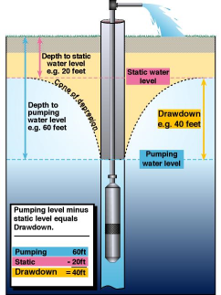
\includegraphics[width=0.75\linewidth, height=0.25\textheight]{WellDrawdownCalc}
%        \caption{Drawdown calculations}
%        \label{fig:prob1_6_1}
%    \end{minipage}








%\begin{figure}[h!]
%\begin{center}
%\includegraphics[scale=0.7]{Welldesign}
%\caption{Well construction}
%\end{center}
%\end{figure}
%\begin{figure}[h!]
%\begin{center}
%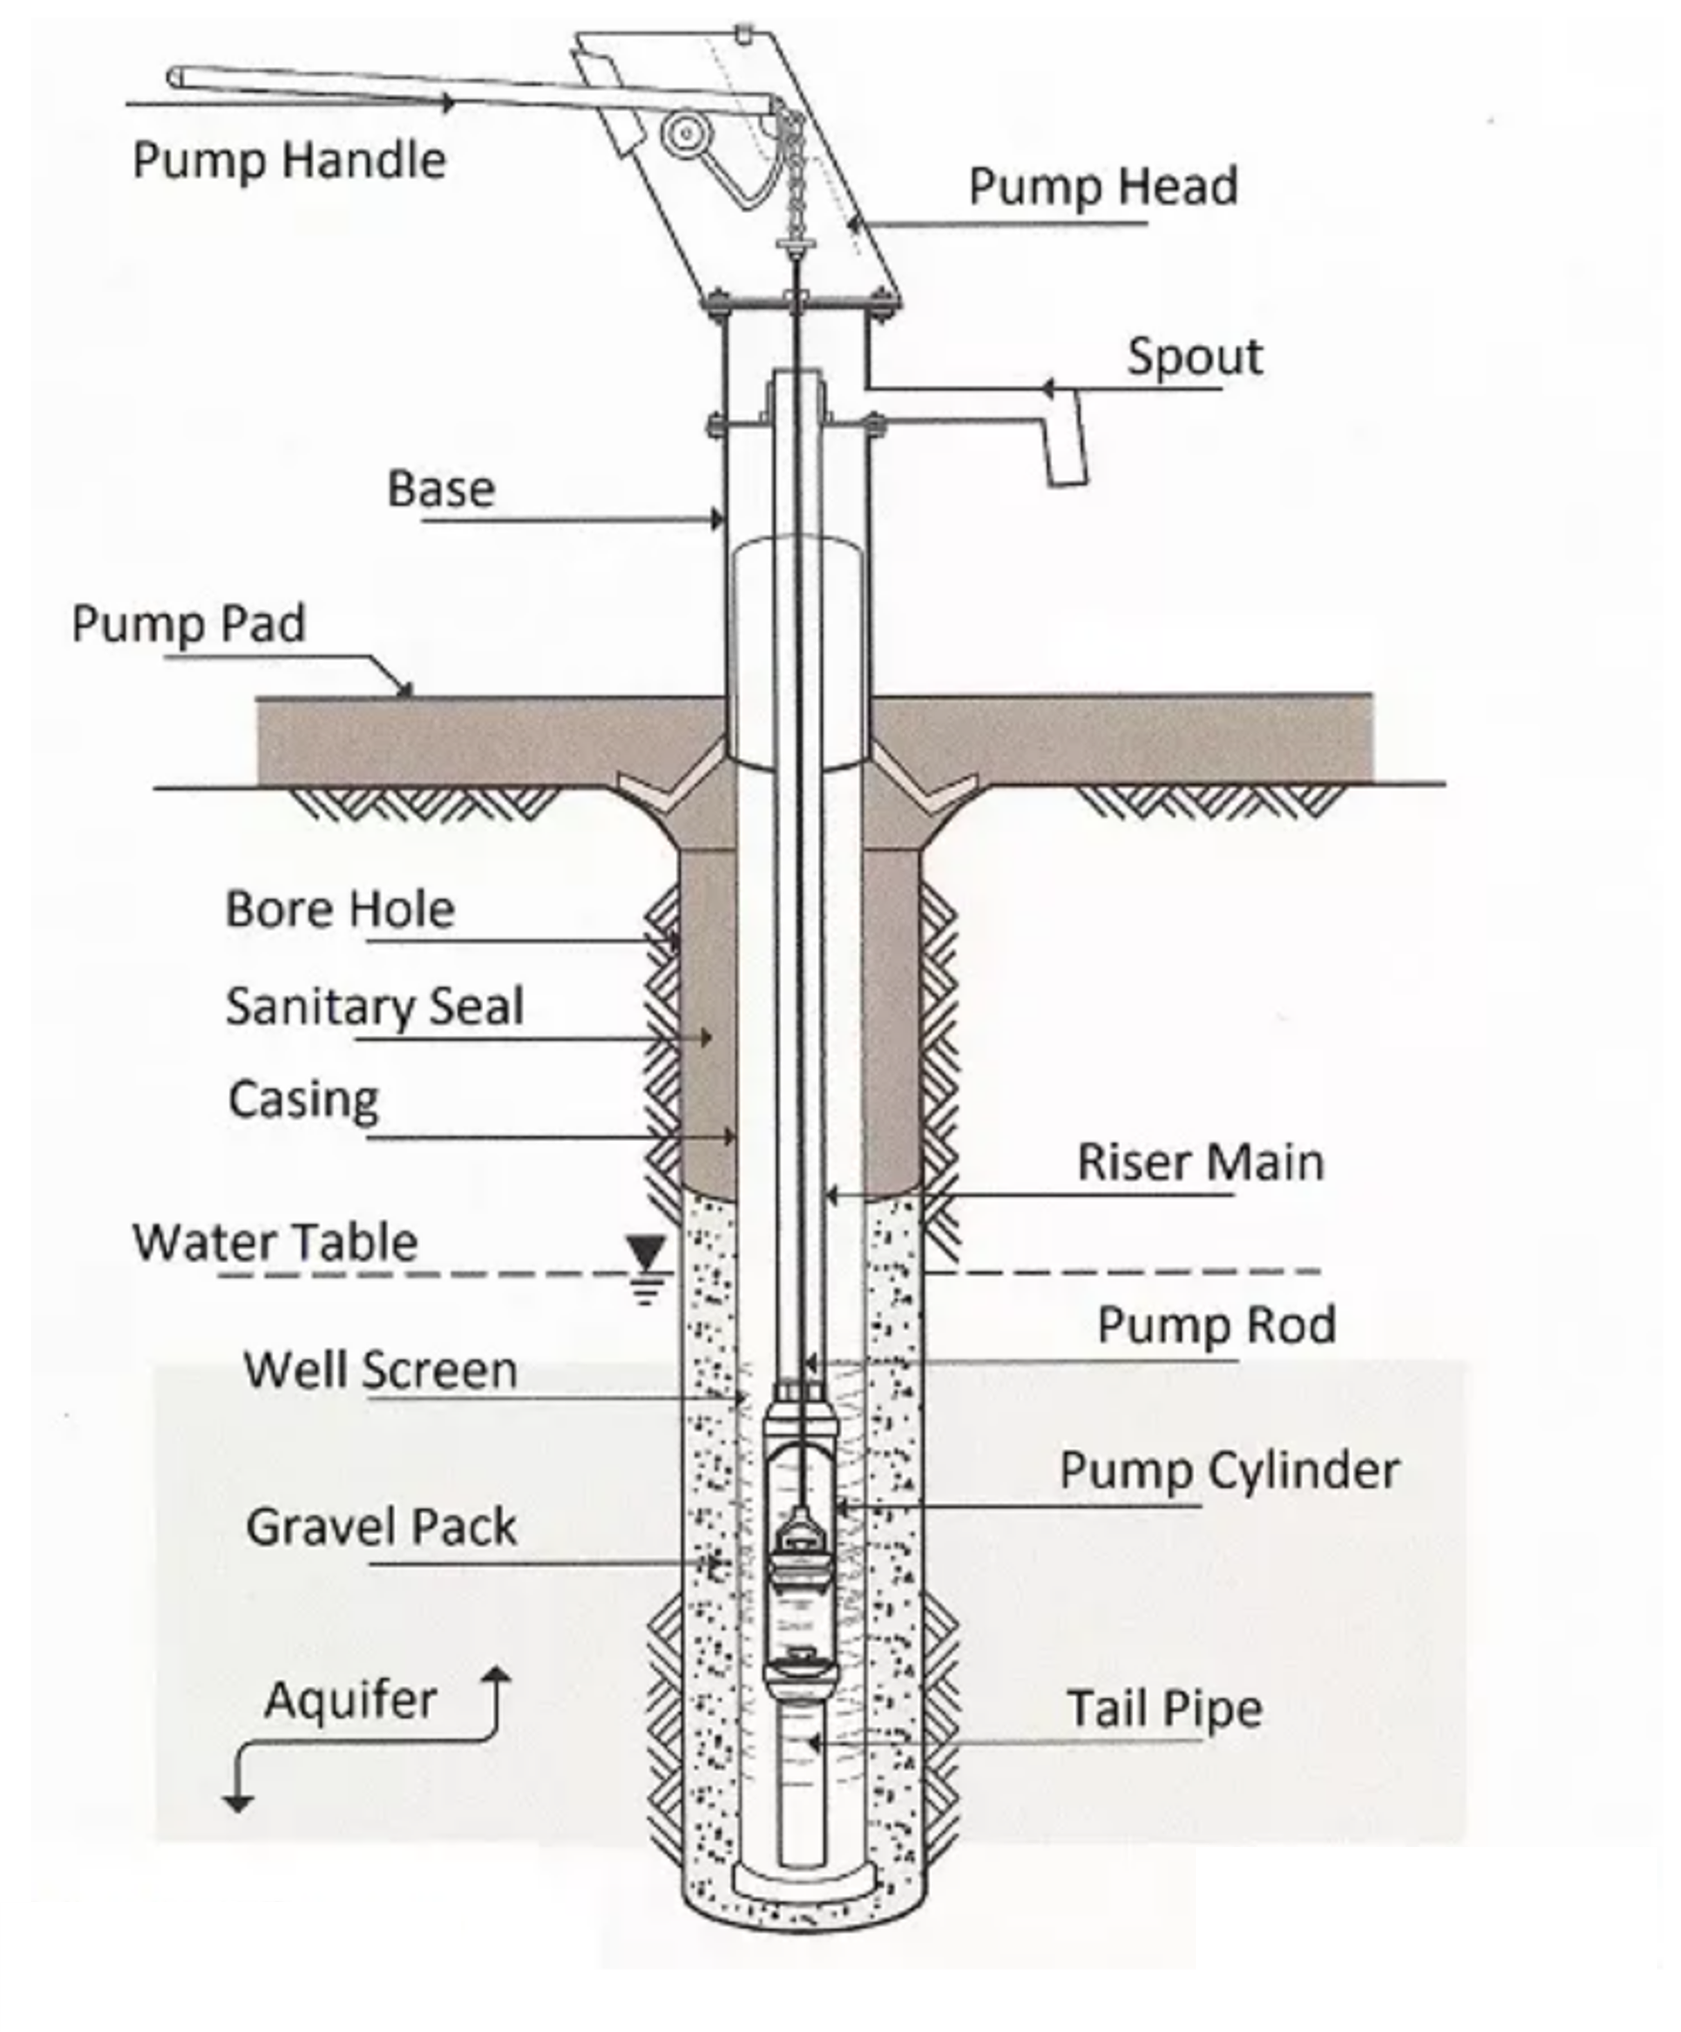
\includegraphics[scale=0.5]{Well}
%\caption{Well calculations}
%\end{center}
%\end{figure}
\item \ul{Recovery time} \index{Wells!Recovery time}is the amount of time required for the aquifer to stabilize at its static water level once pumping has stopped.
\end{itemize}
\begin{figure}[!htb]
    \centering
    \begin{minipage}{0.8\textwidth}
        \centering
        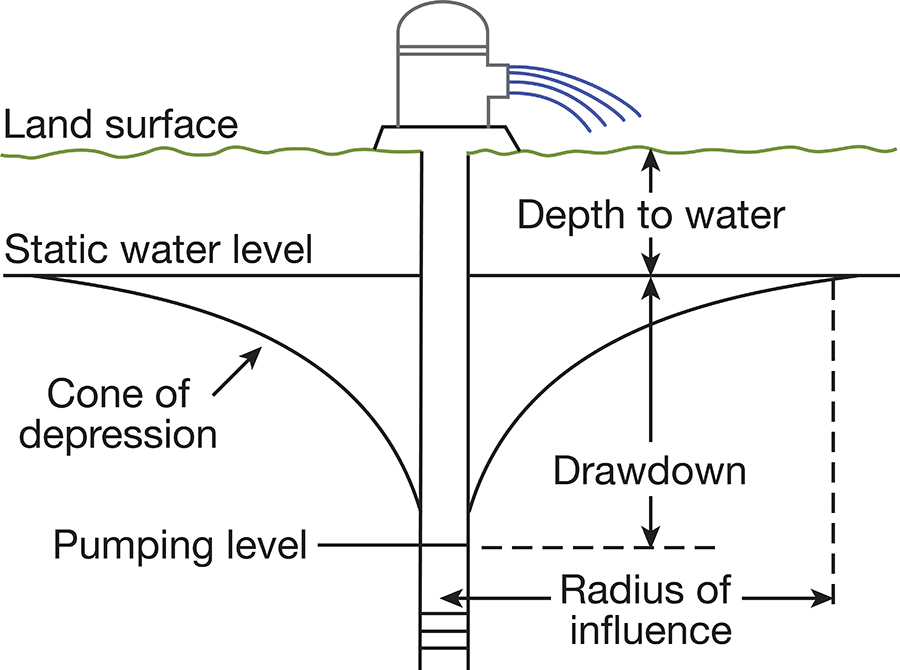
\includegraphics[width=0.6\linewidth, height=0.25\textheight]{WellTermsGraphic2}
        \caption{Well terms}
        \label{Well terms}
    \end{minipage}%
    \end{figure}


\textbf{Well types} \index{Wells!Well types}
\begin{itemize}
\item Wells are classified by method of construction of the well.
\item Well types \index{Wells!Types of wells}include:
\begin{itemize}
\item Dug wells \index{Wells!Types of wells!Dug,driven,drilled wells}:  These wells are typically:
\begin{itemize}
\item large diameter
\item 10-30 ft deep
\item hand-dug to the top layer of the aquifer.  
\item lined with stone or bricks
\end{itemize}
Dug wells levels fluctuate with seasonal variation of water table and has a high risk of contamination from nearby land activities.

\item Driven wells:  These wells are for reaching shallow waters about 30-50 feet deep and are made by driving a small diameter pipe.  Although the well is cased, it has a moderate to high evel of risk of contamination from nearby land activities.

\item Drilled wells:  Drilled well is the most common type of well used by public water systems.  These wells are constructed using a rotary-drilling machine and are hundreds of feet deep.  These wells have a continuous casing, which is commonly six-inches in diameter.  These wells are ideally suited to deep water bearing formations where larger yields are available. This type of well, when properly constructed offers good protection against contamination from the surface.
\end{itemize}

\end{itemize}

\textbf{Well Construction} \index{Wells!Well construction}\\
Elements of well construction include:\\
\begin{itemize}
\item \ul{Borehole} \index{Wells!Wells construction!Borehole} is the narrow shaft drilled to extract water from the aquifer.
item \ul{Well casing} \index{Wells!Well construction!Well casing} is the watertight plastic  or steel tube lining of the borehole.  It is generally 4-6" diameter and it is primarily to protect the borehole from caving in and to prevent surface water from entering the well.  The casing should extend at least 6 to 12 inches above the
well pad, depending on whether the well is located in a well house or out in the open, to prevent standing water from entering the well.
\item \ul{Well screen} \index{Wells!Well construction!Well screen}  is installed on the end of a well casing.  It supports the bore hole, and it reduces the amount of sand that enters the casing and the pump.
\item \ul{Gravel packer} \index{Wells!Well construction!Gravel packer} is a layer of gravel placed around the screen to reduce the amount of fine material from entering the well through the screen.  The gravel packing is usually three times the diameter of the well screen or a minimum of 4" thick.
\item \ul{Grout} \index{Wells!Wells construction!Grout} is cement or bentonite packing around the well casing to protect the well from surface water.  The grout is applied continuously from the surface upto the bottom where the borehole passes into the impermeable layer or upto the gravel packer.
\item \ul{Ground seal} \index{Wells!Well construction!Ground seal}is typically a reinforced concrete slab. This concrete is usually connected to the grout that extends down the well.
\item \ul{Sanitary seal}\index{Wells!Well construction!Sanitary seal} it seals the top of the casing and its primary function is to prevent well contamination.  The type of seal varies depending upon the type of pump being used.  For a well using a submersible pump, the sanitary seal is typically composed of a rubber-like material
placed between two pieces of metal. When bolts are tightened on the sanitary seal, the rubber is compressed and expands to seal against the casing and the pump discharge pipe.
\begin{figure}[h!]
\begin{center}
\includegraphics[scale=0.6]{Welldesign}
\caption{Well construction}
\label{Well construction}
\end{center}
\end{figure}
\end{itemize}
\subsection{Groundwater Under the Direct  Influence  of  Surface  Water}\index{Groundwater under the direct  influence  of  surface  water (GWUDISW)}
\begin{itemize}
\item Groundwater under the direct  influence  of  surface  water (\textbf{GWUDISW}) is the water which may be subject to contamination with pathogenic organisms from surface waters. 
\item GWUDISW is defined as:\\
Any water beneath the surface of the ground with significant occurrence of:\\
\begin{itemize}
\item Insects 
\item Other macroorganisms
\item Algae
\item Large diameter pathogens such as Giardia lamblia
\end{itemize}
\vspace{0.3cm}
or as:\\
\begin{itemize}
\item Any water beneath the surface of the ground with significant and relatively rapid shifts in water characteristics such as:
\begin{itemize}
\item Turbidity
\item Temperature
\item Conductivity, or
\item pH
\end{itemize}
that closely correlates to climatological or surface water conditions.     
\end{itemize}
\end{itemize}

\subsection{Surface water}\index{Surface water}
\begin{itemize}
\item Surface water is water that is open to the atmosphere and results from overland flow. It is also said to be the result of surface runoff. These are two ways of saying the same thing.
\item Examples of surface water include:
\begin{itemize}
\item Streams, Rivers, Lakes
\item Man-made impoundments - Reservoirs
\item Wells drilled next to or in a stream or river
\item Rain catchments
\end{itemize}
\item Surface waters are classified as either:  running waters which include streams, rivers and brooks; and quiescent waters which include lakes and reservoirs.
\
\item  A lake is where surface-water runoff (and maybe some groundwater seepage) have accumulated in a low spot, relative to the surrounding countryside.  Whereas a reservoir is a man-made lake that is created when a dam is built on a river. 
\item The exposure of surface waters to the atmosphere results in exposure to precipitation events, surface water runoff and contamination with micro and macroorganisms resulting from activities in their surrounding areas.

\item Changes in weather cause the natural flow of streams and rivers to vary greatly with time. Periods of excess flows and valley flooding may alternate with low flows or droughts.
\item  The role of water-storage reservoirs, also known as impoundments is to store water during periods of higher flows, thus preventing flood disasters, and then permit gradual release of water during periods of lower flows. 

\item Lakes and reservoirs can be classified into three categories \index{Surface water!Lakes and reservoirs classification} based upon their nutrient content:
\begin{itemize}\index{Eutrophic} \index{Mesotrophic} \index{Oligotrophic}
\item Eutrophic - rich in nutrient
\item Mesotrophic - moderate amount of nutrient 
\item Oligotrophic - little or no nutrient
\end{itemize}
\item In many locations, as the water temperatures decrease with increasing water depth, thermal stratification \index{Lake thermal stratification} - formation of distinct thermal layers, of lakes and reservoirs occur due to temperature related density changes which prevents the vertical mixing of water. 
\begin{enumerate} \index{Epilimnion} \index{Thermocline} \index{Hypolimnion}
\item Epilimnion - Suface layer of warm, light water (mixed by wind)
\item Thermocline or Metalimnion- Middle layer with rapidly changing temperature
\item Hypolimnion - Lowest layer of coldest and densest water. Hypolimnion usually has depletion of dissolved oxygen (DO) leading to fish kills for fish living at that depth.	·
\end{enumerate}

\begin{figure}
\begin{center}
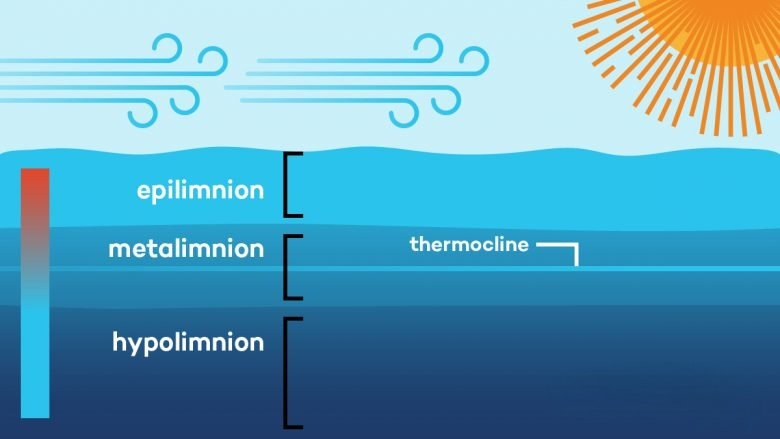
\includegraphics[scale=0.5]{ReservoirStratification}\\
\captionof{figure}{Lake/reservoir stratification}%\caption{}
\label{Lake/reservoir stratification}
\end{center}
\end{figure}
\item Destratification \index{Destratification} - can be natural by change in weather or by means such as aeration or mechanical agitation and mixing.
\item Lake turnover \index{Lake turnover}- During autumn and winter, top layer of water gets colder and denser and
sink to the bottom, water from bottom comes to the top causes the bottom sediments to be stirred	causing high turbidity in the water. It can also cause the heav metals (such as mercury and lead from the bottom of the reservoir become dispersed in the water.

\item Thus, water intakes are located at various levels in the reservoir to get the best possible quality of raw intake water possible at different times of the year.

\end{itemize}

\subsection{Advantages and disadvantages of surface water vs groundwater }\index{Advantages and disadvantages of surface water vs groundwater }
\begin{itemize}
\item Advantages of surface water with respect to groundwater:
\begin{itemize}
\item It is easily located. It takes no sophisticated equipment to find a surface water source.
\item In many parts of the US, considerable data is available on quantity and quality of existing surface water supplies.
\item Surface water is generally softer than groundwater, which makes treatment much simpler.
\end{itemize}
\item Disadvantages of surface water with respect to groundwater:
\begin{itemize}
\item Surface waters can be easily contaminated with microorganisms that cause waterborne diseases and chemicals that enter the stream from surface runoff and upstream discharges.
\item The turbidity of a surface water source often fluctuates with the amount of precipitation. Increases in turbidity increase treatment cost and operator time.
\item The temperature of surface water fluctuates with the ambient temperature. This makes it difficult to produce consistent water quality at a water treatment plant.
\end{itemize}
\item Advantages of groundwater with respect to surface water:\\
\begin{itemize}
\item Groundwater is not as easily contaminated as surface water.
\item The quality of groundwater, while not always as good as would be preferred, is stable throughout the year.
\item Groundwater sources are generally lower in bacteriological count than surface water sources.
\item Groundwater is available in most locations throughout the continental US and Alaska.
\end{itemize}
\item Disadvantages of groundwater with respect to surface water:\\
\begin{itemize}
\item Groundwater usually contains more minerals than surface water, including increased levels of hardness. Because groundwater is in contact longer with minerals, there is more time to bring them into solution.
\item Removal of groundwater normally requires a pump, thus increasing operation cost.
\item Groundwater is more susceptible to long-term contamination from fuel spills.
\item Groundwater supplies often have high levels of iron and manganese, thus increasing treatment cost and/or causing stains on plumbing and the clothing of customers.
\item Wells in the coastal areas are subject to salt water intrusion into the aquifer
and well. This contamination is difficult to predict and costly to treat.
\item Once a groundwater source is contaminated, it is difficult for it to recover. There is no easy way to remove the contaminants. Sources of contamination can be hidden from sight.
\end{itemize}
\end{itemize}
\begin{figure}
\begin{center}
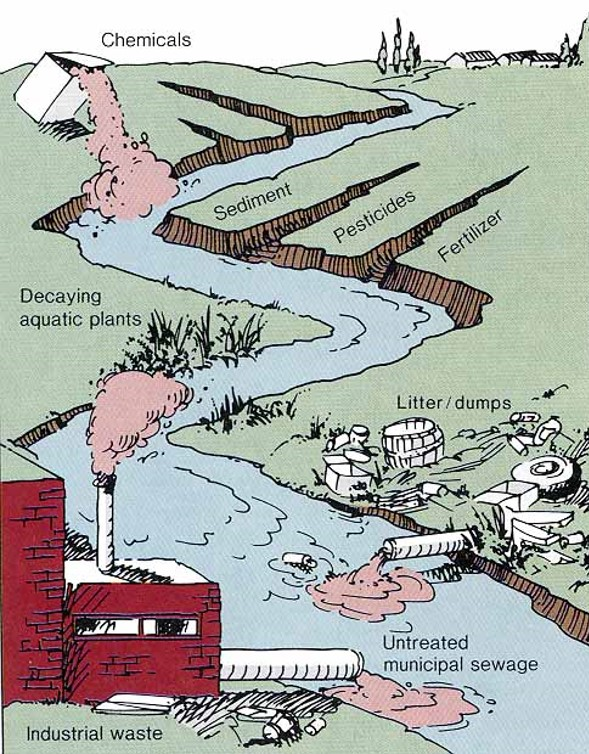
\includegraphics[scale=0.5]{WaterContamination}\\
\captionof{figure}{Sources of water contamination}%\caption{}
\label{Sources of water contamination}
\end{center}
\end{figure}
\subsection{Recycled water}\index{Recycled water}
\begin{itemize}
%\item Within the Water Cycle, there are many subcycles which can be regional or local.
%\item One such cycle is the local cycle which involves water use and reuse.\\
%\begin{figure}
%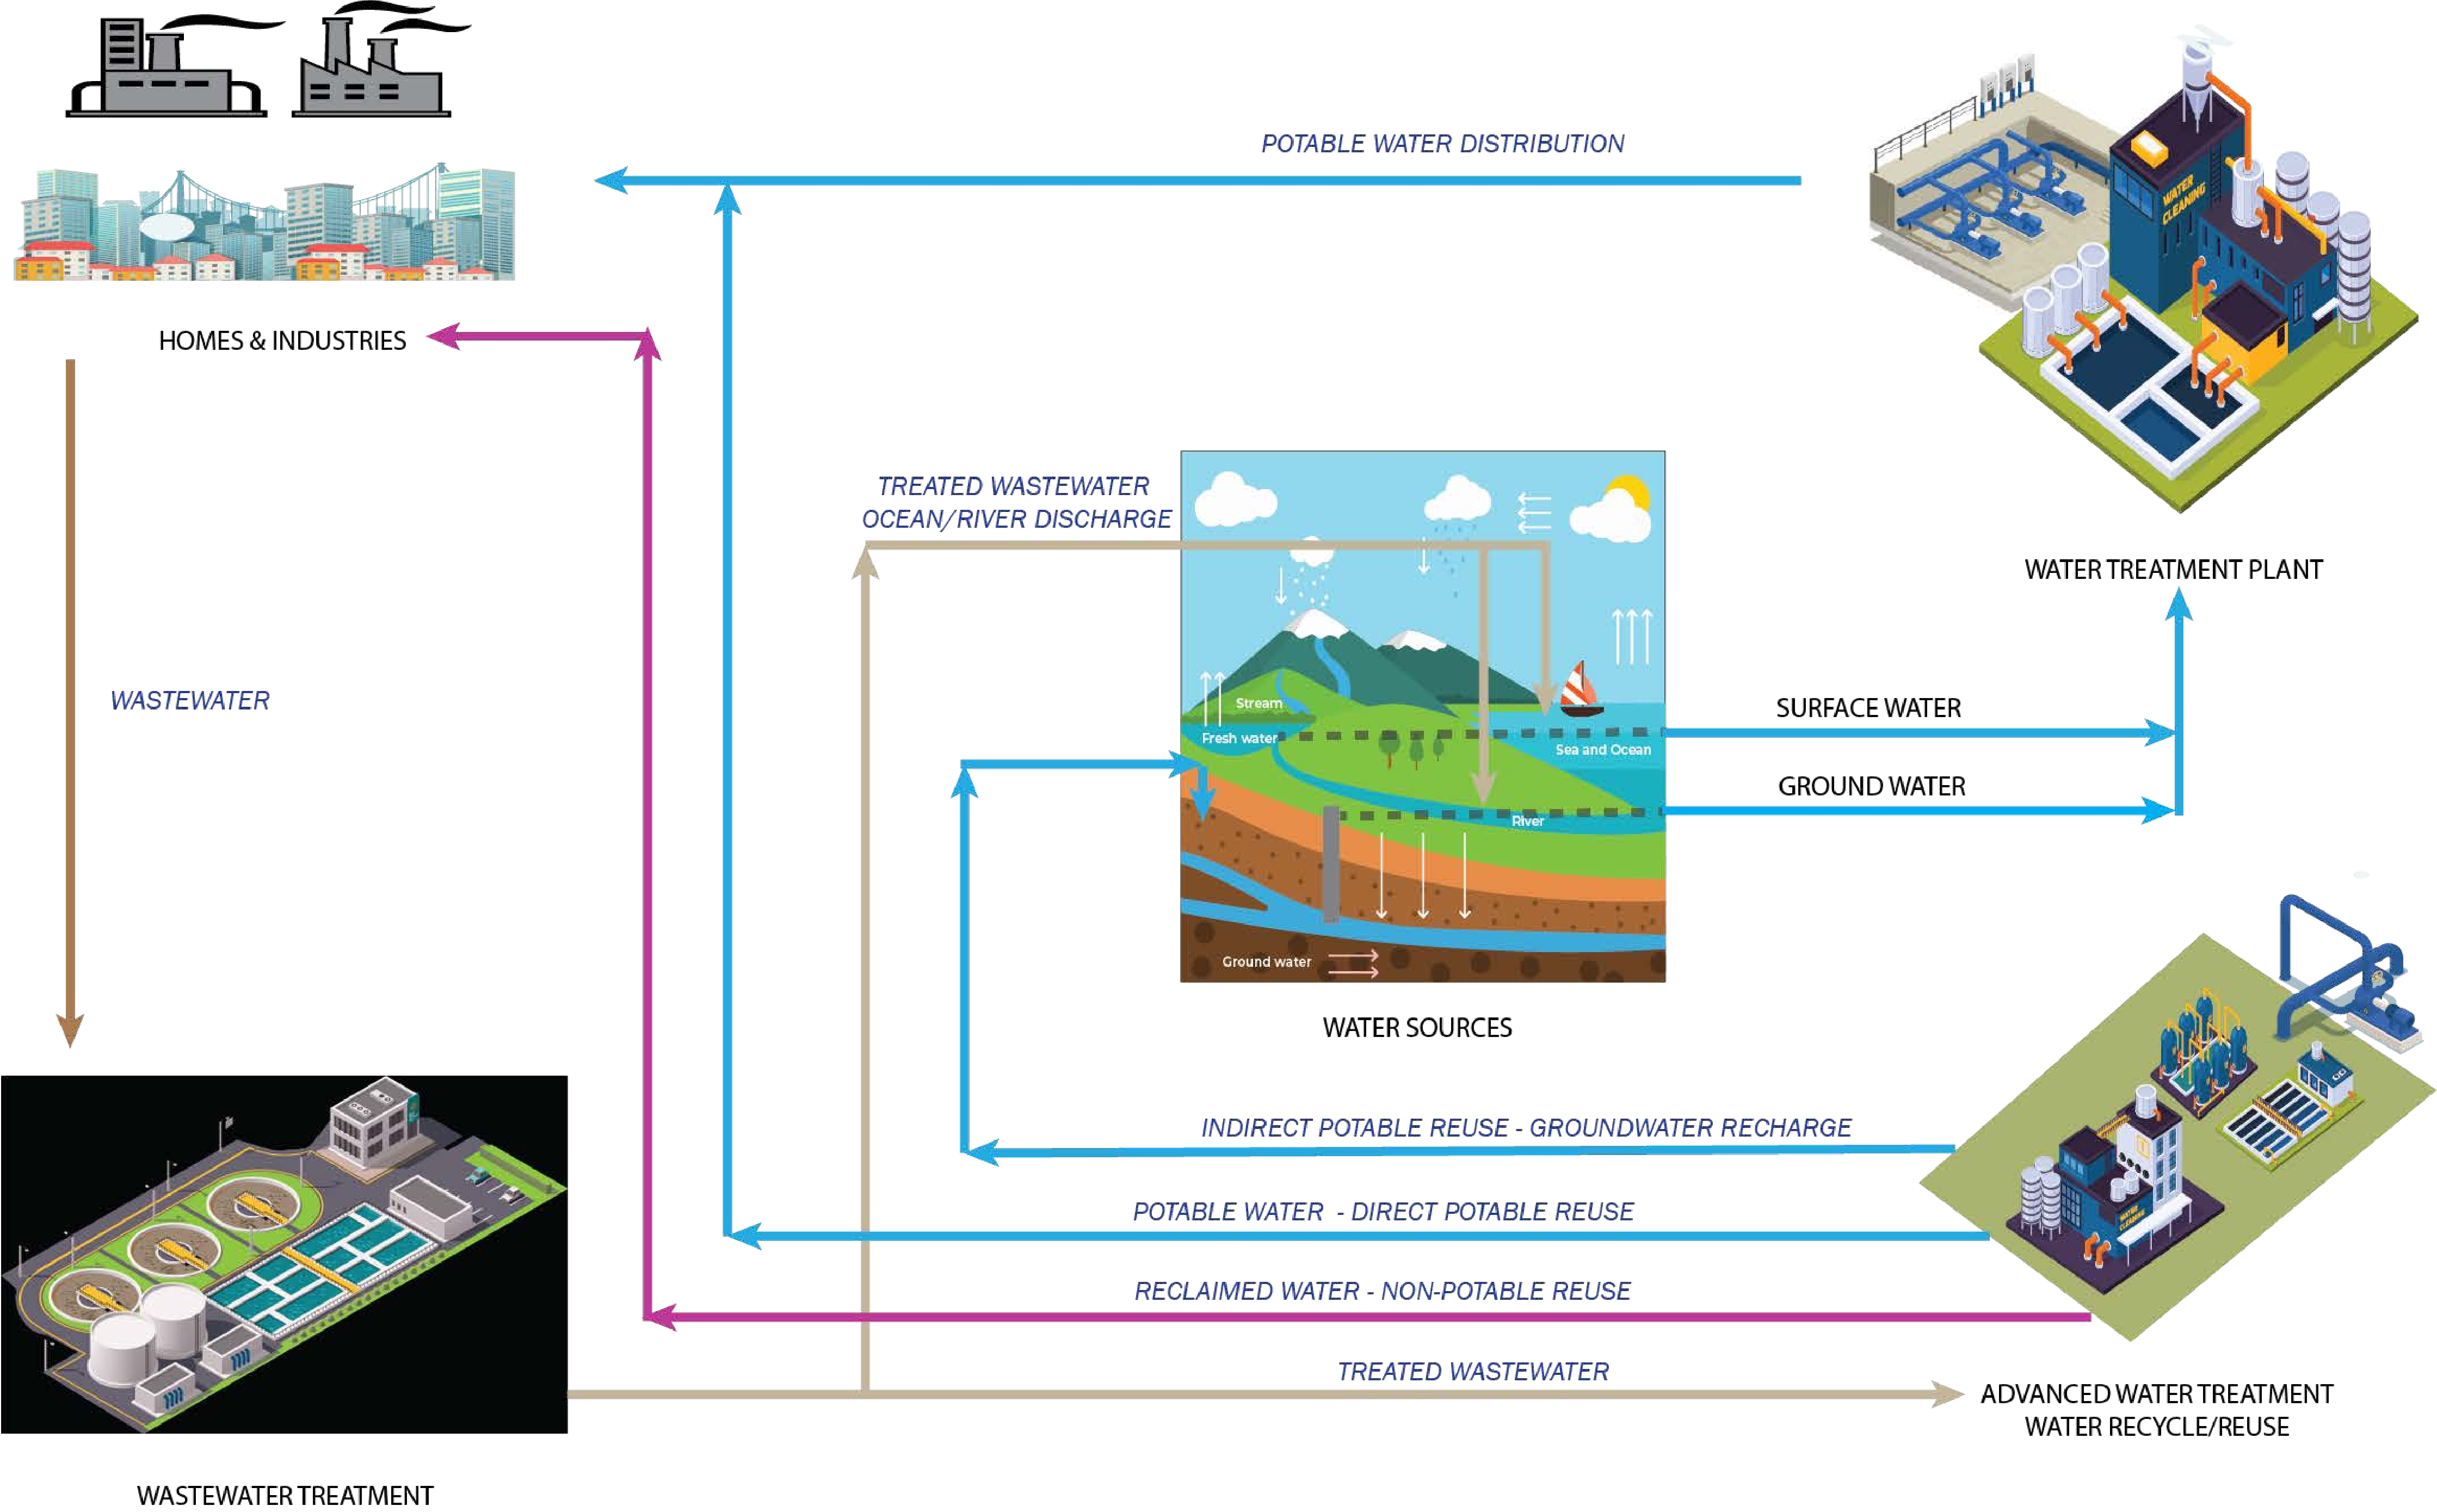
\includegraphics[scale=0.2]{Test4}\\
%\captionof{figure}{Water Use - Reuse Cycle}%\caption{}
%\end{figure}
\item Water reuse (also commonly known as water recycling or water reclamation) reclaims water from a variety of sources then treats and reuses it for beneficial purposes such as agriculture and irrigation, potable water supplies, groundwater replenishment, industrial processes, and environmental restoration.
\item Water reuse can provide alternatives to existing water supplies and be used to enhance water security, sustainability, and resilience.

\item Unplanned or de facto reuse refers to situations in which a source of water is substantially composed of previously-used water. An example of unplanned water reuse occurs when communities draw their water supplies from rivers, such as the Colorado River and the Mississippi River, that receive treated wastewater discharges from communities upstream.
\end{itemize}

\section{Water rights in California}\index{Water rights}
\begin{itemize}
\item If one takes water from a lake, river, stream, or creek, or from underground supplies for a beneficial use, California law requires that person to have a water right. The term “beneficial use” can refer to agricultural, mining, urban, industrial, or environmental uses.
\item In California, water rights law is administered by the State Water Resources Control Board (often called simply the State Water Board). 
\item A water right holder is entitled to a “reasonable” amount of water, which not only considers the purpose for which the water is being used but also the relative consumption of the water with regard to other water users in the system.
\item Two types of water are recognized by law in water with regard to the law: groundwater and surface water.
\item Groundwater is considered a local supply and there is little state regulation of its use,and consequently a state water right permit is not required for use of this water.
\item Primarily, landowners in California are entitled to pump and use a reasonable amount of groundwater from a basin underlying their land to put it to a beneficial, nonwasteful use.
\item The use of surface water is subject to state laws and regulations that control its development and use.
\item Most common surface water rights include:
\begin {enumerate}
\item Riparian rights \index{Water rights!Riparian rights}:\\
\begin{itemize}
\item Riparian rights are rights to the “reasonable and beneficial use of water on land that is adjacent to a watercourse - a lake, river, stream, or creek. 
\item A riparian right allows the landowner to take as much water as can be reasonably and beneficially used on the riparian property. 

\item Riparian owners must share with other riparian owners along the same water body, and they cannot waste water or unreasonably affect public trust resources. 

\end{itemize}

\item{Appropriative Rights} \index{Water rights!Appropriative rights}:\\
\begin{itemize}
\item Appropriative water rights are legal rights to use water from a water source, such as a river or stream, for beneficial purposes.
\item Someone who takes water for use on non-riparian land or who uses water that would not be there under natural conditions on riparian land, appropriates water.
\item These rights are typically granted based on the principle of "first in time, first in right," meaning that the first person or entity to beneficially use the water for a specific purpose has priority over later users. 
\item Appropriative water rights are common in regions where water is scarce and are often subject to regulations and permitting processes to ensure fair and sustainable allocation of water resources.
\item Water right permits and licenses issued by the State Water Board are appropriative water rights.
\item Appropriative water may be stored for later use, or held for diversion and beneficial use.
\end{itemize}

\item Prescriptive Rights \index{Water rights!Prescriptive rights}:\\
\begin{itemize}
\item A prescriptive right is a right that is acquired through adverse possession of someone else’s water right. It is similar to a “squatter’s right” to land.
\item Prescriptive rights originated in the context of conflicts between competing riparian users.
\end{itemize}

\end{enumerate}
\end{itemize}

\part{Module 5}
\input{Water Regulations Revised1.tex}
\part{Module 6}
\chapterimage{Week3Clarifier1.jpg}
\chapter{Water Treatment}

\begin{table}[H]
\begin{tabular}{| m{1cm} | m{15cm} |}
\hline
\multicolumn{2}{|l|}{\textbf{Expected   Range of Knowledge for Water Properties and Sources}}                                                                          \\ \hline
\multicolumn{2}{|l|}{\textit{Water   Distribution System Operator License Exams}}                                                                                      \\ \hline
D2 & Ability to   recognize normal operation of in-line sensors                                 \\ \hline
D2 & Ability to   troubleshoot a chemical feeder                                                \\ \hline
D2 & Knowledge of analysis   methods                                                            \\ \hline
D2 & Knowledge of chemical   feeder components                                                  \\ \hline
D2 & Knowledge of chemical   feeder types                                                       \\ \hline
D2 & Knowledge of required   reagents and standards                                             \\ \hline
D3 & Knowledge of   corrosion control techniques                                                \\ \hline
D3 & Knowledge of   principles of operation of cathodic protection devices                      \\ \hline
\multicolumn{2}{|l|}{\textit{Water   Treatment Operator License Exams}}                                                                                      \\ \hline
T1 & Ability to calculate   a dosage for a chemical feeder                                      \\ \hline
T1 & Ability to calibrate   and adjust a chemical feeder pump                                   \\ \hline
T1 & Ability to operate a   chemical feeder system                                              \\ \hline
T1 & Ability to replace   components of a chemical feeder system                                \\ \hline
T1 & Ability to set proper   chemical feed rate                                                 \\ \hline
T1 & Knowledge of chemical   feeder calibration and adjustment                                  \\ \hline
T1 & Knowledge of the   components of chemical feeder systems                                   \\ \hline
T1 & Knowledge of the   operation of chemical feeder systems                                    \\ \hline
T1 & Knowledge of basic   unit processes used in treating drinking water                        \\ \hline
T1 & Knowledge of   corrective actions to take when regulations are violated                    \\ \hline
T2 & Knowledge of   pretreatment procedures                                                     \\ \hline
T2 & Knowledge of head   loss effects on filters                                                \\ \hline
T2 & Knowledge of filter   surface washing methods                                              \\ \hline
T2 & Knowledge of   filtration mechanisms (absorption, adsorption)                              \\ \hline
T2 & Ability to choose an   appropriate disinfectant for a specific microbial problem           \\ \hline
\end{tabular}
\end{table}


\newpage



\begin{table}[H]
\begin{tabular}{| m{1cm} |m{15cm} |}
\hline
\multicolumn{2}{|l|}{\textbf{Expected   Range of Knowledge for Water Properties and Sources}}                                                                      \\ \hline
\multicolumn{2}{|l|}{\textit{Water   Treatment Operator License Exams (Continued)}}                                                                  \\ \hline
T2 & Knowledge of   chloramine chemistry                                                        \\ \hline
T2 & Knowledge of   disinfectant byproduct reduction procedures                                 \\ \hline
T2 & Knowledge of   TOC/Disinfection byproduct correlation                                      \\ \hline
T2 & Knowledge of   corrosion reduction methods                                                 \\ \hline
T2 & Knowledge of Best   Available Technology (BAT) for common water contaminants               \\ \hline
T2 & Knowledge of   effective removal techniques for common contaminants                        \\ \hline
T2 & Knowledge of hardness   removal processes                                                  \\ \hline
T2 & Knowledge of the   components of on-line analyzers                                         \\ \hline
T3 & Ability to recognize   and correct problems in gravity filters                             \\ \hline
T3 & Ability to recognize   and correct problems in multimedia filters                          \\ \hline
T3 & Knowledge of backwash   sequencing                                                         \\ \hline
T3 & Knowledge of filter   media types and uses                                                 \\ \hline
T3 & Knowledge of maximum   filtration rates                                                    \\ \hline
T3 & Knowledge of normal   and abnormal filter media conditions                                 \\ \hline
T3 & Ability to calculate   filter media volume and capacity                                    \\ \hline
T3 & Knowledge of iron and   manganese removal techniques                                       \\ \hline
T3 & Knowledge of the   aeration process                                                        \\ \hline
T3 & Knowledge of the   operation of blowers and compressors                                    \\ \hline
T3 & Ability to   discriminate between normal and abnormal operation of blowers and compressors \\ \hline
T3 & Knowledge of the   components of pressure gauges                                           \\ \hline
T3 & Ability to recognize   analytical interferences in on-line analyzers                       \\ \hline
T3 & Ability to repair or   replace defective parts of on-line analyzers                        \\ \hline
T3 & Knowledge of the   operation of on-line analyzers                                          \\ \hline
T3 & Knowledge of the   operation of an electrical generator                                    \\ \hline
T3 & Knowledge of the   components of an electrical generator                                   \\ \hline
T4 & Ability to conduct a   comprehensive performance evaluation of a filter                    \\ \hline
T4 & Ability to operate an   air scour system                                                   \\ \hline
T4 & Ability to perform a   filter assessment surveillance program                              \\ \hline
T4 & Ability to perform a   filter profile analysis                                             \\ \hline
T4 & Ability to recognize   and correct problems in granular activated carbon filters           \\ \hline
T4 & Knowledge of air   scouring systems                                                        \\ \hline
T4 & Knowledge of filter   media replacement requirements and techniques                        \\ \hline
T4 & Knowledge of filter   porosity                                                             \\ \hline
T4 & Ability to choose the   proper corrosion control chemical for a specific problem           \\ \hline
T4 & Knowledge   fluoridation chemicals                                                         \\ \hline
T4 & Knowledge of fluoride   chemistry                                                          \\ \hline
T4 & Knowledge of chemical   oxidation techniques and uses                                      \\ \hline
T4 & Knowledge of granular   activated carbon (GAC)                                             \\ \hline
T4 & Knowledge of nitrate   removal processes                                                   \\ \hline
T4 & Ability to replace   components of blowers and compressors                                 \\ \hline
T4 & Knowledge of the   components of blowers and compressors                                   \\ \hline
\end{tabular}
\end{table}
\newpage





\section{Background}\index{Treatment!Background}
\begin{itemize}
\item Purpose of water treatment is to provide safe drinking water that does not contain objectionable taste, odor or color and provide adequate quantities of water for domestic, commercial, industrial and fire protection needs.

\item All water produced by public water systems must be drinking water quality, even though only about 1\% of water produced is used for drinking and cooking.


\item Water may be treated differently in different communities depending on the quality of the source water that enters the treatment plant. The water that enters the treatment plant is most often either surface water or groundwater. Surface water typically requires more treatment and filtration than groundwater because lakes, rivers, and streams contain more sediment (sand, clay, silt, and other soil particles), germs, chemicals, and toxins than groundwater.

\item Even though U.S. tap water supplies are considered to be among the safest in the world, water contamination can still occur. There are many possible sources of contamination, including:
\begin{itemize}
\item Sewage releases
\item Naturally occurring chemicals and minerals (for example, arsenic, radon, uranium)
\item Local land use practices (for example, fertilizers, pesticides, livestock, concentrated feeding operations)
\item Manufacturing processes (for example, heavy metals, cyanide)
\item Malfunctioning on-site wastewater treatment systems (for example, septic systems)
\item In addition, drinking water that is not properly treated or that travels through an improperly maintained distribution system (pipes) may also create conditions that increase risk of contamination.
\end{itemize}

\item The purpose of water treatment is to condition, modify, or remove undesirable impurities and to provide water that is safe, palatable, and acceptable to users. Some regulations state that if the contaminants listed under the various regulations are found in excess of the Maximum Contaminant Levels (\textbf{MCLs}), the water must be treated to reduce the levels. 

\item Drinking water quality varies from place to place, depending on the condition of the source water from which it is drawn and the treatment it receives, but it must meet U.S. Environmental Protection Agency (\textbf{EPA}) regulations. Community water systems follow the rules set forth by the Safe Drinking Water Act (\textbf{SDWA}).

\item Many states enforce their own drinking water standards that are at least as protective as EPA’s national standards. The SDWA rules include guidelines for drinking water quality, water testing schedules, and water testing methods.

\item The level of treatment and treatment processes used are primarily dependent on the quality - level of contamination of the source water.

\item Generally speaking surface waters contain more contaminants compared to groundwater as surface waters are more exposed to contamination from runoffs etc.  
\item Although groundwaters are succeptible to contamination from seepage and soil percolation, the sediment layers help filter water naturally. 

\item The quantity and quality of surface water supplies vary more than groundwater, particularly seasonally.

\item If we assume that the water source used to feed a typical water supply system is groundwater, which is usually the case in the U.S., a number of common groundwater problems may require water treatment. Among these other problems are: bacteriological contamination, hydrogen sulfide odors, hard water, corrosive water,and iron and manganese.

\item Private wells, which are not regulated by the EPA, supply drinking water to over 15 million homes. Well owners are responsible for keeping their water clean and safe.



\item Some water supplies may contain radionuclides (small radioactive particles), specific chemicals (such as nitrates), or toxins (such as those made by cyanobacteria). Specialized methods to control or remove these contaminants can also be part of water treatment.

\item There are many treatment approaches when it comes to treating a range of problems that can occur in groundwater. Many of these methods use a combination of technologies. When considering the appropriate approach, it is important to note that each site should be treated case by case. Since every site offers a different history, background, and unique landscape. 

\section{Categories of treatment methods}\index{Categories of treatment methods}
Typical treatment methods used can be categorized as:

\begin{enumerate}
\item Biological\\
\begin{itemize}
\item Microbes based biological systems are used for nutrient and organic removals from drinking water
\item Typically the biological processes utilize the fixed biofilm - support medium on which the biomass is attached.
\item Some applications use suspended growth reactors where the biomass is suspended in the water being treated. 
\end{itemize}

\item Chemical\\
\begin{itemize}
\item Chemical oxidants are injected or mixed into groundwater to destroy contaminants upon contact. Chemical oxidants include oxygen gas, ozone, and other liquid chemicals.\\
\end{itemize}
\item Physical\\
Most common physical techniques are:\\
\begin{itemize}
\item Sedimentation:  Involves gravity settling of settleable particles by gravitational force from the water.
\item Filtration involves removal of pollutants by physical processes including straining, adsorbtion and absorption.
\item Dissolved air flotation or Degasification:  Utilizes pressurized air to remove dissolved gases is the process of removing dissolved gases from the water.

\end{itemize}



\end{enumerate}
\vspace{1cm}

\section{Source management}\index{Source management}
\begin{itemize}
\item When options are available, source management implies effectively managing water sources, to ensure the intake of best possible quality of water from a regulatory compliance and treatment optimization perspective.
\item Examples of source management include:
\begin{itemize}
\item For systems using lake or reservoir sources, selecting the optimum depth from which to draw water depending on the water quality during that time of year or for other reasons (e.g. algal bloom,
storm upsets, etc).
\item Systems that have multiple sources may consider blending or alternating surface and ground
water sources to attain the best blended raw water for compliance. If blended prior to treatment, all water must be treated to surface water standards.
\end{itemize}
\end{itemize}

\section{Surface water treatment processes}\index{Surface water treatment processes}
\subsection{Typical surface water treatment process} \index{Typical surface water treatment process}
\begin{enumerate}
\item Water is withdrawn from a lake, reservoir or river at the intake
\item It is screened to remove debris
\item Water then enters the flash mixing tank where coagulants and other chemicals are added
\item Then it is divided into the flocculation basin
\item After flocculation, the water enters the settling basins where solids are removed
\item Filtration then removes particles that are too small to settle by gravity
\item The water is disinfected using some form of chlorine
\item Other chemicals such as fluoride, phosphate corrosion inhibitors or pH adjustment chemicals may be added
\item After a minimum detention time, the water may be pumped to the distribution systems Other processes may occur, such as pre-oxidation or activated carbon treatment.
\end{enumerate}

\begin{figure}[h]
\begin{center}
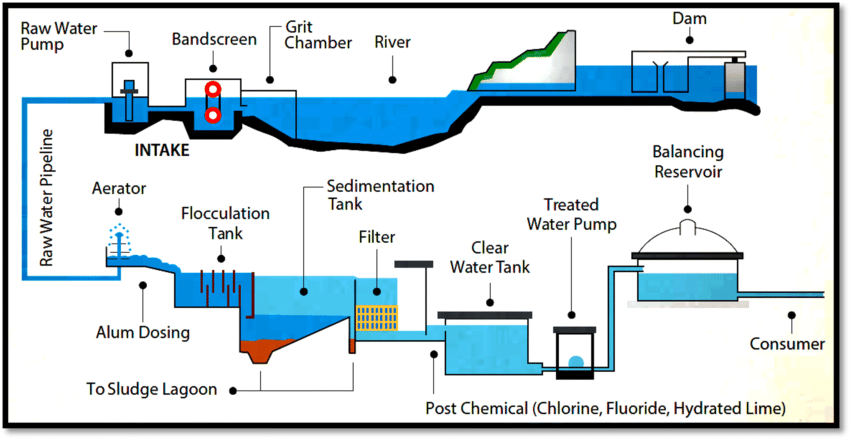
\includegraphics[scale=0.5]{WaterTreatment_9-01}
\caption{Conventional water treatment} \index{Conventional water treatment}
\end{center}
\end{figure}
\subsection{Source water treatment}\index{Source Water Treatment}
\begin{itemize}
\item Source water treatment in reservoirs or lakes includes treatment to contain algae growth.
\item Algal bloom is a sudden large increase in algae caused by weather or by nutrients. 
\item Reasons for controlling algae:
\begin{itemize}
\item Taste and odor problems
\item Shortened filter runs
\item Changes in pH - increases during the day, decreases at night
\item When algae dies, causes depletion of dissolved oxygen (DO)
\item Organic loading which is DBP pre-cursor resulting in TTHMs.
\end{itemize}
\item Algaecide such as blue stone, copper sulfate (CuSO$_4$) is used to control algae. 
\item Action level for copper is 1.3 mg/L·	·

\item Copper sulfate dose is usually specified in terms of pounds/acre. 
\item 5.4 lbs/acre is common dosage - the rate of application is based on the surface area of the reservoir not the volume
\item For water with alkalinify of higher than 150 mg/L, citric acid has to be mixed with CuSO$_4$ for it to be effective
\item Applying far more copper sulfate than necessary is uneconomical and ecologically undesirable. Excessive amounts of copper can kill fish and other bottom organisms, and copper tends to accumulate in bottom sediments. 
\end{itemize}
\subsection{Screening}\index{Screening}
\begin{itemize}
\item River water (the source of water used in our discussion) frequently contains suspended and floating debris varying in size from small rags to logs. Screening is usually the first major step where by large and suspended debris in the source water including sticks, leaves etc. is removed from the water before it enters the plant. 
\item Removing these solids is primarily to prevent damage to downstream equipment including pumps, prevent deposition of this debris in open channels or pipes, or in treatment processes.
\item The most important criteria used in the selection of a particular screening system for are the screen opening size and flow rate. Other important criteria include costs related to operation and equipment, plant hydraulics, debris handling requirements, and operator qualifications and availability. 
\item Depending on the characteristics of the source water, variety of screening devices including trash rakes, bar screens and wire mesh screens may be used. Very small screens can be used to screen out elements including algae in the water.
\item Typical screening devices used include:
\begin{itemize}
\item Trash Screens (Rakes) - used to remove rough or large debris.  The bar spacing in Rakes range from 1.5 to 4 inches.
\item Traveling Water Screens (Bandscreens) - these are placed in a channel of flowing water to remove floating or suspended debris.
\begin{figure}[h]
\begin{center}
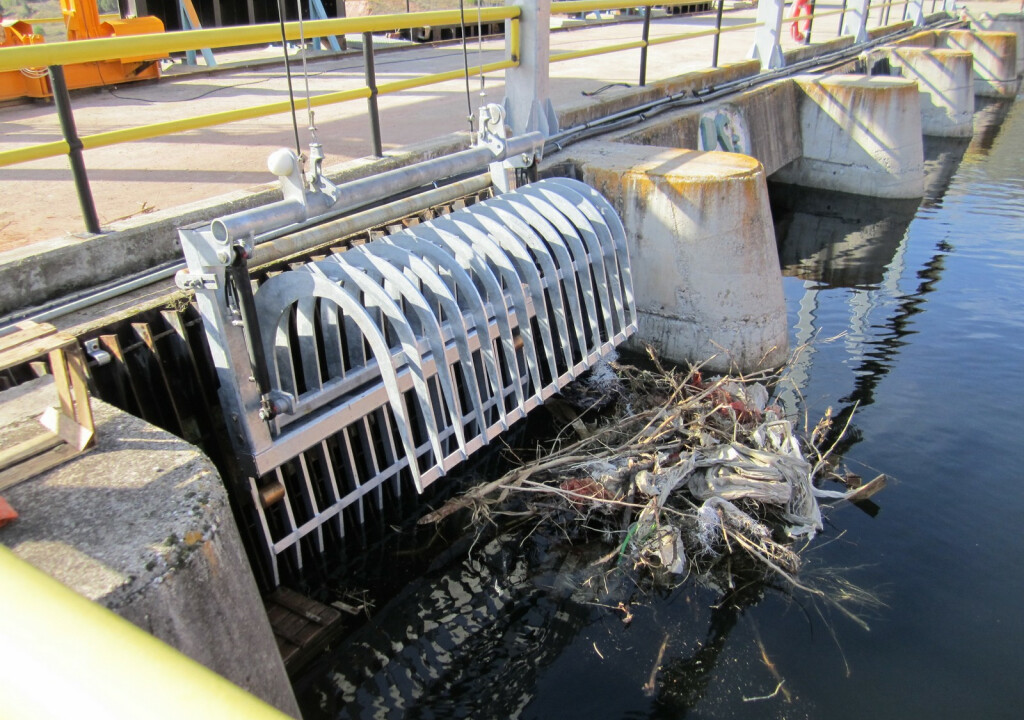
\includegraphics[scale=0.25]{TrashRakes}
\captionof{figure}{Trash rake}
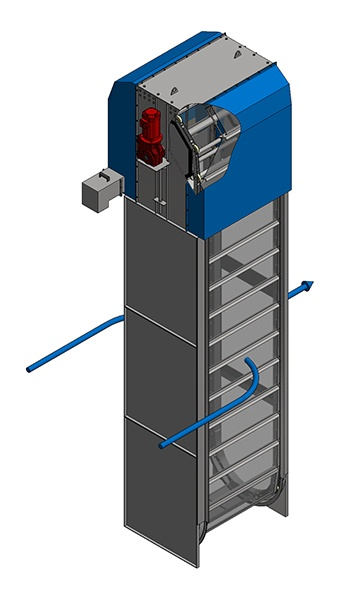
\includegraphics[scale=0.4]{TravellingScreen}
\captionof{figure}{Band screen}
\end{center}
\end{figure}
\end{itemize}

%\begin{center}
%\tcbox{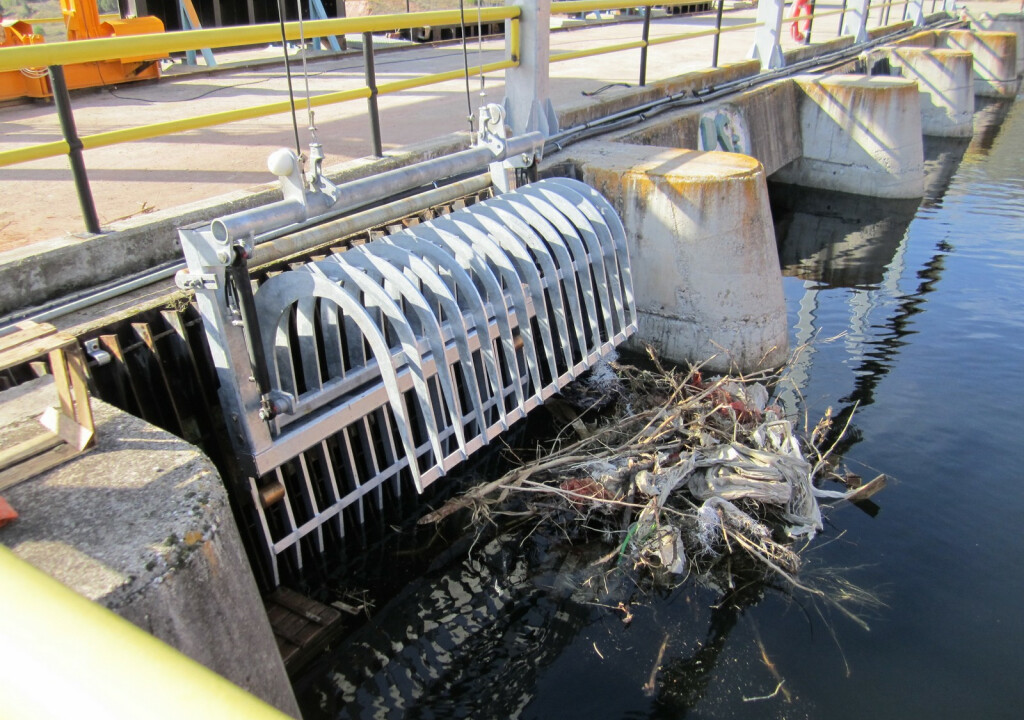
\includegraphics[width=6cm]{TrashRakes}}
%Trash Rakes
%\tcbox{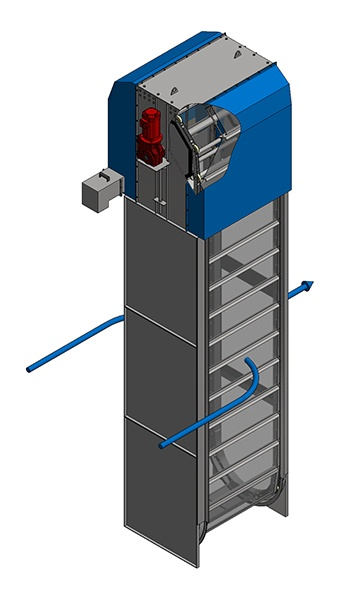
\includegraphics[width=6cm]{TravellingScreen}}
%\end{center}


\end{itemize}

\subsection{Coagulation and flocculation}\index{Coagulation and flocculation}
\begin{itemize}
\item A significant amount of suspended particles in the raw water are too small to be filtered or settled out in the sedimentation basin.  These particles, termed as colloids are non-settleable solids and include organic matter, silt, clay.
\item These particles impart turbidity and color to the water and may harbor pathogens and typically carry a negative electrostatic charge on its surface - negative \textbf{zeta potential}.  The like surface charge on these particles cause electrostatic repulsion (particles keep bouncing off one another) which makes these particles difficult to settle. 
\item Coagulation and flocculation are sequential processes both of which involve chemical addition.
\item For coagulation, either metal salt type coagulant - typically an aluminum salt such as alum or aluminum sulfate or an iron salt such as ferric or ferrous chloride or sulfate, polyaluminum chloride or a organic coagulant such as polyDADMAC or polyamine is used. The coagulant helps coalesce the non-settleable solids into larger particles.
\item Sodium aluminate is often used as an aide to alum coagulation particularly for cold water and during lime softening.
\item Coagulation is affected by changes in the water's pH, alkalinity, temperature, time, velocity and zeta potential.

\item The effectiveness of a coagulant is generally pH dependent. Water with a color will coagulate better at low pH (4.4-6) with alum.

\item Alkalinity is needed to provide anions, such as (OH$^-$) for forming insoluble compounds to precipitate them out. It could be naturally present in the water or needed to be added as hydroxides, carbonates, or bicarbonates.  Generally 1 part alum uses 0.5 parts alkalinity for proper coagulation.

\item The higher the temperature, the faster the reaction, and the more effective is the coagulation. Winter temperature will slow down the reaction rate

\item The coagulation process requires rapid mixing of the water upon the addition of the coagulant followed by a sufficient contact time prior to the flocculation step.
\item The flocculant which is added after the coagulation step is to make even larger, more compact and settleable - \textbf{floc}, from the coagulated solids.
\item Flocculants are typically long chain organic compounds - polymers with charged end groups.  \textbf{anionic polymers} have a negative end group whereas \textbf{nonionic polymers} have balanced - positive and negative end groups.
\item For the floc formed to remain intact, the polymer is gently "folded in" with the coagulated solids.  The flocculation is done in a flocculator which have a detention time of 5 -30 minutes and the water is mixed with the polymer using slow moving paddles.
\item Coagulant aids - chemicals which aid in the coagulation process and strengthening the flow include:
\begin{itemize}
\item Alakalinity enahncers - lime, Soda ash, caustic soda and sodium bicarbonate.
\item Weighting agents - calcimu carbonate and bentonite clay.  These are used in waters which are low in tubidity and high in color which under normal condition would have formed weak, slow settlling floc.
\item Activated sililca - sodium silicate activated by hypochlorous acid is often used as a coagulant aid with alum.
\end{itemize}


\end{itemize}

\item These will usually be used in conjunction with a primary coagulant such as ferric chloride, ferric sulfate, or alum.

\vspace{0.6cm}

\vspace{0.6cm}
\begin{figure}[H]
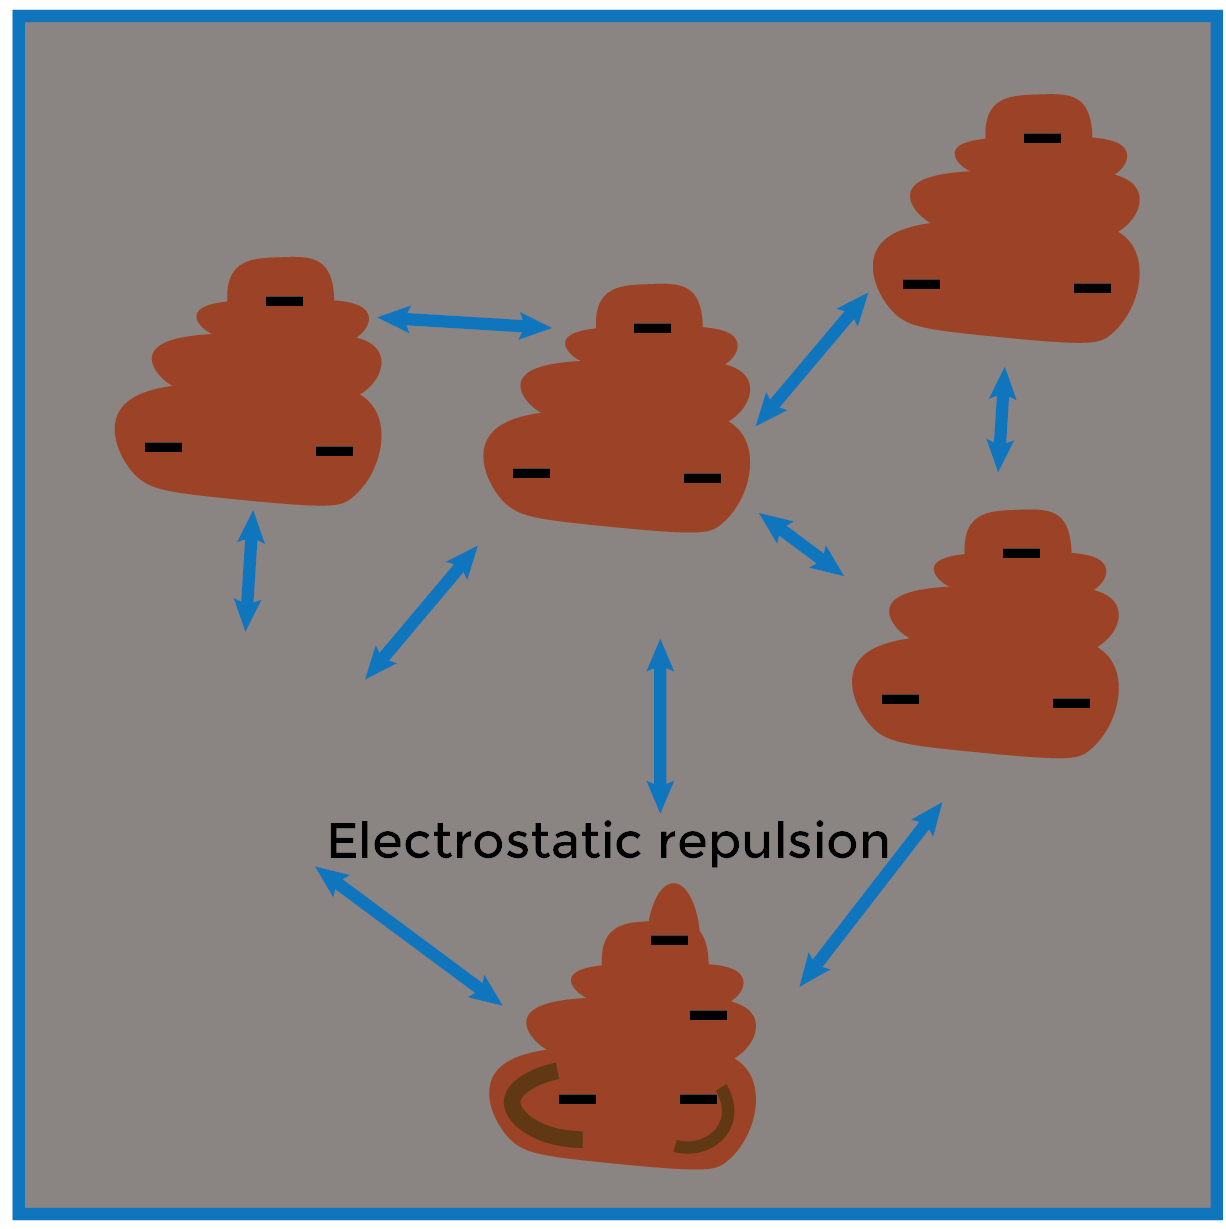
\includegraphics[scale=.13]{CEPTInitial} \hspace{0.7 cm}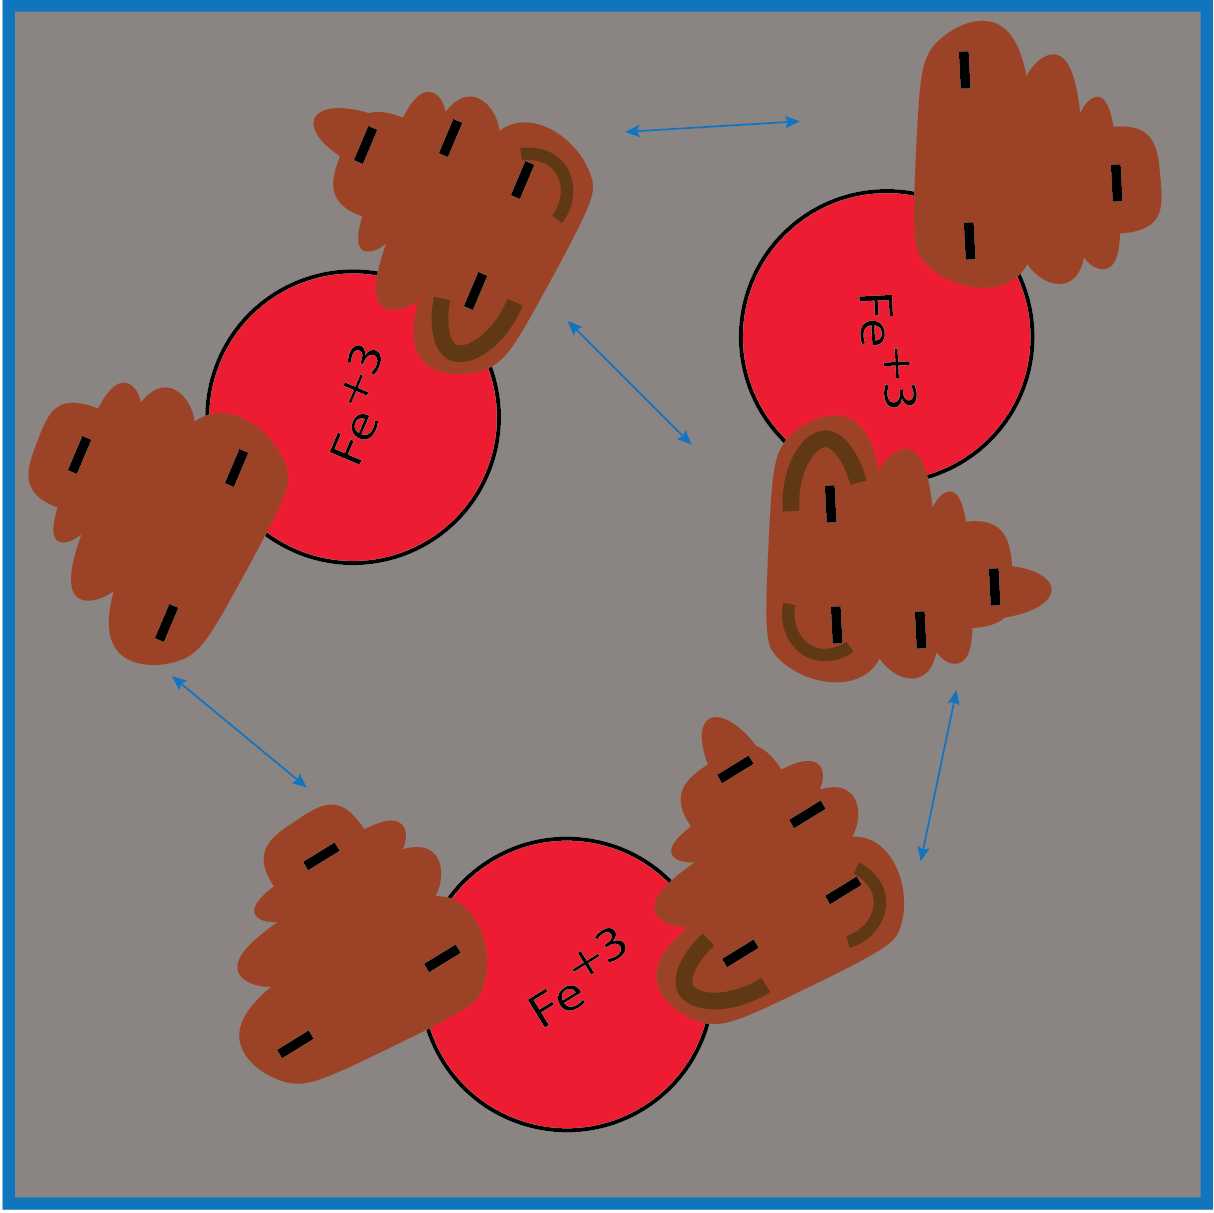
\includegraphics[scale=.13]{CEPTCoagulation}\hspace{0.7 cm}
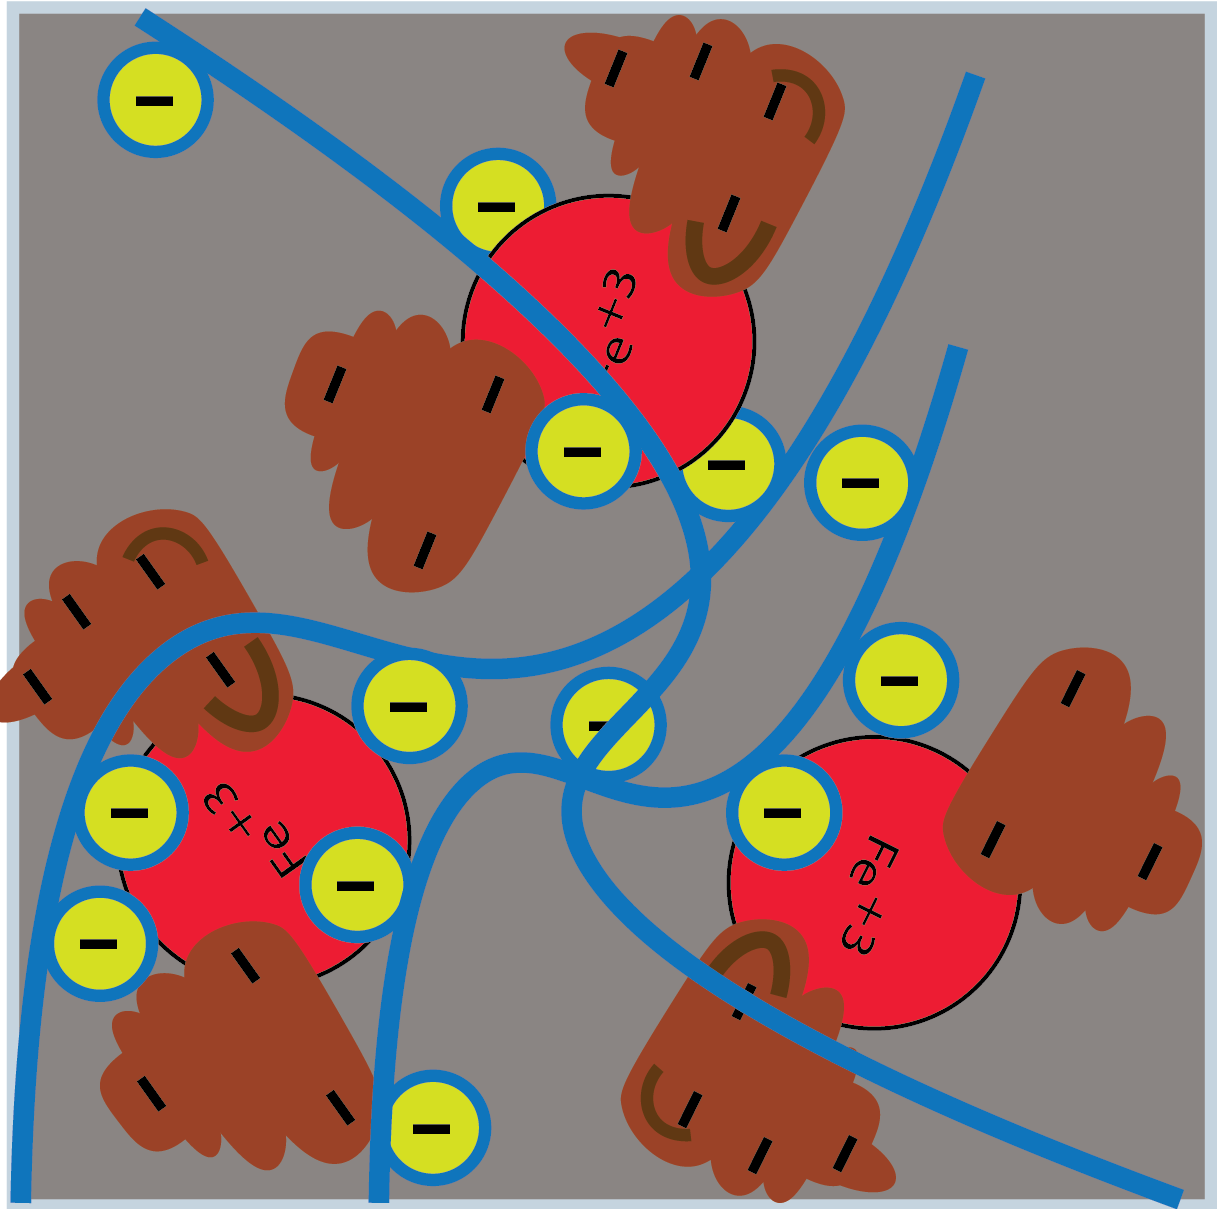
\includegraphics[scale=.13]{CEPTFlocculation}\\
\hspace{0.8cm} \textbf{Untreated Water}\hspace{2.4 cm}\textbf{Coagulation}\hspace{3 cm}\textbf{Flocculation}\\	
\caption{Coagulation-flocculation graphic}
\label{Coagulation-flocculation graphic}
\end{figure}

\item Determining the amount and type of coagulant used changes based on a variety of process conditions and quality of water. For example, a heavy rain will greatly impact the influent, or raw, water in a municipal treatment plant.

\item The jar test is a standard method in which various amounts of coagulant and flocculation times are tested on a raw water sample. There are multiple samples to test before implementation into a larger volume of the water treatment process.

\begin{figure}[h]
\begin{center}
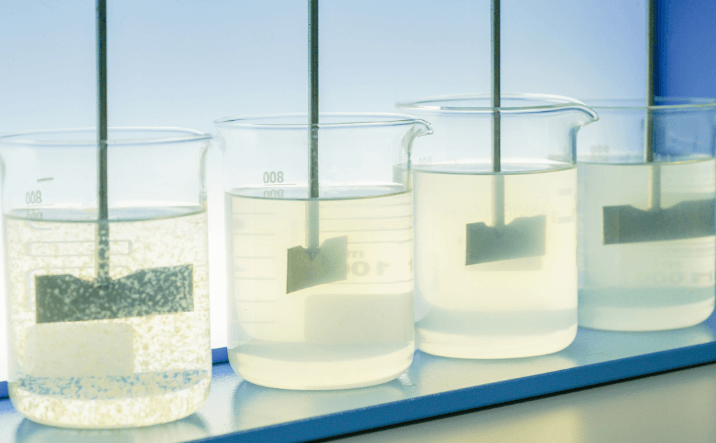
\includegraphics[scale=0.2]{JarTest}
\caption{Jar testing}
\label{table:Jartesting}
\end{center}
\end{figure}	

\end{itemize}
\subsection{Clarification/sedimentation}\index{Clarification/sedimentation}
\begin{itemize}
\item Clarification, or sedimentation, is the third step in conventional water treatment, after coagulation and flocculation and before filtration.
\item In the sedimentation basin the flocculated particles settle out under the influence of gravity.
\item In conventional sedimentation basins the solids drop out (settle) as the water slowly flows across the basin from the influent to effluent end.
\item Sedimentation basins are designed to create conditions in which the water flows very slowly through the basin, with minimal turbulence.
\item Conventional sedimentation basins are typically rectangular or cylindrical concrete or steel vessels which incorporate a horizontal flow of water.
\end{itemize}

			\begin{center}
				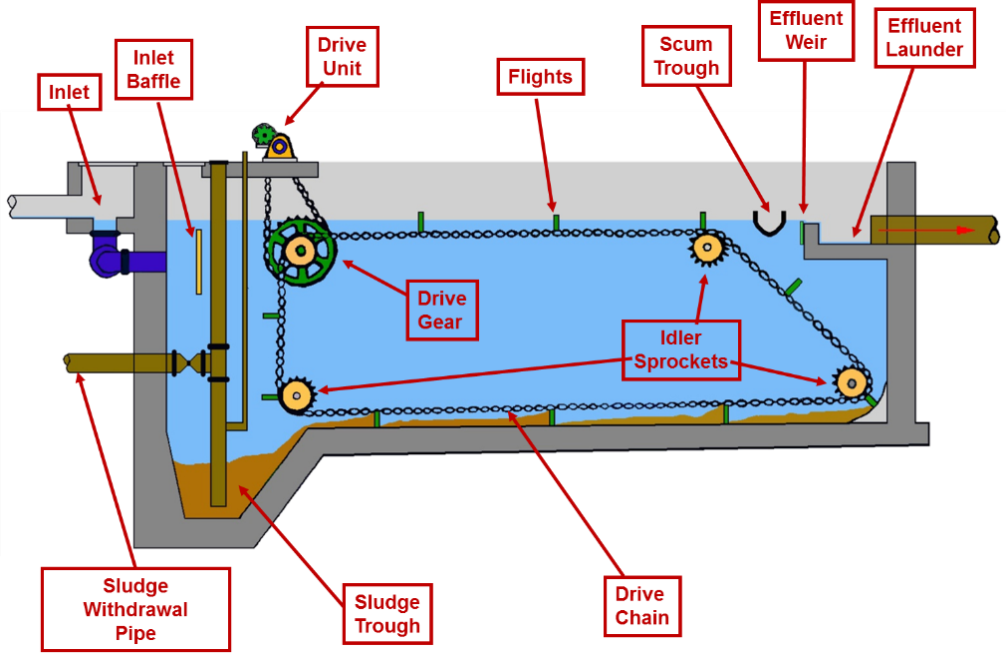
\includegraphics[scale=0.9]{RectangularClarifier}\\
				Cross section of a Rectangular Clarifier\\

				
\includegraphics[scale=0.1]{Blank}\\
				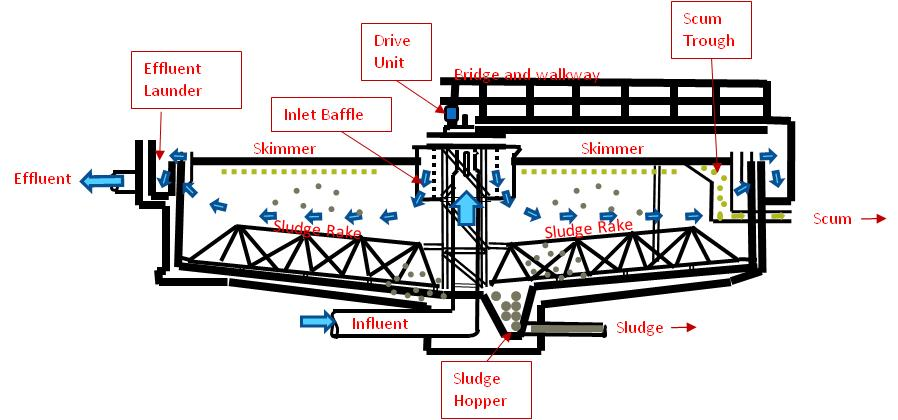
\includegraphics[scale=0.6]{CircularClarifierAI}\\
				Schematic cross section of a circular clarifier\\
				%\includegraphics[scale=0.1]{Blank}\\
				%\includegraphics[scale=0.65]{CircularClarifier3}\\
				%Cross section of a circular clarifier\\
			\end{center}
				%\includegraphics[scale=0.03]{Blank}\\


\subsubsection{Clarifier Zones}\index{Clarifier Zones}		
	\begin{itemize}
		\item Inlet Zone: is where the water enters the end of a rectangular tank, or the center of a circular or square tank. The Inlet Zone is designed to accomplish two objectives:
			\begin{enumerate}
				\item Reduce the velocity (dissipate 									energy in the incoming water).  This is accomplished by the inlet baffle.
				\item Distribute the flow evenly using baffles in front of the influent baffle.
			\end{enumerate}
				
		\item Settling Zone: This is the largest portion of the tank where the water is flowing very slowly allowing the solids to settle.  The clarifier is said to be short circuiting if 		the velocity of the water is greater in some sections than in others. The water passing through the higher velocity region will have a reduced detention time and settleable solids will carry through with this water as it exits the clarifier.
		\item Sludge Zone: Sludge zone is the bottom of the tank where the 	settled solids collect and compact. Sludge rakes push the sludge to one end or the center of the tank so that it can be pumped out. 
		\item Skimming Zone: The skimming zone is at the surface of the tank for removing scum removing
		lighter solids which float to the surface.  
		\item Outlet Zone: This is the part of the clarifier where the settled water leaves the clarifier.  A channel called the effluent launder collects the effluent flow and directs it to the clarifier effluent piping. Weirs are installed along the edge of the effluent launder channel to skim the water evenly off the surface of the tank. 
		\end{itemize}


\subsection{Filtration}\index{Filtration}
\subsubsection{Process Basics}\index{Process Basics}
\begin{itemize}
\item The SWTR requires the filtration of surface water and groundwater under the direct influence of surface water.
\item Filtration is the mechanical removal of turbidity particles by passing the water through a porous medium, which is either a granular bed or a membrane.
\item The process of filtration involves straining, settling, and adsorption.
\item Filtration does not remove dissolved solids and by itelf is not effective for the removal of bacteria.
\item In filtration, solids are removed physically by:
\begin{itemize}
\item Straining – trapping particles, and 
\item Adsorption.
\end{itemize}
\item The filtration based treatment process can be either:
\begin{enumerate}
\item Conventional - which is a four step treatment process that consists of the treatment steps of coagualation, flocculation, sedimentation and rapid sand filtration.  
\item Direct - where the sedimentation step is omitted. It is for areas with high quality of water and allows for cost and space savings by eliminating the need for sedimentation basins.  
\end{enumerate}
\begin{figure}[H]
\begin{center}
\includegraphics[scale=0.75]{ConventionalFiltration}\\
\captionof{figure}{Conventional filtration}%\caption{}
\label{Conventional filtration}
\end{center}
\end{figure}

\begin{figure}[H]
\begin{center}
\includegraphics[scale=0.75]{DirectFiltration}\\
\captionof{figure}{Direct filtration}%\caption{}
\label{Direct filtration}
\end{center}
\end{figure}
\item Filters can also be classified as:
\begin{itemize}
\item Gravity – open to atmosphere and rely on the depth of water above the filter media to provide
the driving force to pass water through the media.
\item Pressure – utilize a pressure vessel to contain the media and can operate with a much higher driving force to pass water through the media.
\end{itemize}
\item Rapid gravity filters and slow sand filters are the two major types of filters used for water treatment.

\item Rapid filtration has following features that allow it to operate at higher water loading rates:
\begin{enumerate}
\item A filter bed of granular material that has been processed to a more uniform size than typically found in nature.
\item Use of a coagulant to precondition the water, and
\item Mechanical and hydraulic systems to efficiently remove collected solids from the bed.
\end{enumerate}
\item The rapid filtration
cycle consists of two stages: 
\begin{enumerate}
\item Filtration stage, when water flows downward through the filter bed and particles collect within the bed, and 
\item Backwash stage, water flows in the direction opposite to remove the particles that have collected in the filter bed. Efficient removal of collected solids is a key component of rapid filtration systems, so while the backwashing stage is very short compared to the filtration stage, it is a very important part of the filtration cycle.
\end{enumerate}

\item Rapid filtration is classified by the level of pretreatment, as presented in Figure ~\ref{figure:RapidFiltrationbyPretreatmentLevel}. The most important factors that determine the required level of pretreatment are the raw-water quality and the preference and resources of the operating utility.

\begin{figure}[H]
\begin{center}
\includegraphics[scale=0.8]{RapidFiltrationbyPretreatmentLevel1}\\
%\captionof{figure}{Rapid Filtration by Pretreatment Level 0.8}%\caption{}
\end{center}

\caption{Rapid filtration by pretreatment level}  
                \label{figure:RapidFiltrationbyPretreatmentLevel} 
\end{figure}

\item In a slow sand filter there is a  layer - \textbf{Schmutzdecke} that develops on the top and is made up of microrganisms that feed on and break down organic material that is trapped on the surface of the filter. If the source water naturally contain low levels of nutrients, initial nutrient addition may be needed to develop this layer.

\item The Schmutzdecke enhances the particulate removal.  As the Schmutzdecke develops, the filter performance – as measured by the turbidity typically improves as the filter run progresses.

\item Filter media can consist of silica sand, greensand, anthracite coal, activated carbon,
and many other types of media. 
\item Filter media maybe a single media or mixed to provide improved filtration characteristics. 
\item Two most common types of granular media filters include dual-media filters such as anthracite coal and silica sand and tri-media which have anthracite coal, silica sand and fine garnet. 
\item Greensand media which incorporates potassium permanganate and manganese greensand which is the mineral called glauconite coated with manganese oxide.  Manganese greensand is a popular filtration media choice as it removes dissolved iron and manganese, hydrogen sulfide, radium and arsenic. Regeneration of traditional Greensand every six to twelve months with permanganate is recommended.
\item Activated carbon can be used as a topping for silica sand.  The activated carbon  does not only remove solids but also helps adsorb organic contaminants.
\item Pre-coat filters, utilize a slurry of raw water with diatomaceous earth (DE) as a pre-coat on a septum filter media which then captures the turbidity causing particles from raw water.  The filtration process is followed by a backwash cycle to remove the filtered cake buildup.  Precoat filtration is used to remove very small particulate matter, oil particles, and even bacteria from water. This method is practical only for relatively small quantities of water which contain low concentrations of contaminants.

\begin{figure}[H]
\begin{center}
\includegraphics[scale=.6]{RapidSandFilter} \hspace{0.7 cm}\includegraphics[scale=0.6]{SandFilter}\hspace{0.7 cm}\\
\textbf{Rapid Sand}\hspace{5 cm}\textbf{Slow Sand}\\
\vspace{0.8cm}
\includegraphics[scale=0.7]{DiatomaceousEarthFilter}\\
\textbf{Pre-coat - Diatomaceous Earth}\\
%\hspace{0.8cm} \textbf{Rapid Sand}\hspace{2.4 cm}\textbf{Slow Sand}\hspace{3 cm}\textbf{DE}\\	
\caption{Filter types}
\index{Filter types}
\end{center}
\end{figure}

\item Filters can also be classified as:
\begin{itemize}
\item Depth filtration – solids are removed within the granular material.  Example: Rapid granular bed filter
\item Cake filtration – solids are removed on the entering face of the granular material.  Example: Precoat
\end{itemize}
\item The Surface Water Treatment Rule describes five different types of filtration systems: 
\begin{itemize}
\item Conventional treatment
\item Direct filtration
\item Slow sand filtration
\item Diatomaceous earth filtration
\item Alternate filtration technologies such as bag filters and cartridge filters.
\end{itemize}
\item Besides using a filter media, process akin to filtration can also be accomplished using membranes. 
\item A membrane is a thin layer of material that will only allow certain compounds to pass through it. 
\item During operation, permeable components pass through the membrane and impermeable components are retained on the feed side. As a result, the product stream is relatively free of impermeable constituents and the waste stream is concentrated in impermeable constituents.
\item Which material will pass through the membrane is determined by the size and the chemical characteristics of the membrane and the material being filtered.
\item Membranes can be classified into two distinct physicochemical
processes: 
\begin{enumerate}
\item Membrane filtration which encompasses the use of:
\begin{enumerate}
\item Microfiltration (MF)membrane which function like a sieve. MF membrane pore size ranges from 0.1 to 1 micrometer ($\mu$m); therefore, they remove all particles bigger than 1 $\mu$m, including Cryptosporidium oocysts, Giardia cysts and all bacteria., and 
\item Ultrafiltration (UF) membranes which are similar to the microfiltration membranes except the pore size is smaller - 0.003 to 0.1 $\mu$m which removes very small particles including viruses and THM formation precursors.
\item Nanofiltration (NF) membranes which have nanometer (0.001 $\mu$m, or 1 nm) pore size and can remove all the particles above nanometer size - besides removing viruses, cysts, and bacteria they remove some dissolved substances including divalent ions such as Ca$^{+2}$ and Mg$^{+2}$,and are used for softening water and to reduce the concentration of organic matter to control disinfection by-product (DBP) formation.
\end{enumerate}
\item Reverse Osmosis (RO) where preferential diffusion of water through a semipermeable membrane in response to a concentration gradient.  
\begin{itemize}
\item In RO, the feed stream is a solution, or single-phase system, in which the constituents targeted for removal are truly dissolved solutes - ions such as sodium, chloride and dissolved NOM.
\item RO membranes are semipermeable - they function as sieves and selective diffusion membranes due to osmosis, allowing for specific dissolved substances to pass through. 
\item Osmosis is the passage of water through a semipermeable membrane from the lower concentration of the dissolved substances to the higher concentration to equalize the concentration on both sides of the membrane. The force with which water flows through the membrane is called osmotic pressure. The greater the difference in concentration on two sides of the membrane, the higher the osmotic pressure, and faster is the flow. In reverse osmosis, a pressure higher than the osmotic pressure is applied on the higher concentration side to force the water through the membrane in the reverse order. 
\item RO membranes  are used to treat seawater that has total dissolved solids (TDS) in the range of 3.5\% (35,000 mg/L) and other brackish water (TDS up to 3\%).  
\item RO is also capable of removing specific dissolved contaminants - pesticides, arsenic, nitrate, radionuclides.
\end{itemize}
\end{enumerate}

\begin{figure}[H]
\begin{center}
\includegraphics[scale=0.8]{MembraneProcesses}\\
\captionof{figure}{Membrane processes}%\caption{}
\label{Membrane processes}
\end{center}
\end{figure}
%\item Filter media in a rapid sand filter refers to the granular material used to remove particles from the filter influent. 
%\item Typical filter media in a rapid sand filter include sand (of course), and sometimes a “cap” of coal or granular activated carbon (GAC) placed on top of the sand media layer. 
%\item Filters with a sand and coal/carbon cap are referred to as dual media filters. Some rapid sand filters also contain a thin layer of garnet sand. This layer also tends to improve filter performance.  
%\item Filters with a layer of garnet sand are referred to as mixed media filters.
%\item Rapid sand filtration is the most common type of filtration used in water treatment. 
%\item Slow sand filtration is usually a feasible alternative for SWTR compliance only for small water systems with relatively high quality source water.
%\item Also, pre-treatment (example: coagulation/flocculation) and final disinfection are therefore needed. 
%
%
%
%\item Granular Bed and Pre-coat Filters are typically used for surface water treatment
%
%\item Media in Granular Bed filter is comprised of one or a combination of the following:
%\begin{itemize}
%\item Sand
%\item Anthracite
%\item Granular activated carbon
%\end{itemize}
%\item Pre-coat filters use a thin layer of very fine medium such as diatomaceous earth.  Precoat filtration is used to remove very small particulate matter, oil particles, and even bacteria from water. This method is practical only for relatively small quantities of water which contain low concentrations of contaminants.
%
%\item Gravity filters can be operated at different hydraulic rates
%\begin{itemize}
%\item Slow filters
%\item Rapid filters
%\end{itemize}
%


\end{itemize}
%\subsection{Conventional Treatment} \index{Conventional Treatment}
%
%\subsection{Direct Filtration} \index{Direct Filtration}
%
%\subsection{Slow Sand Filtration} \index{Slow Sand Filtration}
%
%Microfiltration membranes function like a sieve. There pore size ranges from 0.1 to 1 micrometer ($\mu$m); therefore, they remove all particles biggerthan 1 $\mu$m, including Cryptosporidium oocysts, Giardia cysts and all bacteria. They are successfully used for water treatment plants with less than12 million gallons per day capacity and low raw water turbidity.
%Ultrafiltration
%Ultrafiltration membranes are similar to the microfiltration membranes except the pore size is 0.003 to 0.1 $\mu$m to remove very small particles. Theyremove all particles bigger than this pore size, including viruses and THM formation precursors. They remove cysts and other pathogens by sixlogs, meaning 99.9999 percent removal. They are more expensive due to the smaller pore size. The finer the pore size, the more effective themembrane, and the more expensive it is.
%Nanofiltration
%Nanofiltration membranes have nanometer (0.001 $\mu$m, or 1 nm) pore size.  They remove all the particles above nanometer size. Besides removingviruses, cysts, and bacteria, they remove some dissolved substances.
%
%Reverse Osmosis
%Reverse osmosis membranes are semipermeable. They function as sieves and selective diffusion membranes due to osmosis, which allows some specific dissolved substances to pass through. Osmosis is the passage of water through a semipermeable membrane from the lower concentration of the dissolved substances to the higher concentration to equalize the concentration on both sides of the membrane. The force with which waterflows through the membrane is called osmotic pressure. The greater the difference in concentration on two sides of the membrane, the higher theosmotic pressure, and faster is the flow. In reverse osmosis, a pressure higher than the osmotic pressure is applied on the higher concentration sideto force the water through the membrane in the reverse order. These membranes will remove all the suspended particles larger than the pore sizeand only selective dissolved substances. These membranes remove substances like sodium, calcium, magnesium, and other metal compounds.They are used to treat seawater that has total dissolved solids (TDS) in the range of 3.5% (35,000 mg/L) and other brackish water (TDS up to 3%).
%
%
%
%
%
%There are common variations of the conventional treatment and direct filtration pro- cesses that can be used to meet regulatory water treatment goals, to improve process efficiency, and to reduce the operational complexity of surface water treatment pro- cesses. These include two-stage filtration and pressure filtration.
%
%
%
%\subsection{Rapid Sand Filters} \index{Rapid Sand Filters}
%
%
%\begin{figure}[H]
%\begin{center}
%\includegraphics[scale=0.8]{MembraneFiltration}\\
%\captionof{figure}{Membrane Filtration 0.8}%\caption{}
%\end{center}
%\end{figure}
%
%\begin{figure}[H]
%\begin{center}
%\includegraphics[scale=0.8]{NanoFilteringSoftening}\\
%\captionof{figure}{Nano Filtering Softening 0.8}%\caption{}
%\end{center}
%\end{figure}
%
%\begin{figure}[H]
%\begin{center}
%\includegraphics[scale=0.8]{SofteningLimeSoda}\\
%\captionof{figure}{Softening Lime-Soda 0.8}%\caption{}
%\end{center}
%\end{figure}
%
%\begin{figure}[H]
%\begin{center}
%\includegraphics[scale=0.8]{FeMnRemovalGroundwater}\\
%\captionof{figure}{FeMnRemovalGroundwater 0.8}%\caption{}
%\end{center}
%\end{figure}
%
%\begin{figure}[H]
%\begin{center}
%\includegraphics[scale=0.8]{GasVOCRemoval}\\
%\captionof{figure}{GasVOCRemoval 0.8}%\caption{}
%\end{center}
%\end{figure}
%
%\begin{figure}[H]
%\begin{center}
%\includegraphics[scale=0.8]{GasVOCRemoval}\\
%\captionof{figure}{GasVOCRemoval 0.8}%\caption{}
%\end{center}
%\end{figure}
%
%
%
%
%

\subsubsection{Operation}\index{Operation}
\begin{itemize}
\item The removal mechanism in filtration involves straining – trapping larger particles and through adsorbtion where particles attach themselves to the filter media
\item Typical Filtration Rates:
\begin{itemize}
\item Slow Sand: 0.05 gpm/ft$^2$ - 3 feet sand
\item Rapid Sand: 2 gpm/ft$^2$ – 3 feet sand
\item Pressure filters: 3 gpm/ft$^2$
\item High Rate: 2-6 gpm/ft$^2$ – various media configurations
\end{itemize}

\item After a period of operation – filter cycle, the filter headloss increases because of the accumulation of the trapped solids.
\item Rapid filters are cleaned by backwashing using an upward, high-rate flow of water

\item Coagulation-flocculation is not required for cake filtration whereas chemical treatment is required for depth filtration.
\item Backwashing involves reversing the flow of water through the filter causing water to travel from the bottom of the filter to the top. 
\item Backwash is done at specific rates in order to most effectively remove the particulate material.  Backwashing process can be augmented by introducing low pressure air into the backwash line.
\item Backwash rates of 12-15 gpm/ft$^2$ or higher are common for sand, and rates for anthracite may range from 8 to 12 gpm/ft$^2$.
\item Wastewater used for the backwash is collected and removed from the filter. 






\item \textbf{Operational Problems}

Two common issues include:

\begin{itemize}

 

%black, blue, brown, cyan, darkgray, gray, green, lightgray, lime, magenta, olive, orange, pink, purple, red, teal, violet, white, yellow.

%\colorbox{declared-color}{text}

%\begin{tcolorbox}[width=\textwidth,colback={red},title={With true corners},outer arc=0mm,colupper=white]   

%   Air binding – vacuum generated due to higher water outflow than inflow causes violent upheaval impacting the media bed, gravel and/or underdrain.

    %\includegraphics[scale=0.5]{frogimage.png}

%\end{tcolorbox}   

\item \textbf{Air Binding} – vacuum generated due to higher water outflow than inflow causes violent upheaval impacting the media bed, gravel and/or underdrain.

 

\item \textbf{Mud balls} – these are formed as a result of inadequate backwashing and can cause the the filter to completely clog-up.

\end{itemize}
\end{itemize}

%\subsubsection{Greensand Filtration}\index{Greensand Filtration}
%\begin{itemize}
%\item 
%\end{itemize}
%\end{itemize}
%\subsubsection{Granulated activated carbon filter}\index{Granulated activated carbon filter}
%\begin{itemize}
%\item Granulated activated carbon filter\\
%\vspace{0.3cm}
%\begin{minipage}{.6\textwidth}
%\begin{itemize}
%\item Granulated Activated Carbon (\textbf{GAC}) filters have a layer of activated carbon on top of anthracite or sand.
%\item Activated carbon adsorbs various contaminants, such as tastes and odor-causing organics, THMs, and synthetic organics. 
%\item GAC is lighter than sand or anthracite and has an effective size of 0.55 to 0.65 mm. \item These filters have the problem of losing some carbon during the backwashing; therefore backwashing is properly controlled to prevent the excessive loss of GAC. 
%\item Commonly, backwashing causes 1 to 6 percent GAC loss per year.
%\item Solids carbon blocks when used in lieu of granular carbon are effective in Cryptosporidium and Giardia removal.
%\end{itemize}
%\end{minipage}
% \begin{minipage}{0.5\textwidth}
%        \centering
%       \includegraphics[scale=0.7]{GAC}
%    \end{minipage}\\
%
%\end{itemize}.

\section{Other treatment processes}
\subsection{Pre-chlorination}\index{Pre-chlorination}
\begin{itemize}
\item Pre-chlorination - chlorine is added to the incoming flow or, instead, added right before filtration.  Benefits of prechlorination include:
\begin{itemize}
\item Elimination of algae and other forms of aquatic life from the water so they won’t cause problems in the later stages of water treatment. 
\item Removal of tastes and odors
\item Control of biological growth throughout the water treatment system, thus preventing growth in the sedimentation tanks (where solids are removed from the water by gravity settling) and the filtration media (the filters through which the water passes after sitting in the sedimentation tanks). 
\item Oxidation of iron, manganese and/or hydrogen sulfide present in the water into a precipitate which can be removed in the sedimentation and filtration steps.
\end{itemize}
\end{itemize}

\subsection{Packed tower air stripping}\index{Packed tower air stripping}
\begin{itemize}
\item Water is sprayed on the top of a packed bed while air is blown at the bottom.
\item The packing provide the interface for the transfer of the contaminants from water into the air phase.
\item Air stripping is for removing:
\begin{itemize}
\item Volatile solids compounds
\item Carbon dioxide
\item Hydrogen sulfide
\item Ammonia
\end{itemize}
\end{itemize}
\begin{figure}[H]
\begin{center}
\includegraphics[scale=0.65]{AirStripping}\\
\captionof{figure}{Air stripper}%\caption{}\\
\end{center}
\end{figure}

\subsection{Aeration}\index{Aeration}
\begin{itemize}
\item In the aeration process the water is either pumped up into the air or allowed to fall over an aeration device

\item Aeration as a water treatment practice is used for the following operations:
\begin{itemize}
\item carbon dioxide reduction (decarbonation)
\item oxidation of iron and manganese found in many well waters (oxidation tower).  During aeration, iron and manganese get oxidized into an insoluble precipitate which is removed during filtration.
\item ammonia and hydrogen sulfide reduction (stripping)
\item Aeration is also an effective method of bacteria control.
\end{itemize}
\item Two general methods may be used for the aeration of water:
\begin{itemize}
\item Water-fall aeration Many variations of the water-fall principle are used for this type of aeration. The simplest configuration employs a vertical riser that discharges water by free fall into a basin.
\item Air diffusion aeration where air is diffused into a receiving vessel containing counter-current flowing water, creating very small air bubbles. This ensures good air-water contact for "scrubbing" of undesirable gases from the water.
\end{itemize}
\end{itemize}


\subsection{Iron and manganese sequestration}\index{Iron and manganese sequestration}
\begin{itemize}
\item Polyphosphates are used for sequestering iron and magnesium. Sequestration is the addition of chemicals to groundwater aimed at controlling problems caused by iron and manganese without removing them.
\item These chemicals are added to groundwater at the well head or at the pump intake before the water has a chance to come in contact with air or chlorine. This ensures that the iron and manganese stays in a soluble form.
\item If the water contains less than 1.0 mg/L iron and less than 0.3 mg/L manganese, using polyphosphates followed by chlorination can be an effective and inexpensive method for mitigating iron and manganese problems. 
\item No sludge is generated in this method. Below these concentrations, the polyphosphates combine with the iron and manganese preventing them from being oxidized. 
\item Any of the three polyphosphates (pyrophosphate, tripolyphosphate, or metaphosphate) can be used.
\item Applying sodium silicate and chlorine simultaneously has also been used to sequester iron and manganese. However, while this technique is reliable in the case of iron treatment, it has not been found to be effective in manganese control.  
\end{itemize}

\subsection{Fluoridation and defluoridation}\index{Fluoridation and defluoridation}
Fluoridation is the use of fluoride in the drinking water. Fluoride is an important component of bones and teeth. Fluoride deficiency causes weaker bones and tooth decay. Too much fluoride causes skeletal and dental fluorosis, resulting in brittle bones and mottled teeth, respectively.  An effective daily dose of fluoride is 0.9 to 1.7 mg/L. A dose less than 0.7 mg/L does not do the job, and more than 4.0 mg/L can cause fluorosis leading to irreversible demineralization of bone and tooth tissues.\\

The U.S. Department of Health and Human Services Agency (HHS) is recommending that water systems practicing fluoridation adjust their fluoride content to 0.7 mg/L, as opposed to the previous temperature-dependent optimal levels ranging from 0.7 mg/L to 1.2 mg/L.\\

EPA has set the maximum contaminant level for fluoride in the drinking water at 4mg/L \index{Fluoride!MCL}. Additionally, a secondary standard of 2.0 mg/L \index{Fluoride!SMCL} is intended as a guideline for an upper boundary level in areas which have high levels of naturally occurring fluoride.\\

Theoretically, any compound that forms fluoride ions in water solution can be used for increasing the fluoride content of a water supply. Most commonly used chemicals for this purpose include:\\
\begin{itemize}
\item Fluorosilicic acid fluorosilicic acid, as hexafluorosilicic acid (H$_2$SiF$_6$) which is a water-based solution used by most water systems in the United States. Fluorosilicic acid is also referred to as hydrofluorosilicate, FSA, or HFS.
\item Sodium fluorosilicate as disodium hexafluorosilicate (Na$_2$SiF$_6$) which is a dry salt additive, dissolved into a solution before being added to water, and
\item Sodium fluoride, a dry salt additive, typically used in small water systems, dissolved into a solution before being added to water.
\end{itemize}



In certain areas that have a naturally high level of fluoride in the groundwater defluoridation may have to occur.  Defluoridation methods include:
\begin{itemize}
\item Precipitation method utilizes chemical such as aluminum salts (i.e. alum) and lime.
\item  Ion-Exchange Methods utilizes different ion-exchange materials studied include bone, bone char and anion and cation exchange resins.
\item  Adsorption method uses chemical and physical adosrbents including activated carbon and alumina (Al$_2$O$_3$).  Activated alumina is used to treat water with fluoride concentrations from 4-20 mg/L in an adsorption process.
\end{itemize}

\subsubsection{Fluoride Dosing Chemicals Safety}
\begin{itemize}
\item Rubber gloves, coveralls, and protective eyewear should be worn when handling fluoride. 
\item Solid forms of fluoride are the most problematic to operators, since inhaling fluoride dust is very dangerous.  A dust collector should be used and a respirator should be worn when handling fluoride powders. 
\item Liquid forms, such as hydrofluosilicic acid, can also be dangerous.  Hydrofluosilicic acid produces poisonous fumes which must be vented and which are irritating to the skin.  The liquid itself can cause burns when allowed to touch skin.
\item The most extreme safety problem when dealing with fluoride is fluoride poisoning, which can be fatal.  However, fluoride poisoning occurs only when a large amount of fluoride - approximately one tablespoon - is ingested.  This is an amount much larger than would normally be inhaled while handling dry fluorides.  \item Accidental ingestion of fluoride chemicals can occur through contaminated food and drink.  The operator should always wash his hands after handling fluoride chemicals and should not eat, drink, or smoke in areas where fluorides are used or stored.\\
\end{itemize}

\subsection{Hardness removal}\index{Hardness removal}
\begin{itemize}
\item In almost every raw water supply, hardness is present as calcium and magnesium bicarbonate - (Ca/Mg)HCO$_3$, often referred to as carbonate hardness or temporary hardness. These compounds result from the action of acidic, carbon dioxide laden rain water on naturally occurring minerals in the earth, such as limestone.

CO$_2$ + H$_2$O = H$_2$CO$_3$\\

H$_2$CO$_3$ + CaCO$_3^-$ = Ca(HCO$_3$)$_2$

\item Hardness may also be present as a sulfate or chloride salt, referred to as noncarbonate or permanent hardness. These salts are caused by mineral acids present in rain water or the solution of naturally occurring acidic minerals.

\item Softening removes hardness and alkalinity making the product water more corrosive.  
\item It may be necessary to add corrosion-inhibiting materials to the finished water to protect the distribution system and prevent possible simultaneous compliance issues with other regulations like the Lead and Copper Rule.
\item Another option is to bypass a portion of water around the softening process and blending the treated and untreated waters are blended to produce an effluent with a total hardness around 50 to 75 mg/L as CaCO$_3$. 

\item Two common methods used to reduce hardness:
\begin{enumerate}
\item Cation exchange:
\begin{itemize}
\item In this process the calcium (Ca$^{+2}$) and magnesium (Mg$^{+2}$) ions that cause water hardness are replaced or exchanged with with a non-hardness ion like sodium. 
\item The exchange medium can be natural “zeolites” or synthetic resin beads that resemble wet sand and hold loosley the sodium ions provided by dissolving sodium chloride salt.
\item As hard water passes through a softener, the calcium and magnesium trade places with sodium ions. 
\item Eventually when the exchange medium becomes coated with calcium and magnesium ions, it must be recharged or regenerated.
\end{itemize}
\item Precipitation Softening
\begin{itemize}
\item Here the water is treated with lime or a combination of lime and soda ash (sodium carbonate, Na$_2$CO$_3$). 
\item These chemicals react with the hardness and natural alkalinity in the water to form insoluble compounds (precipitate) which are removed from the water by sedimentation and, usually, filtration.
\item Waters with moderate to high hardness and alkalinity concentrations (150-500 ppm as CaCO$_3$) are often treated in this fashion.
\begin{itemize}
\item Lime removes bicarbonates - which cause carbonate hardness. 
\item Soda ash is used to remove chemicals that cause non-carbonate hardness.
\end{itemize}
\item The addition of lime as either hydrated lime (calcium hydroxide - Ca(OH)$_2$) or as quicklime (CaO) results in:
\begin{itemize}
\item Increases the pH of water
\item Reaction with calcium bicarbonate Ca(HCO$_3$)$^-$ typically the major source of hardness converting it to CaCO$_3$.  For each molecule of calcium bicarbonate hardness removed, one molecule of lime is used. 
\item As the pH increases further, additional Ca(OH)$_2$ will then react with magnesium bicarbonate Mg(HCO$_3$) ultimately converting it to magnesium hydroxide (Mg(OH)$_2$.  For each molecule of magnesium bicarbonate hardness removed, two molecules of lime are used.
\item Calcium is removed in the 9.0-9.5 pH range and the pH needs to be at least 10.6 to remove magnesium.
\item Both CaCO$_3$ and Mg(OH)$_2$ have limited solubility in water and precipitate out.
\item Because CaCO$_3$ and Mg(OH)$_2$ precipitates are very slightly soluble, some hardness remains in the water--usually about 50 to 85 mg/l (as CaCO$_3$). This hardness level is desirable to prevent corrosion problems associated with water being too soft and having little or no hardness.
\end{itemize}
\item Use of lime along with soda ash  with results in:
\begin{itemize}
\item The magnesium non-carbonate hardness such as Mg(SO$_4$) is converted by lime to Mg(OH)$_2$ and Ca(SO$_4$) - a form of calcium non-carbonate hardness 
\item The calcium non-carbonate hardness - CaSO$_4$ is converted by soda ash to CaCO$_3$.  
\item For each molecule of non-carbonate calcium hardness removed, one molecule of soda ash is used.
\item For each molecule of non-carbonate magnesium hardness removed one molecule of lime plus one molecule of soda ash is used.
\item When water has minimal magnesium hardness, only calcium needs to be removed. Only enough lime and soda ash are added to water to raise pH to between 10.3 and 10.6, and calcium hardness will be removed from the water (but minimal magnesium hardness will be removed).
\item Extra lime addition is required to raise the pH above 10.6 to precipitate Mg(OH)$_2$ out of the water.
\item To improve magnesium reduction, which also improves silica reduction, sodium aluminate is added.  The sodium aluminate provides hydroxyl ion (OH$^-$) needed for improved magnesium reduction, without increasing calcium hardness in the treated water.  Additonal benefits of adding sodium aluminate comes from its formation of aluminum hydroxide which aids floc formation, conditions sludge blanket and helps reduce silica.
\end{itemize}
\item The portion of raw water may be bypassed 
\item Precipitation softening is often done in conjunction with coagulation and flocculation.
\item The precipitate formed is separated in the sedimentation tank as sludge.
\item The high pH, softened water produced is corrosive and \textbf{Recarbonation} \index{Recarbonation} of the softened water using carbon dioxide (CO$_2$) is conducted to lower the pH and thus its corrosivity.  
\item Lime softening produces large quantity of sludge.
\item \textbf{The reaction of quicklime with water leading to the formation of Ca(OH)$_2$ releases large quantity of heat and is dangerous if left uncontrolled.  Also, quicklime should never be stored with alum as the water of hydration in alum will react with quicklime causing an explosion}
\end{itemize}
\end{enumerate}
\end{itemize}

\begin{figure}[]
\begin{center}
\includegraphics[scale=0.48]{PrecipitationSOftening}\\
\captionof{figure}{Precipitation Softening}%\caption{}\\
\label{Precipitation softening}
\end{center}
\end{figure}

\subsection{Corrosion control}\index{Corrosion control}
\begin{itemize}
\item Corrosion is the gradual deterioration or destruction of metal surfaces by chemical and electrochemical processes.
\item As corrosive water stands or seals in pipes or tanks, it leaches metals from the piping, tanks, well casing, or other metal surfaces that water is in contact.
\item Corrosion can happen both from the inside of pipes and fittings and from the outside - because of the action of the external environment - including soils.
\item Lead and copper in service lines and household plumbing leach into the drinking water because of the corrosivity of water. 
\item Lead is a toxic metal that can be harmful to human health even at low exposure levels. Lead is persistent and can bioaccumulate in the body over time. 
\item The corrosivity of water will depend on the material of construction of the distribution system components and characteristics of water - water is less corrosive at higher pH and alkalinity.
\item Corrosion potential of the water on the distribution system components can be mitigated by chemical treatment:
\begin{itemize}
\item Adding alkalinity in the form of lime, soda ash, or caustic soda to make the water stable or slightly scale-forming. 
\item Orthophosphates are added to chemically react with lead and copper atoms forming lead and copper phosphate. The lead and copper phosphate is then electrochemically drawn back down onto the piping surface, where it forms a tough, water-resistant coating on the piping. 
\item Silicate compounds added to water also inhibit corrosion by forming a thin protective films on pipe walls.
\end{itemize}
\end{itemize}
\begin{table}[htp]
\captionsetup{justification=centering}
\scriptsize
\begin{tabular}{|p {2cm}|p {5cm}|p {7cm}|}
\hline
Treatment Method                               & How It Works                                                                                                                                                                                                                                             & What It Removes                                                                                                                                                                                                                                                                                                                                                                                                                                                    \\ \hline
Activated carbon filtration & As water flows through the filter contaminants   adsorb, or stick to, the surface of activated carbon particles.                                                                                                                        & Pesticides; organic compounds such as benzene and   carbon tetrachlo- ride; many odors; bacterial or colloidal iron or tannins when combined with continuous chlorination; radon; lead or copper if equipped   with special media; some other heavy metals in certain cases; chlorine;   chloramines; trihalomethanes. Filters with molded activated carbon blocks will treat Cryptosporidium and Giardia.
 \\ \hline

Reverse osmosis (RO)          &Contaminants are removed by forcing water through a   membrane which has microscopic holes. Water molecules pass through the   membrane but larger particles cannot. The membrane is flushed to remove   trapped contaminants.        & Certain tastes; some pesticides; high chloride content;   fluoride; nitrate; lead, copper, and other heavy metals; arsenic; Cryp tosporidium; viruses.                                                                                                                                                                                                                                                       \\
                                               &                                                                                                                                                                                                                                                          &                                                                                                                                                                                                                                                                                                                                                                                                                                                                    \\ \hline
Ion exchange water softening                   & As water passes through a resin   bed in the softener, calcium and magnesium in the water are exchanged for   sodium or potassium which do not create the nuisance problems associated with   hard water.                                                & Hard water (calcium and   magnesium); dissolved iron; manganese; will treat cadmium, copper and zinc if   operated properly.                                                                                                                                                                                                                                                                                                                                       \\ \hline


Sediment filtration                            & As water passes through a filter   made of sand, filter paper, compressed glass wool or other straining material   suspended particles such as sand, soil or other particles are trapped on   the filter.                                              & Sediment; acidic water when   preceded by soda ash feed; dissolved iron or manganese when preceded by   continuous chlorination, ozonation or aeration; turbidity.                                                                                                                                                                                                                                                                                             \\ \hline


Distillation & Water is heated to create steam which is then condensed to be collected   as treated water. Contaminants removed remain in the heating chamber or boil   off into the atmosphere. & Sediment; high salt content; high total dissolved solids; pesticides if   properly equipped with gas vent; fluoride; nitrate; lead, copper and other   heavy metals; arsenic; bacteria. 
\\ \hline

Aeration                                       & Oxygen is introduced into the water by an aerator. This oxidizes contaminants such as iron and manganese,   causing them to form solids which can then be filtered out of the water.   & Dissolved iron or manganese when followed by sediment filtration; may help reduce rotten egg odor from   dissolved hydrogen sulfide gas; radon.                                                                                                                                                                                                                                                                                                                  \\ \hline

De-Aeration                & Mix air with water to remove dissolved gases from the water. Aeration and                                                                                                                                                                              &Dissolved   hydrogen sulfide gas; radon. De-aeration equipment sometimes are very similar, but are designed for different   treatment goals.                                                                                                                                                   
\\ \hline

Continuous Chlorination       & Chlorine is fed or injected into the water to   kill bacteria and other microbial contaminants, as well as to oxidize iron   and manganese causing them to form solids which can then be filtered out.                             & Dissolved iron or manganese when   followed by sediment filtration; rotten egg odor from dissolved hydrogen   sulfide gas or sulfate-reducing bacteria (followed by activated carbon                                                                                                                                                                                                                                                                              filtration);   bacterial or colloidal iron or tannins when combined with activated carbon   filtration; bacteria; Giardia; viruses.                                                                                                                                                                                                                                                                                                                                \\ \hline 

Ultraviolet (UV) radiation    &As water passes through the system, a special lamp produces ultraviolet   light that kills bacteria and other microbial contaminants.
                                               &                                                                                                                                                                                                                                                          \\ \hline

Ozonation                     & Water enters a system where ozone is produced and mixed with the water,   a chemical form of pure oxygen,                                                                                                                                                                                     & Bacteria; Giardia; Cryptosporidium; viruses;   Ozonation destroys bacteria and other   microbial pathogens and oxidizes compounds such as iron and manganese causing   them to form solids which can then be filtered out using sediment filtration.
\\ \hline

Ultra,   micro, and nano filtration            & As water passes through a   filter, suspended particles are trapped on the filter. Particles removed   depends upon the size of the pores in the filter. Pore sizes from smallest to   largest are nanofiltration, ultra filtration and microfiltration. & Cryptosporidium; Giardia; viruses.                                                                                                                                                                                                                                                                                                                                                                                                                                 \\ \hline
\end{tabular}
\caption{Summary of water treatment methods} \index{Treatment!Summary of water treatment methods}
\label{Summary of water treatment methods}
\end{table}

\section{Best Available Technology (BAT)} \index{Best Available Technology (BAT)}

Below is the summary of BATs - the very best (state-of-the-art) control and treatment measures that have been developed, or are capable of being developed, and that are economically achievable, identified in the California Code of Regulations. 

\subsection{BATs for inorganics} \index{Best Available Technology (BAT)!Inorganics} 

% Please add the following required packages to your document preamble:
% \usepackage[normalem]{ulem}
% \useunder{\uline}{\ul}{}
\begin{table}[H]
\begin{tabular}{|l|l|}
\hline
\multicolumn{1}{|c|}{\textbf{Chemical}} & \multicolumn{1}{c|}{\textbf{Best Available Technologies (BATs)}} \\ \hline
Aluminum                                & 10                                                               \\ \hline
Antimony                                & 2, 7                                                             \\ \hline
Arsenic                                 & 1, 2, 5, 6, 7, 9, 13                                             \\ \hline
Asbestos                                & 2, 3, 8                                                          \\ \hline
Barium                                  & 5, 6, 7, 9                                                       \\ \hline
Beryllium                               & 1, 2, 5, 6, 7                                                    \\ \hline
Cadmium                                 & 2, 5, 6, 7                                                       \\ \hline
Chromium                                & 2, 5, 6$^a$ , 7                                                    \\ \hline
Cyanide                                 & 5, 7, 11                                                         \\ \hline
Fluoride                                & 1                                                                \\ \hline
Mercury                                 & 2 b , 4, 6 $^b$ , 7 b                                               \\ \hline
Nickel                                  & 5, 6, 7                                                          \\ \hline
Nitrate                                 & 5, 7, 9                                                          \\ \hline
Nitrite                                 & 5, 7                                                             \\ \hline
Perchlorate                             & 5, 12                                                            \\ \hline
Selenium                                & 1, 2 $^c$ , 6, 7, 9                                                 \\ \hline
Thallium                                & 1, 5                                                             \\ \hline
\end{tabular}
\end{table}
$^a$ BAT for chromium III (trivalent chromium) only.\\
$^b$ BAT only if influent mercury concentrations <10 $\mu$g/L.\\
$^c$ BAT for selenium IV only.\\

where:\\
1 = Activated Alumina\\
2 = Coagulation/Filtration (not BAT for systems <500 service connections)\\
3 = Direct and Diatomite Filtration\\
4 = Granular Activated Carbon\\
5 = Ion Exchange\\
6 = Lime Softening (not BAT for systems <500 service connections)\\
7 = Reverse Osmosis\\
8 = Corrosion Control\\
9 = Electrodialysis\\
10 = Optimizing treatment and reducing aluminum added\\
11 = Chlorine oxidation\\
12 = Biological fluidized bed reactor\\
13 = Oxidation/Filtration\\

\subsection{BATs for microbiological contaminants} \index{Best Available Technology (BAT)!Microbiological contaminants} 
Best available technology (BAT) (for a public water system serving more than 10,000 persons), affordable technology (for a public water system serving 10,000 or fewer persons), treatment techniques, or other means available for achieving compliance with the E. coli MCL are as follows:\\
(a) Protection of wells from fecal coliform contamination by appropriate placement and construction;\\
(b) Maintenance of a disinfectant residual throughout the distribution system;\\
(c) Proper maintenance of the distribution system including appropriate pipe replacement and repair procedures, main flushing programs, proper operation and maintenance of storage tanks and reservoirs, cross connection control, and continual maintenance of positive water pressure in all parts of the distribution system;\\
(d) Filtration and/or disinfection of approved surface water, in compliance with Section 64650, or disinfection of groundwater, in compliance with Section 64430, using strong oxidants such as chlorine, chlorine dioxide, or ozone; and\\
(e) For a system using groundwater, compliance with the groundwater portion of a Drinking Water Source Assessment and Protection Program.


\subsection{BATs for radionuclides} \index{Best Available Technology (BAT)!Radionuclides} 
% Please add the following required packages to your document preamble:
% \usepackage[table,xcdraw]{xcolor}
% If you use beamer only pass "xcolor=table" option, i.e. \documentclass[xcolor=table]{beamer}
% \usepackage[normalem]{ulem}
% \useunder{\uline}{\ul}{}
\begin{table}[H]
\begin{tabular}{|l|p{8cm}|}
\hline
\textit{Radionuclide} & \textit{Best Available Technology} \\ \hline
Combined radium-226 and radium-228                                       & Ion exchange, reverse osmosis, lime softening                                        \\ \hline
Uranium                                                                   & Ion exchange, reverse osmosis, lime softening, coagulation/filtration                 \\ \hline
Gross alpha particle activity                                             & Reverse osmosis                                                                      \\ \hline
Beta particle and photon radioactivity                                    & Ion exchange, reverse osmosis                                                     \\ \hline
\end{tabular}
\end{table}

\section{Chemical feed systems} \index{Chemical feed systems}
\begin{itemize}
\item Chemical feed systems are designed for automated and precise injection (dosing) of chemicals into the water to be treated. 
\item Chemical feed systems are mainly employed for the following types of water treatment:
\begin{itemize}
\item Disinfection
\item Flocculation and Coagulation
\item Nutrient Removal
\item Sludge Conditioning
\item Alkalinity Supplementation
\item Corrosion Inhibition
\end{itemize}
\item The chemical feed systems is comprised of different components and is typically designed to ensure suitability with the chemical dispensed and the environment.
\item There are three types of chemicals used by chemical feed systems: 
\begin{enumerate}
\item Dry Chemicals: These chemicals are in dry, powdered form. Sodium bicarbonate, calcium hypochlorite, calcium chloride, algaecides, and soda ash are a few popular types of dry chemicals. Dry chemicals may or may not be mixed with liquids.
\item Liquid Chemicals: These are most common form of chemicals used due to the ease of use. Aluminum sulfate or liquid alum, 50\% sodium hydroxide, and caustic soda are a few liquid chemicals used regularly.
\item Gaseous Chemicals: Chlorine gas is widely used in water treatment for disinfection.
\end{enumerate}
\end{itemize}

%\subsection{Key Components of a Chemical Feed System} \index{Chemical feed systems!Components}
\subsection {Types of chemical feed systems}\index{Chemical feed systems!Types}

\begin{itemize}
\item Chemicals are fed into the water stream in different ways based on the required feed rate and feed pump output. 
\item Typically, solid and liquid chemicals can be fed in any of the following ways:
\begin{itemize}
\item Continuous Feed: This system is commonly used for liquid chemicals, which are continuously fed into the water tank. This feed system is commonly employed for deposit control in once-through systems, as well as domestic water chlorination. The continuous feed may be provided by a gravity drip feed, where the feed rate is regulated by a needle valve.
\item Shot/slug Feed: The chemical is shot/slug-fed by an on-off control on a feeder pump. It may also be discharged from a measuring chamber or a calibrated pump. This type of feeding is widely used in bio-oxidation basins or cooling systems with high system volume to blowdown ratio.
\end{itemize}
\item For gaseous chemicals dosing, the following two methods are utilized.
\begin{itemize}
\item Solution Feed: This type of feeding is seen in vacuum-type feeders, where gas is drawn to the piping system by vacuum. If there is any leak in piping then it leads to vacuum loss, and as a result, the system is shut down for supply. The vacuum feeders use ejectors to create a vacuum required for operation.
\item Direct Feed: In this feed, gas is fed into the flow stream to be treated. This involves the direct injection of gas under high pressure. This type of feeding is usually restricted to small applications, which have no regular water supply for solution feed.
\end{itemize}
\end{itemize}

\subsection{Delivery systems}\index{Chemical feed systems!Components!Delivery}
\begin{itemize}
\item Feed pumps carry chemicals for dosing.   
\item \textbf{Metering pumps} are the most common types of feed pumps used for \textbf{liquid} chemical feed systems. Types of chemical metering pumps used in the water industry include:
\begin{itemize}
\item Diaphragm Pumps: 
\begin{itemize}
\item A diaphragm pump consists of one or more pumping chambers alternately filled and discharged by the movement of flexible diaphragms and check valves on the inlet and outlet.
\item The diaphragm pump is composed of the following:
\begin{itemize}
\item A chamber used to pump the fluid
\item A diaphragm or diaphragms operated by either electric or mechanical means
\item Two valve assemblies: a suction valve assembly and a discharge valve assembly
\end{itemize}
\begin{figure}[H]
\begin{center}
\includegraphics[scale=1]{AODDPump}
\vspace{0.2cm}
\caption{Air operated double diaphragm pump} \index{Pump type!Diaphragm pump}
\end{center}
\end{figure}
\item These pumps are widely used to handle mostly all liquid chemicals, as well as sludges and slurries with ease.
\end{itemize}
\item Peristaltic Pumps:
\begin{itemize}
\item These pumps are also known as roller pumps because it uses a set of rollers to pump the fluid. 
\item The chemical fluid to be pumped is contained in a flexible tube, which is positioned inside a pump casing.
\item The rotors equipped with rollers compress the tube, thereby forcing the fluid to move towards the pipe. The pump comes to its original position after the fluid moves out. This whole process is known as peristalsis. 
\item Peristaltic pumps are suited for applications requiring small feed rates of < 0.1 gallons per hour.
\end{itemize}
\begin{figure}[H]
\begin{center}
\includegraphics[scale=0.4]{PeristalticPump}\\
\caption{Peristaltic pump} \index{Pump type!Peristaltic pump}
\end{center}
\end{figure}
\item Other Metering pumps include: Packed Plunger Pumps, Liquid Gravity Feeders and Jet Pumps (Eductors)
\end{itemize}




\item For dry chemicals the following types of feeder systems are used:
\begin{itemize}
\item Volumetric Feeders: These feeders dispense an accurate amount of powdered material. Volumetric feeders are generally used for feeding dry chemicals such as lime slaking, lime feed, clay feed, dry polymer, and so on.
\item Gravimetric Feeders: The feeders feed chemicals by weight. Gravimetric feeders assure accuracy within 1-2\%.
\end{itemize}

\begin{figure}[H]
\begin{center}
\includegraphics[scale=.6]{VolumetricChemicalFeeder} \hspace{0.7 cm}\includegraphics[scale=0.6]{GravimetricChemicalFeeder}\hspace{0.7 cm}\\
\vspace{0.2cm}
\hspace{1 cm}Volumetric Feeder\hspace{5 cm}Gravimetric Feeder\\
\caption{Dry chemical feeders}
\end{center}
\end{figure}


\item Gaseous chemicals are transferred using gas feeders. To ensure safety, particularly when used in an application involving chemical such as chlorine, these gas systems are used under vacuum. To use these systems, special equipment and arrangements need to be done. Self-contained breathing equipment, special containment chorine rooms, chlorine gas detectors, as well as chlorine air room scrubbers are some of the requirements.
\end{itemize}
\subsection {Chemical storage systems}\index{Chemical feed systems!Components!Storage}
Solution tanks are the chemical storage systems used for holding chemical solutions to be fed into the water. There are three types of chemical storage systems used:
\begin{itemize}
\item Bulk Storage: The storage tank of this type can hold liquid chemicals in bulk. The chemicals for treatment are delivered by a carrier or a vendor truck. The tank is usually positioned near the feed system.
\item Semi Bulk Storage: This type of storage is ideal for applications that do not use chemical feeds regularly. Semi bulk storage tanks are designed in such a way that the tanks can be stored easily by stacking above one another when not in use.
\item Drum Storage: This was one of the most popular methods of chemical storage until a few years back. Safe disposal of drums after the end of their lifespan was one of the key challenges faced by users. To avoid this, nowadays, reusable containers - totes are used.
\end{itemize}

\subsection{Accessories}\index{Chemical feed systems!Components!Accessories}

\begin{itemize}
\item Mixers: The job of the mixer is to rapidly disperse the chemical additives to ensure a uniform mixture.  A rapid (or flash) mixer utilizes specifically designed impeller to uniformly disperse and blend chemicals, such as coagulant aids, chlorine, and sulfur dioxide, into the process stream.  Flash mixer can be installed in a tank, process chamber or pipe.
\begin{figure}[H]
\begin{center}
\includegraphics[scale=.4]{FlashMixer1} \hspace{3 cm}\includegraphics[scale=0.27]{FlashMixer2}\\
\vspace{0.2cm}
\hspace{1 cm}In-line Flash Mixer\hspace{4.5 cm}Process Flash Mixer
\caption{Flash mixers}
\end{center}
\end{figure}
\item Timers: Timers used to control the function of mixers, as well as the feeding of chemicals.
\item Alarms: Alarms are typically used as monitoring systems for different components of the chemical dosing system. They can be set to monitor tank levels, chemical feed rates, pump status, and changed operating conditions. Alarms help to reduce damages caused due to dry running or change in operating variables, or some unspecified conditions.
\item Level Gauges: As the name indicates, these devices are used to monitor the level of chemicals in tanks.
\item Control Panels: The control panel may also contain lights that indicate the status of the pumps, various alarm conditions, and hour meters.
\end{itemize}

\subsection {Chemical control systems}\index{Chemical feed systems!Control systems}
Typical types of chemical control systems include:
\begin{itemize}
\item Manual Controls: This is one of the simplest, yet popular controls employed in the water industry. The output of the pump is set manually using dials or knobs, and the pump is put on or off using a manual switch. Sometimes, the power supply on the pump is put on or off for operating or closing the pump.
\item Automatic chemical dosing control instrumentation is usually set up as either a “feed forward” or a “feedback” loop. 
\begin{itemize}
\item An example of a feed forward loop would be a venturi flow meter which is located forward of the chlorine feed point sending a signal to change a chlorine dosage based on a change in flow. 
\item An example of a feedback loop would be a chlorine analyzer located downstream of the chlorine dosage point, changing the chlorine dosage based on a change in residual downstream of the chlorinator.
\end{itemize}
\item On-off Constant Rate Mode: In this type of pump control, the pump on and off is automated. This control is more apt for cooling towers or other similar applications that do not require a continuous or regular feed of chemicals. In short, it is most suitable for controlling acid feed rates at low or high pH setpoints.
\end{itemize}

% \begin{tcolorbox}[breakable, enhanced,
% colframe=blue!25,
% colback=blue!10,
% coltitle=blue!20!black,  
% title= Chapter Assessment]
% \begin{enumerate}
% \item What is the recommended loading rate for copper sulfate for algae control at an alkalinity greater than 50 mg/L?
% \begin{enumerate}
% \item 0.9 lb of copper sulfate per acre of surface area
% \item 1.9 lb of copper sulfate per acre of surface area
% \item 2-4 lb of copper sulfate per acre of surface area
% \item.4 lb of copper sulfate per acre of surface area
% \end{enumerate}

% \item The basic goal for water treatment is to \rule{2cm}{0.3pt}.
% \begin{enumerate}
% \item Protect public health
% \item Make it clear
% \item Make it taste good
% \item Get stuff out
% \end{enumerate}

% \item Greensand can be operated in either \rule{2cm}{0.5pt} regeneration or \rule{2cm}{0.5pt} regeneration modes.
% \begin{enumerate}
% \item Continuous or intermittent
% \item Fast or slow
% \item Hot or cold
% \item Constant or unusual
% \end{enumerate}

% \item The two most common types of chlorine disinfection by-products include:
% \begin{enumerate}
% \item TTHM and HAA5
% \item TTHA of HMM5
% \item Turbidity and color
% \item Chloride and fluoride
% \end{enumerate}

% \item GAC contactors are used to reduce the amount of \rule{2cm}{0.5pt} contaminants in water.
% \begin{enumerate}
% \item Inorganic
% \item Turbidity
% \item Particle
% \item Organic
% \end{enumerate}

% \item List the five types of surface water filtration systems.
% \begin{enumerate}
% \item Bag filtration, cartridge filtration, fine filtration, coarse filtration, media filtration
% \item Conventional treatment, direct filtration, slow sand filtration, diatomaceous earth filtration, membrane filtration
% \item Turbidity filtration, color filtration, bag filtration, fine filtration, media filtration
% \item None of the above
% \end{enumerate}

% \item Describe two primary methods used to control taste and odor?
% \begin{enumerate}
% \item Oxidation and adsorption
% \item Filtration and sedimentation
% \item Mixing and coagulation
% \item Sedimentation and clarification
% \end{enumerate}

% \item The adsorption process is used to remove:
% \begin{enumerate}
% \item Organics or inorganics
% \item Bugs or salts
% \item Organisms or dirt
% \item Color or particles
% \end{enumerate}

% \item The solid that adsorbs a contaminant is called the:
% \begin{enumerate}
% \item Adsorbent
% \item Adsorbate
% \item Sorbet
% \item Rock
% \end{enumerate}

% \item What is a method of reducing hardness?
% \begin{enumerate}
% \item Softening
% \item Hardening
% \item Lightning
% \item Flashing
% \end{enumerate}


% \item Bag and cartridge filters are used to remove which two pathogenic microorganisms?
% \begin{enumerate}
% \item Viruses and giardia
% \item Giardia and cryptosporidium
% \item Viruses and bacteria
% \item None of the above
% \end{enumerate}

% \item The process of cleaning a filter by pumping water up through the filter media is called \rule{2cm}{0.3pt} the filter.
% \begin{enumerate}
% \item Backwashing
% \item Rewashing
% \item Purging
% \item Lifting
% \end{enumerate}

% \item In a typical water treatment plant, alum would be added into the \rule{2cm}{0.3pt} mixer.
% \begin{enumerate}
% \item Speed
% \item Large
% \item Slow
% \item Flash
% \end{enumerate}

% \item When comparing conventional treatment with direct filtration, what process unit is in the conventional treatment plant that is not in the direct filtration plant?
% \begin{enumerate}
% \item Filter
% \item Clarifier
% \item Mixer
% \item Detention
% \end{enumerate}

% \item List the basic processes, in the proper order, for a conventional treatment plant.
% \begin{enumerate}
% \item Coagulation, flocculation, sedimentation, filtration
% \item Flocculation, coagulation, sedimentation, filtration
% \item Filtration, coagulation, flocculation, sedimentation
% \item Coagulation, sedimentation, flocculation, filtration
% \end{enumerate}

% \item The four most common oxidants include:
% \begin{enumerate}
% \item Chlorine, potassium permanganate, ozone, chlorine dioxide
% \item Chlorides, soap, air, coagulants
% \item Air, chemicals, sodium, chloride
% \item Flocculants, coagulants, sediments, granules
% \end{enumerate}

% \item  When operating a filter, one of the operational concerns is the difference between the pressure or head on top of the filter and the pressure or head at the bottom of the filter. This difference is called \rule{2cm}{0.3pt} pressure.
% \begin{enumerate}
% \item Different
% \item Differential
% \item High
% \item Low
% \end{enumerate}

% \item  What type of polymer is used to improve the efficiency of the sedimentation
% process?
% \begin{enumerate}
% \item Cationic
% \item Nonionic
% \item Anionic
% \item All of the above
% \end{enumerate}

% \item A(n) \rule{2cm}{0.3pt} polymer is commonly used as a coagulant.
% \begin{enumerate}
% \item Anionic
% \item Cationic
% \item Nonionic
% \item Ionic
% \end{enumerate}


% \item A(n) \rule{2cm}{0.3pt} polymer is used to enhance flocculation.
% \begin{enumerate}
% \item Anionic
% \item Cationic
% \item Nonionic
% \item Ionic
% \end{enumerate}

% \item Al$_2$(SO$_4$)$_3$ • 18H$_2$O is the chemical formula for:
% \begin{enumerate}
% \item Alum
% \item Iron
% \item Manganese
% \item Lead
% \end{enumerate}

% \item Particles that are less than 1 $\mu$m in size and will not settle easily and are called:
% \begin{enumerate}
% \item Light particles
% \item Colloidal particles
% \item Colored particles
% \item Flat particles
% \end{enumerate}

% \item The sedimentation portion of water treatment is also called a(n):
% \begin{enumerate}
% \item Clarifier
% \item Filter
% \item Adsorber
% \item Water treater
% \end{enumerate}

% \item Slowly agitating coagulated materials is the process of:
% \begin{enumerate}
% \item Flocculation
% \item Coagulation
% \item Sedimentation
% \item Filtration
% \end{enumerate}

% \item The process of decreasing the stability of colloids in water is called:
% \begin{enumerate}
% \item Flocculation
% \item Coagulation
% \item Sedimentation
% \item Clarification
% \end{enumerate}

% \item The chemical oxidation process in water treatment is typically used to aid in the
% removal of :
% \begin{enumerate}
% \item Organic contaminants
% \item Inorganic contaminants
% \item Large contaminants
% \item None of the above
% \end{enumerate}

% \item Flocculation, sedimentation, filtration, and adsorption are \rule{2cm}{0.3pt}
% processes.
% \begin{enumerate}
% \item Physical
% \item Chemical
% \item Biological
% \item Mechanical
% \end{enumerate}

% \item Oxidation, coagulation, and disinfection are \rule{2cm}{0.3pt} processes.
% \begin{enumerate}
% \item Physical
% \item Chemical
% \item Biological
% \item Mechanical
% \end{enumerate}

% \item A precipitate can be formed after which one of the following processes:
% \begin{enumerate}
% \item Oxidation
% \item Flocculation
% \item Filtration
% \item Adsorption
% \end{enumerate}

% \item Water that is safe to drink is called \rule{1cm}{0.5pt}  water.
% \begin{enumerate}
% \item Potable
% \item Palatable
% \item Good
% \item Clear
% \end{enumerate}
% \end{enumerate}
% \end{tcolorbox}
\part{Module 7}
\chapterimage{uvdisinfectionhero.jpg} % Chapter heading image

\chapter{Disinfection}
\nopagebreak
\begin{table}[H]
\begin{tabular}{| m{1cm} | m{15cm} |}
\hline
\multicolumn{2}{|l|}{\textbf{Expected   Range of Knowledge for Water Properties and Sources}}                                                                          \\ \hline
\multicolumn{2}{|l|}{\textit{Water   Distribution System Operator License Exams}}                                                                                      \\ \hline
D1 & Ability to   measure total chlorine                                                  \\ \hline
D1 & Ability to monitor   and interpret chlorine residual                                 \\ \hline
D1 & Knowledge of causes   of chlorine demand                                             \\ \hline
D1 & Knowledge of contact   time                                                          \\ \hline
D1 & Knowledge of   dechlorination techniques                                             \\ \hline
D1 & Knowledge of the   purpose of disinfection                                           \\ \hline
D1 & Ability to apply   disinfectant                                                      \\ \hline
D1 & Knowledge of water   main disinfectant techniques                                    \\ \hline
D1 & Knowledge of well   disinfection techniques                                          \\ \hline
D2 & Ability to choose the   proper disinfectant technique                                \\ \hline
D2 & Ability to recognize   when breakpoint has been met                                  \\ \hline
D2 & Knowledge of   advantages/disadvantages of chloramination                            \\ \hline
D2 & Knowledge of   chloramine compounds                                                  \\ \hline
D2 & Knowledge of chlorine   analysis techniques                                          \\ \hline
D2 & Knowledge of   disinfectant types and characteristics                                \\ \hline
D2 & Knowledge of factors   affecting chlorine disinfection                               \\ \hline
D2 & Knowledge of the   causes of DBPs                                                    \\ \hline
D2 & Knowledge of the   chlorine curve                                                    \\ \hline
D2 & Knowledge of the   definition of breakpoint chlorination                             \\ \hline
D3 & Ability to calculate   CT                                                            \\ \hline
D3 & Ability to recognize   abnormal levels of DBPs in the water distribution system      \\ \hline
D3 & Knowledge of chlorine   chemistry                                                    \\ \hline
D3 & Knowledge of DBP   compounds                                                         \\ \hline
D3 & Knowledge of DBP   formation                                                         \\ \hline
D3 & Knowledge of DBP   reduction methods                                                 \\ \hline

\end{tabular}
\end{table}

\newpage



\begin{table}[H]
\begin{tabular}{| m{1cm} |m{15cm} |}
\hline
\multicolumn{2}{|l|}{\textbf{Expected   Range of Knowledge for Water Properties and Sources}}                                                                      \\ \hline
\multicolumn{2}{|l|}{\textit{Water   Treatment Operator License Exams}}                                                                  \\ \hline
T1 & Knowledge of   acceptable chlorine residual levels                                   \\ \hline
T1 & Knowledge of   breakpoint chlorination chemistry                                     \\ \hline
T1 & Knowledge of chlorine   chemistry                                                    \\ \hline
T1 & Knowledge of common   chlorine compounds used for disinfection                       \\ \hline
T1 & Knowledge of   disinfectant byproduct formation                                      \\ \hline
T1 & Knowledge of   disinfectant properties and uses                                      \\ \hline
\end{tabular}
\end{table}
\newpage

\section{Background}\index{Disinfection!Background}
\begin{itemize}
\item The primary goal of water treatment is to ensure that the water is safe to drink and does not contain any disease-causing microorganisms. 
\item Disinfection refers to an operation to inactivate the microorganisms in water that can cause an infection or disease. These organisms are collectively referred to as pathogens and include many species of bacteria, fungus, protozoa, worms, viruses, etc.
\item The processes prior to disinfection - sedimentation and filtration, remove a large percentage of bacteria and other microorganisms from the water by physical means.
\item Disinfection \index{Disinfection}is different from sterilization, which is the complete destruction of all organisms which is expensive and unnecessary.
\item Water disinfection can be sub-divided as:
\begin{enumerate}
\item Primary disinfection \index{Disinfection!Primary disinfection}:
\begin{itemize}
\item Kills or inactivates bacteria, viruses, and other potentially harmful organisms in drinking water.
\item Disinfection prevents infectious diseases such as typhoid fever, hepatitis, and
cholera
\item Some disinfectants are more effective than others at inactivating certain
potentially harmful organisms.
\item Disinfection processes vary from water utility to water utility based on their
needs and to meet EPA treatment requirements.
\end{itemize}
\item Secondary disinfection \index{Disinfection!Secondary disinfection}:
\begin{itemize}
\item Maintenance of a disinfectant residual that prevents regrowth of microorganisms in the water distribution system between treatment and consumer.
\item Secondary disinfection maintains water quality by killing potentially harmful
organisms such as those that cause Legionnaire’s disease that may get in water as it moves through pipes.
\item Monochloramine is commonly used as a secondary disinfectant.
\end{itemize}
\end{enumerate}
\item Elements of an "ideal" disinfectant
\begin{itemize}
\item It must act in a reasonable time.
\item It must act as temperature or pH changes.
\item It must be nontoxic.
\item No harmful byproducts.
\item It must not add unpleasant taste or odor.
\item It must be readily available.
\item It must be safe and easy to handle and apply.
\item It must be easy to determine the concentration of.
\item It must be able to provide residual protection.
\item Pathogenic organisms must be more sensitive to the disinfectant than are non-pathogens.
\item It must be capable of being applied continually.
\item Versatile:  effective against all types of pathogens.
\item Fast-acting:  effective within short contact times
\item Robust: effective in the presence of interfering materials including particulates, suspended solids and other organic and inorganic constituents
\item Handy: easy to handle, generate, and apply (nontoxic, soluble, non-flammable, non-explosive)
\item Compatible with various materials/surfaces in WTPs (pipes, equipment)
\item Economical
\end{itemize}
\item In addition to the desirable characteristics of a disinfectant listed above, the disinfectant chosen must be able to kill off or deactivate pathogenic microorganisms by one of several possible methods, including:
\begin{enumerate}
\item Damaging the cell wall
\item Altering the ability to pass food and waste through the cell membrane
\item Altering the cell protoplasm
\item Inhibiting the cells’ conversion of food to energy
\item Inhibiting reproduction
\end{enumerate}
\item Most chemical disinfectants being strong oxidizers, aid the water treatment process by providing other benefits which include:  \begin{itemize}
\item Taste and odor control
\item Oxidize iron and manganese
\item Limit nuisance growths - algae 
\item Reduce mudball formation in filter media
\item Limit anaerobic sludge conditions
\item Improving coagulation
\end{itemize}

\end{itemize}

\section{Chlorination}\index{Chlorination}
\begin{itemize}
\item Despite potential drawbacks, chlorine is the disinfectant of choice.
\item In general, chlorination is effective, relatively inexpensive, and provides effective levels of disinfectant residual for safe distribution. 
\item Chlorine can be applied as:
\begin{itemize}
\item As a gas - elemental chlorine, $\mathrm{Cl}_{2}$:\\
\item Liquid (sodium hypochlorite) 
\item Solid (calcium hypochlorite)\\
each of these forms has advantages and disadvantages.
\end{itemize}
\end{itemize}
\subsection{Chlorine properties}\index{Chlorine properties}
\begin{itemize}
\item Chlorine is a yellowish-green gas at room temperature and atmospheric pressure
\item Chlorine gas can be pressurized and cooled to its liquid form for making it easy to ship and store. 
\item When liquid chlorine is released, it quickly turns into a gas that stays close to the ground (being heavier than air) and spreads rapidly.
\item While it is not explosive or flammable, as a liquid or gas it can react violently with many substances 
\item Chlorine is only slightly soluble in water (0.3 to 0.7\% by weight.) 
\item It has a characteristic disagreeable and pungent odor, similar to chlorine-based laundry bleaches, and is detectable by smell at concentrations as low as 0.2 to 0.4 ppm
\item It is about two and a half times as heavy as air
\item One volume of liquid chlorine yields about 460 volumes of chlorine gas. 
\item Liquid chlorine is amber in color and is about one and a half times as heavy as water 
\item Chlorine is an irritant to the eyes, skin, mucous membranes, and the respiratory system 
\end{itemize}

\subsection{Chlorine storage and safety}\index{Chlorine storage and safety}
\begin{itemize}
	\item Chlorine gas is lethal at concentrations as low as $0.1 \%$ air by volume. In nonlethal concentrations, it irritates the eyes, nasal membranes, and respiratory tract.
	\item Typically for smaller plants chlorine gas is shipped in  pressurized steel cylinders - 150 lb or 2000 lb (ton cylinder) size.  Larger plants may get their chlorine supply in rail tank cars.  \index{Chlorine cylinder}
	\item The daily chlorine usage is typically established based upon the weighing of the chlorine containers.
	\item The withdrawal rates from a chlorine cylinder is based on the temperature of the liquid in the cylinder, and thus the pressure of the gas. 
	\item As chlorine gas is withdrawn from the cylinder, it absorbs the heat from the surroundings.
	\item For low withdrawal rates, heat will be able to be transferred from the surrounding air to the container in time so that there is no drop in temperature or pressure, 
	\item If the chlorine withdrawal is larger, the air will not be able to transfer the heat quickly enough and the temperature (and pressure) of the chlorine will drop, thus resulting in a lower feed rate. 
	\item If high enough and prolonged enough, this can even result in ice formation around the outside of the container, further decreasing the withdrawal rate. 
	\item The most effective way to increase withdrawal rate from a single container is to circulate the surrounding air with a fan. Again, never apply heat to the containers.
	\item The maximum withdrawal rate for 100 or 150-pound cylinders should be limited to 40 pounds per day per cylinder. The maximum withdrawal rate for one-ton containers should be limited to 400 pounds per day per cylinder.
	\item If chlorine gas escapes from a container or system, being heavier than air, it will seek the lowest level in the building or area
	\item Only trained staff with access to proper personal protection equipment (PPE) including self-contained breathing apparatus, should handle the chlorine cylinders and address chlorine leak issues 
	\item When a leak is suspected, it is recommended that ammonia vapors be used to find the source. When ammonia vapor using a rag or brush, is directed at a leak, a white cloud will form. To produce ammonia vapor, a plastic squeeze bottle containing about 5 \% ammonia, aqua ammonia (ammonium hydroxide solution) should be used. A weaker solution such as household ammonia may not be concentrated enough to detect minor leaks
	\item All safety equipment should be located outside of the chlorine room and be easily accessed by all personnel
	\item Small leaks around valve stems can usually be corrected by tightening the packing nut or closing the valve. A leak can also be reduced by removing the chlorine as rapidly as possible
	\item If it cannot be added to the process there are several chemicals which can be used to absorb the chlorine gas. For example, chlorine can be absorbed by using 1$\dfrac{1}{4}$ pounds of caustic soda or hydrated lime, or 3 pounds of soda ash per pound of chlorine. 
	\item If the leaking container can be moved, it should be transported to an outdoors area where minimal harm will occur. Keep the leaking part the most elevated so that gaseous chlorine will leak rather than liquid chlorine.
	\item If the leak is large, all persons in the adjacent area must be warned and evacuated. Only authorized persons equipped with the proper breathing apparatus, and protective measures to the eyes and body should investigate. 
	\item As water is not an efficient absorbent for chlorine and the fact that chlorine reacts with water to form very corrosive hydrochloric acid, never apply water to a leak or consider submerging a chlorine cylinder (for example, in a pond or tank), since it will probably float.
	\item Remember to keep windward of the leak.
	\item As chlorine cylinders pressure increases with temperature, as a safety measure the chlorine cylinders are fitted with fusible plug \index{Chlorine cylinder!Fusible plug} which melts between 158$^o$ and 165$^o$ F.
	\item Keep chlorine cylinder or container emergency repair kits available. Be familiar with their use and location.
	\item Leaks at fusible plugs and cylinder valves requires special handling and emergency equipment. The chlorine supplier must be notified immediately
	\item Pin hole leaks in cylinder walls or ton tanks can usually be stopped by mechanical pressure applications (clamps, turnbuckles, etc.). This only temporary and may require your ingenuity.
	\item Leaking containers cannot be shipped.
	\item In general, daily inspection of all chlorine cylinders will avoid major problems\\
	\item In order to respond to leaks in chlorine containers, kits specific to the size of the container have been developed by the Chlorine Institute \index{Chlorine storage and safety!Emergency kits}.
	\begin{itemize}
	\item Emergency Kit "A" is designed for use with the standard 100 and 150 pound capacity cylinders in chlorine service only. It contains devices and tools to contain leaks in and around the cylinder valve and in the side wall of chlorine cylinders.

\item Emergency Kit "B" is designed for use with the standard chlorine ton container. It contains devices and tools to contain leaks in and around the ton container valves and in the side wall of ton containers.

\item Emergency Kit "C" is designed for use with the standard chlorine tank car, chlorine cargo tank and portable tank in chlorine service.
	\end{itemize}
	
\end{itemize}

\subsection{Forms of chlorine}\index{Chlorination!Forms of chlorine}

\begin{itemize}
	\item Due to safety issues related to the use of chlorine gas, \textbf{hypochlorites} are often used in lieu of chlorine
	\item Types of hypochlorites
	\begin{itemize}
	\item Sodium hypochlorite (NaOCl) comes in a liquid form which contains up to 12.5\% chlorine \index{Chlorination!Forms of chlorine!Sodium hypochlorite (NaOCl)}
	\item Calcium hypochlorite (Ca(OCl)$_2$), also known as High-test Hypochlorite (HTH)\index{Chlorination!Forms of chlorine!Calcium hypochlorite or high-test hypochlorite (HTH)}, is a solid which is mixed with water to form a hypochlorite solution. Calcium hypochlorite is 65-70\% concentrated.
	\end{itemize}
	\item Hypochlorites decompose in strength over time while in storage. Temperature, light, and physical energy can all break down hypochlorites before they are able to react with pathogens in water. 

\end{itemize} 

\subsection{Chlorine reactions related to disinfection}\index{Chlorination!Chlorine reactions}


\textbf{Chlorine reacts with water to form hypochlorous and hydrochloric acids}\\
Cl$_2$ \hspace{0.8cm}	+ \hspace{0.3 cm}	 H$_2$O		\hspace{0.8cm} $\iff$ 
\hspace{0.8cm} HOCl	\hspace{0.8cm}	 +	\hspace{0.8cm}	 HCl \\
chlorine \hspace{0.8cm}	water \hspace{1.8cm}		 hypochlorous acid	\hspace{0.1cm}	 hydrochloric acid\\ 
	\vspace{0.5cm}
	\begin{itemize}
		\item Hypochlorous acid dissociates in water to form the hydrogen and hypochlorite ions\\
 HOCl \hspace{1.8 cm} $\iff$ \hspace{1.8 cm} H$^+$ \hspace{1.8cm} + 	\hspace{0.8cm}OCl$^-$\\ 
hypochlorous acid  \hspace{1.9 cm}      hydrogen ion   \hspace{1.5cm}           hypochlorite ion

		\begin{itemize}
			\item Hypochlorous acid is the most effective form of chlorine available to kill microorganisms
			\item Hypochlorite ions is much less efficient disinfectant
		\end{itemize}

		\item The concentration of hypochlorous acid and hypochlorite ions \index{Chlorination!Chlorine reactions!Hypochlorite ions} \index{Chlorination!Chlorine reactions!Hypochlorous acid}in chlorinated water will depend on the water's pH
		\begin{itemize}
			\item A higher pH facilitates the formation of more hypochlorite ions and results in less hypochlorous acid in the water
		\end{itemize}
		\item A significant percentage of the chlorine is still in the form of hypochlorous acid even between pH 8 and pH 9
		\end{itemize}


\subsection{Factors affecting chlorine disinfection}\index{Chlorination!Factors affecting disinfection}
The disinfection efficiency of chlorine depends on the following factors:\\
\begin{itemize}
	\item pH:  Disinfection is more efficient at a low pH when large quantities of hypochlorous acid are present than at a high pH when hypochlorite ions is the dominant species in the water
	\item Concentration:  Contact Time (CT) \index{Contact Time (CT)}:  For effective chlorine disinfection both sufficient chlorine dosages – concentration (C) as well as contact time (T) are necessary.   Generally both of these factors must be worked out experimentally for a given system
	\item Disinfection activity can be expressed as the product of disinfection concentration (C) and contact time (T) - CT
	\item The same CT values will achieve the same amount of inactivation
	\item Temperature:  Colder temperatures are less favorable for disinfection. 
Proper contacting or mixing or agitation:  This is necessary to make sure that the chlorine applied contacts or reaches the microbial cells
	\item Organic and inorganic material present:  The chlorine used by these organic and inorganic reducing substances including metal ions, organic matter and ammonia, is defined as the chlorine demand.  So that the amount of chlorine that has to be added to wastewater for different purposes will also vary.
\end{itemize}

\subsection{Chlorine application}\index{Chlorination!Chlorine application}
\begin{itemize}
\item Continuous chlorination of systems less than 75 gpm is by the use of a hypochlorinator \index{Chlorination!Chlorine application!Hypochlorinator}where a motor driven pump pulls the hypochlorite solution out of a holding chamber and pumps it into the water to be treated.  Where the pipe from the pump joins the pipe carrying the raw water, the Venturi effect creates a small vacuum and pulls the chlorine solution into the water.
\item For larger system, chlorinators \index{Chlorination!Chlorine application!Chlorinator}- devices which introduce chlorine gas to water using liquid chlorine supplied in steel cylinders are used.
\item In the commonly used Vacuum Chlorinator:
\begin{itemize}
\item Chlorine gas is pulled from the cylinder into the source water by a vacuum created by water flowing through the injector and creating a negative head. 
\item This negative head forces open the pressure regulating valve on the cylinder and allows chlorine gas to flow out of the cylinder and into the chlorinator.
\item Once the gas has entered the chlorinator, the chlorine feed rate is measured using an indicator known as a rotameter
\item Just beyond the rotameter, the chlorine gas flows past a regulating device (a V-notch plug or a valve) which is used to adjust the chlorine feed rate.
\end{itemize}
\begin{figure}[h]
\begin{center}
\includegraphics[scale=0.5]{VacuumChlorinator}\\
\captionof{figure}{Vacuum chlorinator}%\caption{}
\end{center}
\end{figure}
\end{itemize}
\vspace{-2em}
\subsection{Chlorination byproducts}\index{Chlorination!Byproducts}
\begin{itemize}
\item Main drawback of chlorine disinfection is the adverse health effects of the byproducts - Disinfection by-products (\colorbox{pink}{DBPs}) formed from its reaction with certain organic compounds present in the water.
\item  Adverse health effects on humans exposed to DBPs through drinking-water and oral, dermal, and inhalational contact with chlorinated water, include cancers of vital organs.
\item Halogenated trihalomethanes (\colorbox{pink}{THMs}) and haloacetic acids (\colorbox{pink}{HAAs}) are two major classes of disinfection byproducts (DBPs) commonly found in waters disinfected with chlorine. 
\item At the present time, about 90\% of U.S. water utilities use chlorine to disinfect water. Although chlorine has virtually eliminated the risks of waterborne disease such as typhoid fever, cholera, and dysentery, recent studies have shown risks associated with byproducts of chlorine — a reason why water utilities already have been looking at alternative methods for disinfecting water.
\item Approaches for reducing DBPs includes:
\begin{itemize}
\item Avoiding pre-chlorination where chlorine is added to the raw water before coagulation and filtration.
\item Removal of organics using Aeration or adsorption on activated carbon 
\item reevaluating the chlorine dosing to a level which will accomplish the same degree of disinfection with a lower chlorine dosage.
\item Another current approach is using alternative disinfection methods.
\end{itemize}
\end{itemize}

\subsection{Chloroamination}\index{Chloroamination}
			\begin{itemize}
			\item When chlorine is added to water containing ammonia, chlorine reacts with ammonia to form chloramines \index{Chloramines}.
			
\item Water utilities practice chloroamination - practice of utilizing the disinfectant properties of chloramines, by feeding chlorine to the water containing ammonia.
\item Chloramines are not as reactive as chlorine and are not as effective as chlorine as primary oxidizers.  However, chloramines decay rate is much slower than that for chlorine.
\item Chloramine is used as a secondary disinfectant to maintain a disinfectant residual throughout the distribution system so that drinking water remains safe as it travels from the treatment facility to the customer.
\item One-third of all public water systems in the United States use chloramine for residual disinfection.
			
			\item Chloramines are formed by the controlled addition of ammonia to chlorinated water form monochloramine (NH$_2$Cl), often in the recommended chlorine to ammonia ratio of 4.5:1 to prevent nitrification.\\
NH$_3$ + HOCl → NH$_2$Cl + H$_2$O
			
			
			\item Chlorine reacts with ammonia as follows:  When chlorine is added to water containing ammonia:
				\begin{enumerate}
					\item First the free chlorine in contact with ammonia forms monochloramine and water

					$NH_3 + HOCl   \rightarrow NH_2Cl (monochloramine) + H2O$\\
											\begin{itemize}
							\item Monochloramine has disinfection properties\\
							\item Dominates when Cl:N mass ratio is 0 to 5:1\\
							\end{itemize}
					\item Monochloramine reacts further with chlorine to give dichloramine and water\\
					$HOCl + NH_2Cl \rightarrow NHCl_2 + H_2O$\\
					Also, monochloramine auto decomposes into dichloramine\\
					$2NH_2Cl \rightarrow NHCl_2 + NH_3$
						\begin{itemize}
							\item Dichloramine is formed between 5:1 and 7:1 Cl:N mass ratio
							\item Dichloramine is a more effective disinfectant than monochloramine but their use may cause taste and odor problems. Thus the water industry only uses monochloramine as a disinfectant.
						\end{itemize}
						$NH_2Cl + HOCl  \rightarrow NHCl_2 (dichloramine)$\\
						at pH $>$ 7.5, monochloramine is the dominant chloramine species as pH decreases from 7.5, dichloramine becomes the dominant chloramine species increases in the chlorine to nitrogen dose ratio results in corresponding increases of nitrogen trichloride, but only when the pH is $<$ 7.4\\
					\item Formation of nitrogen trichloride from the reaction of chlorine and dichloramine does not typically occur as it is the favored product at low pH - $<$4\\
					$NHCl_2 + HOCl  \rightarrow NCl_3 (nitrogen trichloride)$\\
					\item Additional $free \enspace chlorine \enspace + chloramines \enspace \rightarrow H^+ + H2O + N_2$
				\end{enumerate}
				\item Chloramine levels up to 4 milligrams per liter (mg/L) or 4 parts per million (ppm) are considered safe in drinking water. At these levels, harmful health effects are unlikely to occur.				
				\item Chloramines have disinfection properties albeit much lower than free chlorine (~5\% of free available chlorine) but last much longer in the system than free chlorine. 
				\item Monochloramine is about 2,000 and 100,000 times less effective than free chlorine for the inactivation of E. Coli and rotaviruses, respectively.

\end{itemize}
\subsection{Advantages of chloramines}\index{Chloramines!Advantages}
\begin{itemize}
\item As chloramines do not tend to react with organic compounds, its use can reduce the formation of cancer-causing disinfection byproducts, such as the trihalomethanes and haloacetic acids and also result in fewer taste and odor complaints. 
\item Chloramine being more stable, its residual and thus its disinfectant benefit can persist for several days.
\item Chloramine dosing systems are relatively easy to install and operate. It also is among the less expensive disinfectant alternatives to chlorine.
\end{itemize}
\subsection{Disadvantages of chloramines}\index{Chloramines!Disadvantages}
\begin{itemize}
\item Poorest Disinfection
\item No taste and odor control or other aesthetic quality benefits.
\item Chloramine levels are more difficult to regulate than chlorine levels.  \item Microbes can nitrify \index{Nitrification} free ammonia remaining in the distribution system into nitrates (NO$_3^{\enspace-}$) and nitrite (NO$_2^{\enspace-}$). Nitrates interfere with the oxygen carrying capacity of the blood and is of great concern particularly to newborn babies and pregnant woman.
\end{itemize}			
	\subsection{Breakpoint chlorination}\index{Breakpoint chlorination}		
			Breakpoint chlorination curve provides a graphical representation of the fate of chlorine as it is being added to water containing ammonia and serves as an important tool for systems using chloramination, 
The breakpoint curve can be explained as follows:\\
			\includegraphics[scale=0.24]{BreakpointChlorination}
			\begin{itemize}
				\item Point A is at the beginning of chlorine application
				\item Between Points A and B, the chlorine dosage produces no residual because of an immediate chlorine demand caused by fast-reacting ions from metal salts and H$_2$S.
				\item Point B is the beginning of the reaction between chlorine and ammonia present
				\item Mono and dichloramines are formed between points B and C
				\item Zone 1 - between points A and C, is the combined zone and has mono and dichloramines and ammonia.  Monochloramines is a stable disinfectant while dichloramines is a strong disinfectant but unstable.
				\item After the maximum combined residual is reached (point C), further chlorine doses decrease the residual due to chloramine oxidation to dichloramine, occurring between points C and D.  This is Zone 2 - Breakpoint Zone
				\item Point D represents the breakpoint - the point at which chlorine demand has been satisfied and additional chlorine appears as free residuals
				\item Between points D and E, free available residual chlorine increases in direct proportion to the amount of chlorine applied.  This is Zone 3 which is the free chlorine zone and has hypochlorous acid but no ammonia.
								\item Breakpoint chlorination is the application of sufficient chlorine beyond the chlorine demand to maintain a free available chlorine residual.\\  Theoretically chlorine requirement = Wt. NH$_3$-N x 7.6\\
								In practice (Margin of safety)     = Wt. NH$_3$-N x 10\\
				\item After the breakpoint, free chlorine residuals develop. Free chlorine residuals usually destroy odors, kill microorganisms and oxidize organic matter.

			\end{itemize}
			\begin{itemize}
				\item Factors that affect breakpoint chlorination are initial ammonia nitrogen concentration, pH, temperature, and demand exerted by other inorganic and organic species
				\item Weight ratio of chlorine applied to initial ammonia nitrogen must be 8:1 or greater for the breakpoint to be reached. If the weight ratio is less than 8:1, there is insufficient chlorine present to oxidize the chlorinated nitrogen compounds initially formed
				\item When instantaneous chlorine residuals are required, the chlorine needed to provide free available chlorine residuals may be 20 or more times the quantity of ammonia present. Reaction rates are fastest at pH 7-8 and high temperatures
			\end{itemize}
\subsection{Chlorine dosing terms}\index{Chlorine dosing terms}
\begin{itemize}
\item \textbf{Chlorine dose} \index{Chlorine dosing terms!Chlorine dose} - the amount of chlorine added to the system. It can be determined by adding the desired residual for the finished water to the chlorine demand of the untreated water. Dosage can be either milligrams per liter (mg/L) or pounds per day (lb/day).

\item \textbf{Chlorine Demand} \index{Chlorine dosing terms!Chlorine demand}  - the amount of chlorine consumed by iron, manganese, turbidity, algae, and microorganisms in the water. Because the reaction between chlorine and microorganisms is not instantaneous, demand is relative to time. For instance, the demand 5 minutes after applying chlorine will be less than the demand after 20 minutes. 

\item \textbf{Free chlorine} \index{Chlorine dosing terms!Free chlorine}  - free chlorine refers to all chlorine present in the water as Cl$_2$(g), HOCl(aq) and OCl$^-$(aq).

\item \textbf{Combined residual} \index{Chlorine dosing terms!Combined residual} - is the result of combining free chlorine with nitrogen compounds. Combined residuals are also referred to as chloramines. 

\item \textbf{Total chlorine residual} \index{Chlorine dosing terms!Total chlorine residual} - is the mathematical combination of free chlorine and combined residuals. Total residual can be determined directly with standard chlorine residual test kits.  Residual, like demand, is based on time. The longer the time after dosage, the lower the residual will be, until all of the demand has been satisfied. Residual, like demand, is expressed in $\mathrm{mg} / \mathrm{L}$. The presence of a free residual usually provides a high degree of assurance that the disinfection of the water is complete. 

$$\mathrm{Chlorine Dose} (\mathrm{mg} / \mathrm{L})= \mathrm{Chlorine Demand}+ \mathrm{ Chlorine Residual}$$

\item Theoretically, while microorganisms are killed as the chlorine demand is being satisfied, disinfection is generally the result of chlorine residual or the amount of chlorine remaining after the chlorine demand has been satisfied.
\end{itemize}



\subsection{Contact Time}\index{Contact Time (CT)}
\begin{itemize}
\item Contact time is the amount of time which the chlorine has to react with the microorganisms in the water, which will equal the time between the moment when chlorine is added to the water and the moment when that water is used by the customer.
\item The longer the contact time, the more efficient the disinfection process is. When using chlorine for disinfection a minimum contact time of 30 minutes is required for adequate disinfection.
\item Contact time is just as important as the chlorine residual in determining the efficiency of chlorination.  
\item An operator measures the amount of contact time available at the plant before the water goes out to the public to ensure that $99.9 \%$ of giardia lamblia is either removed with filtration or inactivated with chlorine before the water gets to the public. 
\item The operator compares the contact time at the plant to the CT tables provided by the EPA.
\item As long as the contact time the operator measures at the plant is greater than that required by the EPA, the water passes the disinfection portion of the treatment process.

\item The "baffling efficiency" of a tank is used to determine chlorine contact time in the tank. If the water used to calculate disinfection contact time moves through a storage tank, pressure tank, or pipes too quickly, the situation is called "shortcircuiting". 
\item Some vessels provide better contact time than others do. Water systems can modify reservoirs to improve the baffling efficiency. 
\item In some cases little or no baffling efficiency can be awarded. Pipes with a length to width ratio of 150 or more typically have a baffling efficiency of 100 percent.
\item Table below provides theoretical baffling factors for various baffling conditions and factors.
\begin{table}[h!]
  \includegraphics[width=\linewidth]{BafflingFactors}\index{baffling factors}
    \caption{Theoretical baffling factors}
\end{table}
\end{itemize}
In summary, to calculate CT you must know:

\begin{enumerate}
  \item The contact time (T) for each water system component between the chlorine injection point and where free chlorine is measured before the first customer.

  \item The volume and baffling efficiency of each component.

  \item The peak flow through each component.

  \item The free chlorine residual measured downstream of all the components and upstream of the first customer.

\end{enumerate}
When calculating Contact Time, use the lowest volume of water in the tank under non-emergency/normal operating conditions.

The following steps have been set up to help operators determine contact time.

Step 1: Determine the time available in the basin at peak flow. Multiply the basin volume by the baffling factor and divide by the Peak Hourly Flow to determine the Time portion of the contact time equation.
$$
\text { Time }(\min )=\frac{\text { Basin Volume }(\text { gal }) \mathrm{x} \text { baffling factor }}{\text { Peak Hourly Flow }(\mathrm{gpm})}
$$
Step 2: Determine the contact time available at peak flow. Multiply the Time by your chlorine concentration at peak hourly flow. This is the Contact Time you have available.

Available Contact Time $(\min \mathrm{mg} / \mathrm{L})=$ Time $(\mathrm{min}) \times$ Chlorine concentration $(\mathrm{mg} / \mathrm{L})$

Step 3: Find the required Contact Time (CT) from the tables at peak flow. Determine the CT required by the EPA. You need to do this by looking up the CT from the CT tables provided using your $\mathrm{pH}$, temperature and chlorine concentration.

Step 4: Does your water system meet CT requirements?

Compute the inactivation ratio by dividing the actual contact time by required contact time. If the rateo is greater than 1 , then your water system met its contact time requirements. If you cannot meet contact time, you can either increase your storage volume or increase your disinfectant residual.

Inactivation Ratio $=\dfrac{\text { Actual Contact Time }}{\text { Required Contact Time }}$

\textbf{Example:}
Your campground has a 5,000 gallon steel tank. An engineer has determined that the baffling factor for the tank is $0.3$. The flow of water through the system is determined to be 15 gallons per minute at maximum flow conditions. The pH is $7.0$ and the temperature is 10 Celsius. Determine whether or not your campground meets contact time requirements at $1.5 \mathrm{mg} / \mathrm{L}$ chlorine.

Step 1:
$$
\begin{aligned}
&\text { Time }(\min )=\frac{5,000 \mathrm{gal} \times 0.3}{15 \mathrm{gpm}} \\
&\text { Time }(\min )=100
\end{aligned}
$$
Step 2: Available Contact Time ( $\min \mathrm{mg} / \mathrm{L})=$ Time $(\mathrm{min}) \times$ Chlorine concentration $(\mathrm{mg} / \mathrm{L})$

Available Contact Time $(\min \mathrm{mg} / \mathrm{L})=100 \mathrm{~min} \times 1.5 \mathrm{mg} / \mathrm{L}$

Available Contact Time $(\min \mathrm{mg} / \mathrm{L})=150$

Step 3: Look up the contact time that you need to achieve from the applicable EPA CT Table - Chlorine disinfectant, pH=7.0, 1.5 mg/l chlorine residual and temperature=10$^o$C


\begin{table}[htp]
\begin{center}
\includegraphics[width=\linewidth]{CTValueGiardia10C}\\
\captionof{table}{EPA - CT table }%\caption{}
\end{center}
\end{table}

You will notice under the Chlorine Concentration $(\mathrm{mg} / \mathrm{L})$ column, $1.5 \mathrm{mg} / \mathrm{L}$ is not listed, so use the next lowest chlorine residual, $1.4 \mathrm{mg} / \mathrm{L}$. Look at the table at $1.4 \mathrm{mg} / \mathrm{L}$ and go across to the $\mathrm{pH}=7.0$. The CT required for compliance, from the table, is 58 mg/l-min.

Step 4: Is the inactivation ratio greater than 1 ? Divide 150 by 58 to get 2.6. Since 2.6 is greater than 1 your system did meet the contact time requirements.
$$
\begin{aligned}
&\text { Inactivation Raio }=\frac{150}{58} \\
&\text { Inactivation Raio }=2.6
\end{aligned}
$$
\section{Chlorine dioxide}\index{Chlorine dioxide}
\begin{itemize}
\item Chlorine dioxide, a greenish-yellow gas, produced by reacting sodium chlorite with chlorine or an acid.
\item Because it is explosive under pressure and difficult to transport, it is generated on-site by reacting chlorite with chlorine or hydrochloric acid.  
\item Chlorine dioxide is a strong disinfectant.
\item The efficiency is pH dependent; is is optimum at a pH of 3 to 5.  
\end{itemize}

\subsection{Advantages of chlorine dioxide}\index{Chlorine dioxide!Advantages}
\begin{itemize}
\item Chlorine dioxide has a higher oxidation capacity than most species of chlorine. 
\item It does not hydrolyze to form an acid, and therefore is less corrosive.
\item Unlike chlorine, it acts only by oxidation and does not combine with organic compounds to form environmentally hazardous disinfection by-products.
\item Its effectiveness is not affected by ammonia and pH, and does not produce THMs.
\item Its effectiveness against Giardia and Cryptosporidium is reported as better than chlorine.
\end{itemize}

\subsection{Disdvantages of chlorine dioxide}\index{Chlorine dioxide!Disadvantages}
\begin{itemize}
\item Chlorine dioxide is unstable and reverts to chlorite and therefore it needs to be generated at the site and applied immediately.
\item It is relatively expensive to generate
\item It is explosive at a concentration above 10 percent in the air.
\item It forms chlorites and chlorates which cause an anemic condition in some individuals.
\end{itemize}

\section{Ultraviolet (UV) disinfection}\index{Ultraviolet (UV) disinfection}

\begin{itemize}
	\item UV Disinfection of wastewater is conducted in specially designed reactors fitted with ultraviolet lamps producing energy in the UV-C range (200-400 nm)
	\item The UV lamps produce light photons that attack the microorganisms in wastewater as it flows through the reactor. 
	\item Within only a few seconds of exposure to the UV energy, the DNA of the microorganisms is permanently altered and the bacteria can no longer reproduce or infect those coming in contact with the water. 
	\item UV for wastewater disinfection has been in use for more than 50 years
	\item Increased interest after the discovery in the late 1990's of its remarkable effectiveness against Cryptosporidium parvum and Giardia lamblia - pathogens in surface waters which can find its way into the drinking water supplies
	\item The big advantage of UV disinfection over chlorine and ozone is that UV does not involve chemical use.
	\item The UV dose expressed as $\frac{mJ-sec}{cm^2}$ or $\frac{\mu W-sec}{cm^2}$ is the product of UV intensity (energy per unit surface area) - mJ/$cm^2$ or $\mu$W/$cm^2$ and residence time - sec.  

\end{itemize}

\subsection{Advantages of UV disinfection}\index{Ultraviolet (UV) disinfection!Advantages}
	\begin{itemize}
		\item Very effective against bacteria, fungi, protozoa
		\item Independent on pH, temperature, and other materials in water
		\item Smaller reactor size requirement compared to chlorination
	\end{itemize}
\subsection{Disadvantages of UV disinfection}\index{Ultraviolet (UV) disinfection!Disadvantages}
\begin{itemize}
	\item Suspended solids, slime growth, turbidity, and color present in wastewater will inhibit the effectiveness of UV
	\item No lasting residuals
	\item UV light tends to ionize compounds and break them apart (i.e. nitrate could become nitrite in UV light), causing toxic effects on the effluent.
	\item Expensive
\end{itemize}

\section{Ozonation}\index{Ozonation}
		\begin{itemize}
			\item Ozone ($O_3$) is the triatomic form of oxygen - it is composed of three oxygen atoms.
			\item Under normal conditions ozone is unstable and quickly decomposes to the more stable gaseous oxygen, $O_2$. 
			\item Because of its instability, ozone cannot be stored and thus generated at the point of application. 
			\item Ozone is generated by passing air or oxygen through an electrical discharge - the noticeable clean smell in the air after a thunder and lightning storm is likely due to the formation of ozone due to the lightning bolts passing through the atmosphere.
			\item Ozone is thirteen times more soluble in water than oxygen. 
			\item Ozone is even more effective against some viruses and cysts than chlorine.
			\item It has the added advantage of leaving no taste or odor and is unaffected by pH or the ammonia content of the water. 
			\item When ozone reacts with reduced inorganic compounds and with organic material, an oxygen atom instead of a chloride atom is added to the organics, the end result being an environmentally acceptable compound.
			\item Ozone disinfects 3,100 times faster than chlorine. It has also been found that disinfection occurs within contact times of 3 to 8 seconds.
			\item Viricidal properties of ozone is exhibited at longer contact time of about 5 minutes needed.
			\item Any residual ozone in the effluent of the contactor disappears in a matter of seconds outside the contactor.
		\end{itemize}

\subsection{Advantages of ozonation}\index{Ozonation!Advantages}
	The advantages of ozonation include :
		\begin{itemize}
			\item Reduces colors, phenolics, cyanides, oxygen demanding matter, turbidity and surfactants
			\item Increases dissolved oxygen
			\item Does not produce any significant toxic by-products
			\item Increases suspended solids reduction
		\end{itemize}

\subsection{Disadvantages of ozonation}\index{Ozonation!Disadvantages}
	The disadvantages of ozonation include :
		\begin{itemize}
			\item High capital cost
			\item High electric consumption
			\item Highly corrosive, especially with steel or iron and even oxidizes Neoprene
			\item Ozone promotes formation of bromates and brominated DBPs.
		\end{itemize}

\section{Summary of disinfectants' attributes}\index{Disinfectants' attributes}
\begin{itemize}
\item [\ding{252}] Pathogen Destruction: Ozone > ClO$_2$ > Chlorine >> Chloramines
\item [\ding{252}] Residual Stability: Chloramines > Chlorine > > ClO$_2$ > Ozone
\item [\ding{252}] Other Treatment Benefits: Chlorine > Ozone, \& ClO$_2$ >>  Chloramines
\item [\ding{252}] Disinfection By-Product Yield: Chloramines >> ClO$_2$ Ozone \& Chlorine
\end{itemize}



\end{document}
